\section{Pregled spletnih portalov}
\label{sec:pregled_spletnih_port}

V prejšnjem poglavju smo nastavili kriterije, po katerih bomo lažje
vrednotili spletne portale. Preden se lotimo tega opravila, določimo
še omejitve, katere spletne portale bomo dali v ožji izbor in jih
pregledali. Te določitve bodo temeljile na uporabi pri pouku v
srednji in osnovni šoli. Omejitve za izbor spletnega portala so
naslednje:

\begin{itemize}
  \tightlist
\item spletni portal vsebuje \textbf{spletno aplikacijo za
    programiranje}, ki lahko nastopa tudi samostojno brez vsebine
  in jo uporabljamo kot \textbf{orodje},
\item \textbf{vrsta vsebine} naj bo sestavljena iz osnovnih vrst
  oz. naj bo \textbf{kombinirana} vrsta vsebine, ki je lahko
  \textbf{osnovna ali napredna} oz. vsebuje
  \textbf{vadnice},
\item spletni portal ima dosegljivo vsebino \textbf{brezplačno ali polplačljivo}. 
\end{itemize}

\subsection{Code.org}
\label{sec:Code.org}

V predstavitvi spletne strani je predstavljena statistika, ki je
povzeta iz raziskave v ZDA. Iz nje je razvidno, da bo v prihodnje
primanjkovalo kadra za računalniško in informacijsko tehnologijo ter
da premalo šol poučuje računalniško znanost
\cite{web:code.org:promote}. Na
\emph{\href{https://code.org}{code.org}} \cite{web:code.org} pravijo,
da so neprofitna organizacija, ki se je posvetila širjenju dostopa do
poučevanja računalniške znanosti, s poudarkom, ki temelji na nerasni
diskriminaciji in povečanju ženskega spola pri učenju računalništva
\cite{web:code.org:about}.

Spletni portal je v osnovi sestavljen iz štirih glavnih podvsebin
(slika \ref{fig:scr:web:code:main}), ena je namenjena
\textbf{študentom}, druga \textbf{učiteljem} in tretja \textbf{Uri
  kode}. Četrti vsebinski sklop je namenjen \textbf{promociji drugih
  spletnih portalov, aplikacijam in strojni opremi}, ki pripomorejo k
učenju računalniške znanosti in programiranja ter so del projekta
\textbf{Ura kode}. Najprej si bomo ogledali slednjega.

\begin{figure}[h!]
    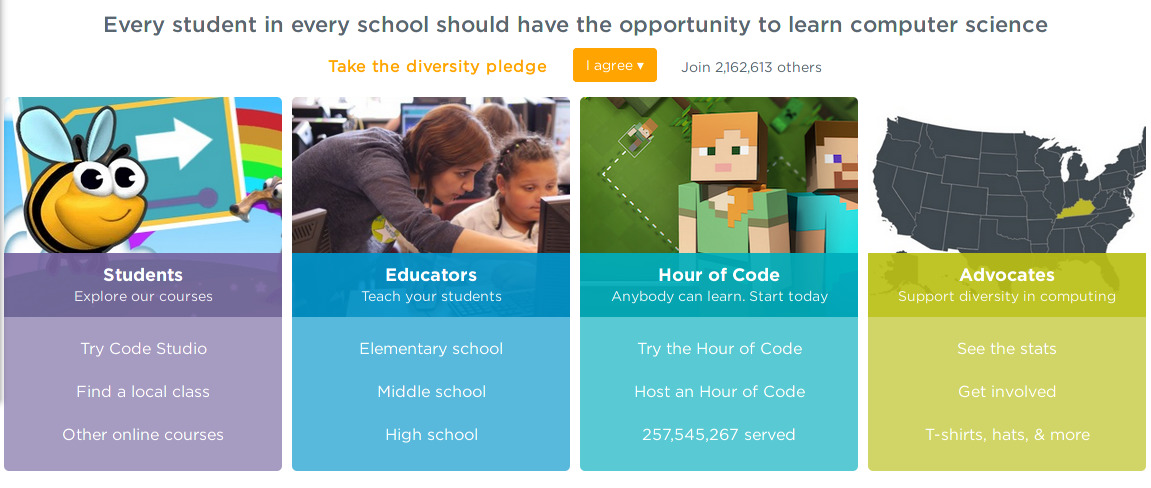
\includegraphics [width=1\linewidth, keepaspectratio =
    1] {./images/sc_web/code_main_part-v01.jpg}
    \caption{Zaslonska slika dela začetne spletne strani
      \emph{\href{https://www.code.org}{code.org}}
      \cite{web:code.org}, iz katerega je razvidna razdeljenost
      vsebin.}
    \label{fig:scr:web:code:main}
\end{figure}

\subsubsection{Ura kode (\emph{ang. Hour of code})}
\label{sec:ura-kode-ang}

\textbf{Ura kode} so krajši projekti, ki jih lahko organizacije, kot so
šole, izvedejo v času ene do dveh ur. Celoten projekt je namenjen
promociji računalniške znanosti in programiranju. Vsebine, ki so v
okviru tega projekta, so navadno uvodne vsebine.

Povezava na portalu \textbf{Ura kode}
\emph{\href{https://code.org}{code.org}} nas vodi do zbirke vadnic, ki
so del spletnega portala \textbf{code}, prav tako najdemo povezave do
številnih drugih spletnih portalov in vsebin, ki so vključene v
projekt, nekatere bomo opisali tudi v nadaljevanju. Vadnice, ki so
del portala, ponujajo številne začetne vsebine, ki so grajene na neki
znani temi iz sveta računalniških iger ali animiranih filmov.

Primer vadnice, ki smo si jo izbrali, je tematsko povzeta iz znane video
igre \textbf{Minecraft}. V uvodu vsake vadnice najprej sledi video
uvod znane osebe, v tem primeru je to glavni razvijalec omenjene
igre. V tem uvodnem delu izvemo, zakaj je postal programer, kaj
bomo počeli v tej uri ter kaj se bomo naučili. V predstavitvi je
predstavljen tudi uporabniški vmesnik vadnice. Uvodni del predstavitve
lahko gledamo kot video ali izberemo zapisan povzetek
predstavitve. Snov, ki je razložena v vadnici, je \textbf{uporaba
  ukazov, zank in vejitev}. Vadnica je sestavljena iz več enot. Med
uvedbo nove snovi spet sledi video predstavitev ali različica v
besedilu.

Vadnice so sestavljene z aplikacijo za programiranje \textbf{Code
  studio} (slika \ref{fig:scr:web:codestudio}). Pisanje programske
kode v njej je omogočeno z \textbf{zlaganjem gradnikov} ali načinom
\emph{ang. Blockly}, kjer z metodo \textbf{vleci in spusti}
sestavljamo oz. zlepljamo programsko kodo. Podoben programski jezik je
tudi \textbf{Scratch}, ki smo ga opisali v poglavju
\ref{sec:scratch}.

\begin{figure}[h!]
  \centering
    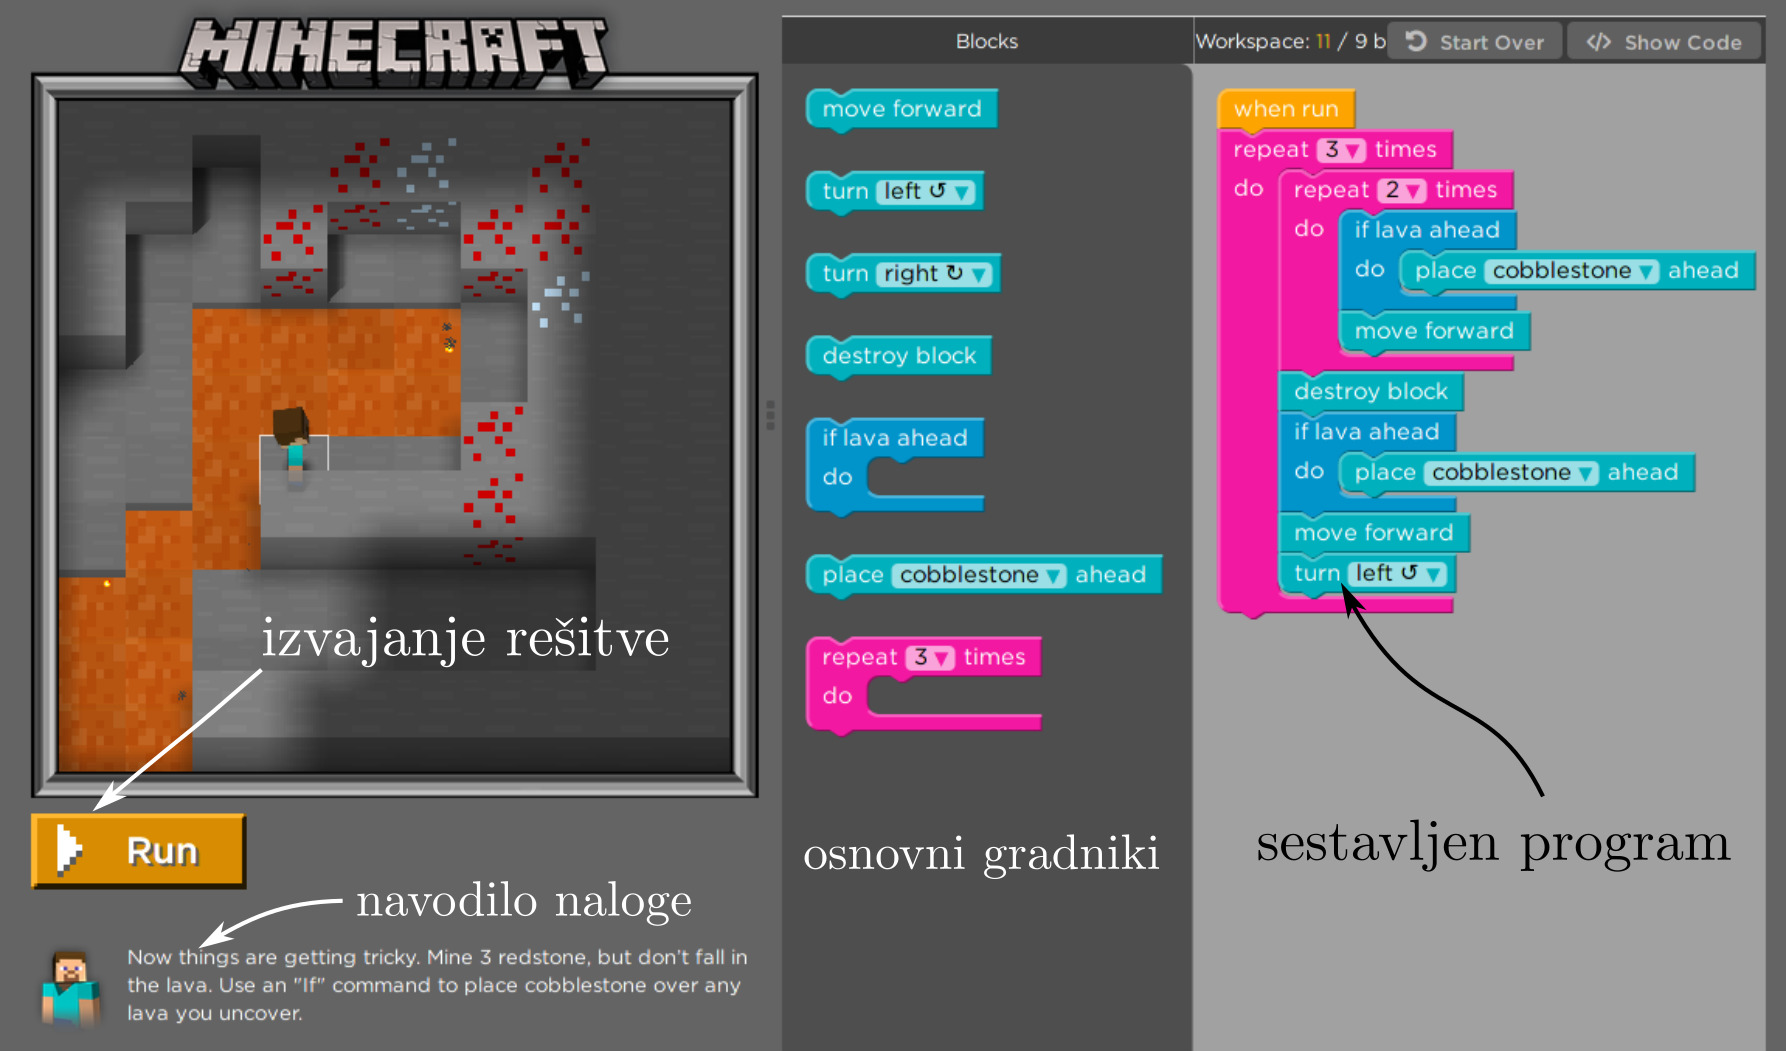
\includegraphics [width=0.65\linewidth, keepaspectratio =
    1] {./images/sc_web/code_cstudiov01.jpg}
    \caption{Spletna aplikacija Code studio, v kateri so zgrajene
      vadnice \cite{web:code.org}.}
    \label{fig:scr:web:codestudio}
\end{figure}

Pod temi zlepljenimi gradniki se ustvarja programska koda v jeziku
\textbf{JavaScript}. Posamezne enote gradijo na znanju sistematično in
postopoma z večanjem težavnostne stopnje. V vadnicah so omogočeni samo
tisti gradniki, ki jih potrebujemo za rešitev naloge. Večina vsebinskih
sklopov je narejena tako, da lahko v zadnji vadnici vsebinskega sklopa 
prosto uporabljamo vse gradniki, ki smo se jih naučili uporabljati ter
nam ni več potrebno izpolniti konkretnega cilja naloge, da jo
opravimo.

\subsubsection{Code studio}
\label{sec:code-studio}

\textbf{Code studio} ni samo spletna aplikacija, ki omogoča vadnice in
pisanje programske kode, temveč je podstran, na kateri novinci najdejo
zbrane vsebinske sklope (slika \ref{fig:scr:web:codestudio:main}), ki so
razdeljeni po težavnosti, ki se ji spreminja spodnja meja starosti,
zgornja ostaja ista pri 18 letih. Posebna značilnost spletne strani je
tudi ta, da ponuja računalniške vsebine, pri katerih ne potrebujemo
računalnika, tako imenovano \textbf{računalništvo brez računalnika}
ali \textbf{izključene vsebine} (\emph{ang. Unplugged lessons}). Te
vsebine so navadno predstavljene s predstavitvenimi videi in gradivi,
ki jih lahko natisnemo. 

\begin{figure}[h!]
  \centering
  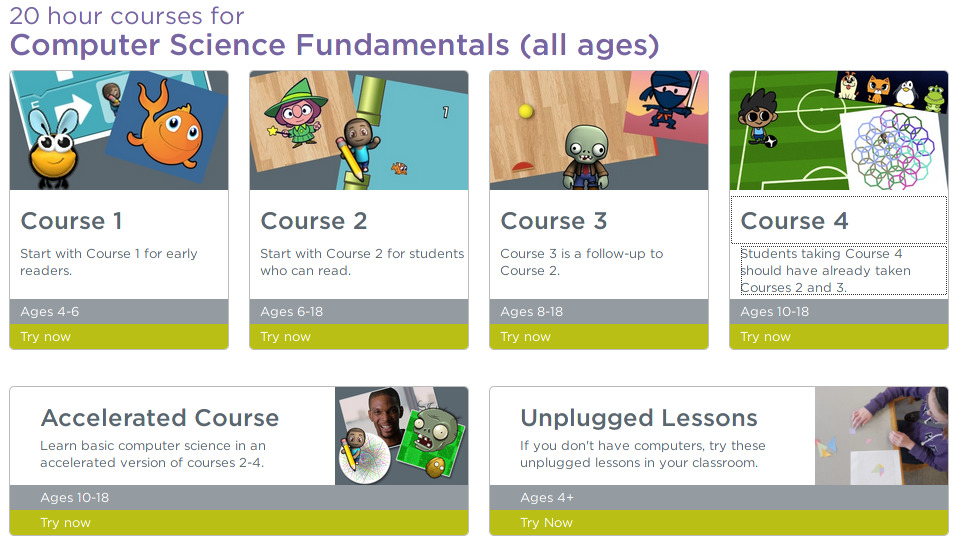
\includegraphics [width=0.65\linewidth, keepaspectratio =
  1] {./images/sc_web/code_cs_main_v01.jpg}
  \caption{Podstran Code studio, kjer lahko nadaljujemo na
    različnih vsebinskih sklopih \cite{web:code.org:studio}.}
  \label{fig:scr:web:codestudio:main}
\end{figure}

S klikom na posamezni vsebinski sklop preidemo na stran s
povzetkom. Na tej strani sledimo tudi lastnemu napredku. Vsebine so
razdeljene na manjše tematske sklope, ki so spet sestavljeni iz
posameznih enot oz. vadnic (slika
\ref{fig:scr:web:codestudio:course}). Med posameznimi tematskimi
sklopi najdemo tudi \textbf{izključene vaje}, ki jih predelujemo brez
računalnika.

\begin{figure}[h!]
  \centering
  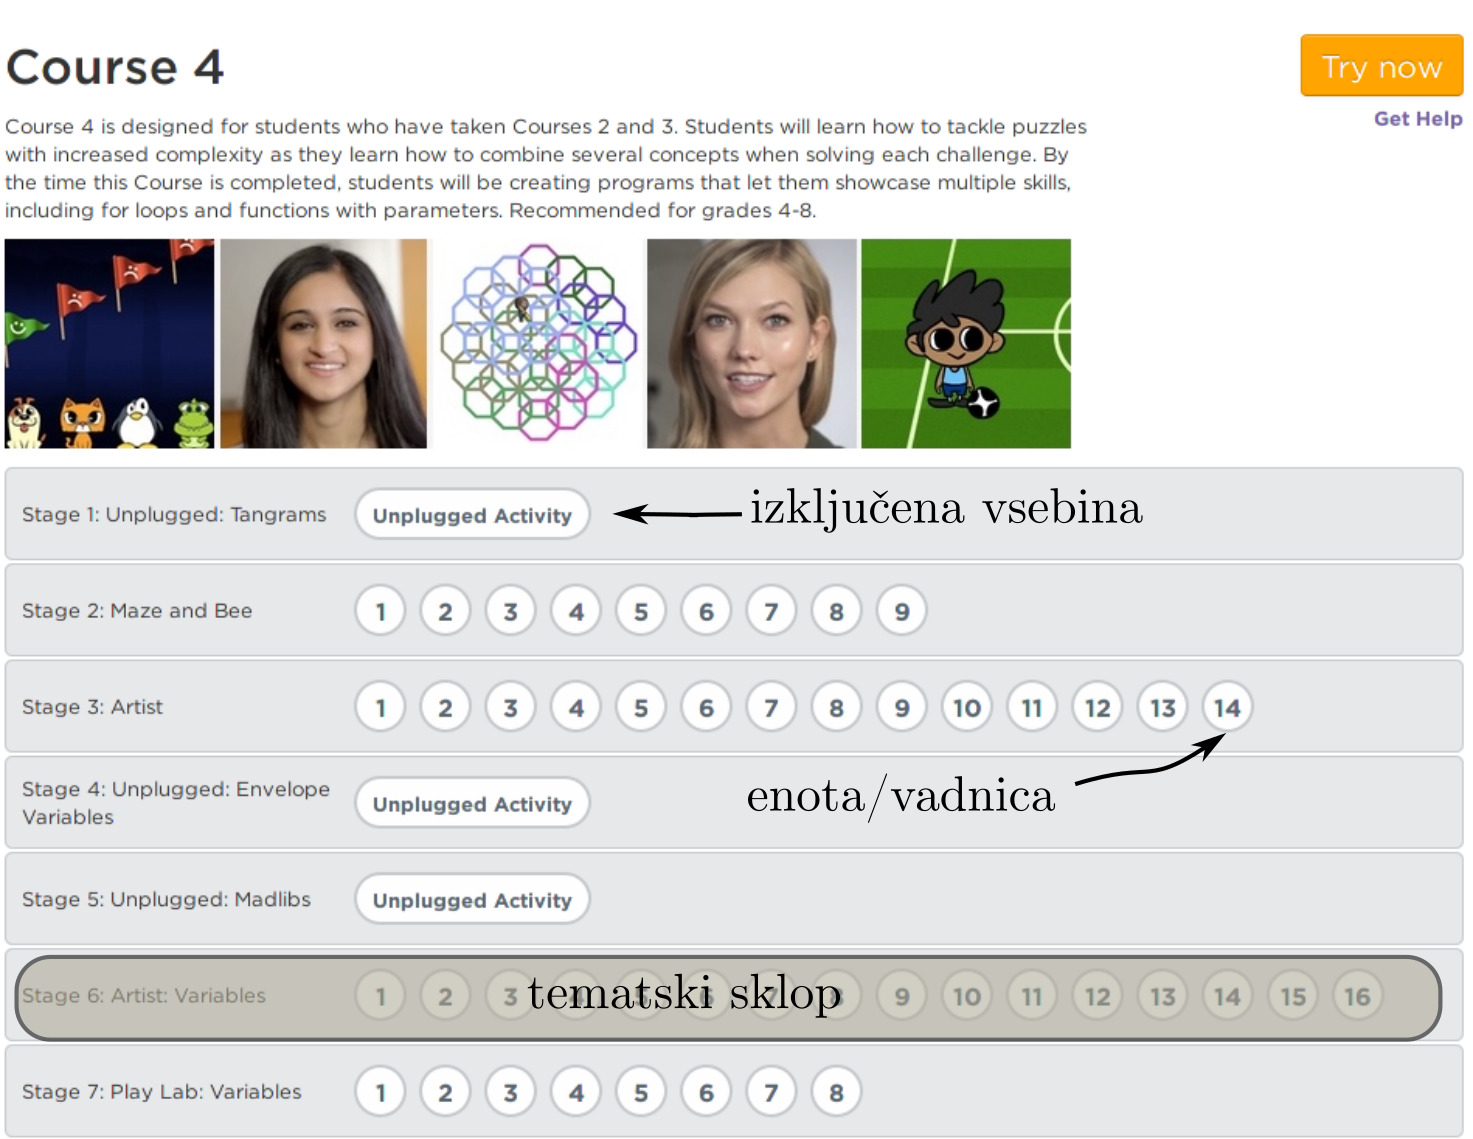
\includegraphics [width=0.65\linewidth, keepaspectratio =
  1] {./images/sc_web/code_course.jpg}
  \caption{Podstran vsebinskega sklopa \cite{web:code.org:studio}.}
  \label{fig:scr:web:codestudio:course}
\end{figure}
  
Reševanje naloge oz. pisanje programa poteka na podoben način, kot smo
ga že predstavili pri enotah \textbf{Ure kode}, vendar je teh enot več
in na vsaki naslednji enoti ponujajo več gradnikov.

\subsubsection{Samostojni projekti}
\label{sec:gradnja-projektov}

Čeprav nekoliko skrito na dnu podstrani \textbf{Code studio}, najdemo
gumb, na katerem piše \emph{\textbf{Moji projekti} (ang. My
  projects}). S pritiskom na gumb preidemo na stran, na kateri lahko
ustvarimo nove projekte, samodejno shranjene projekte ponovno odpremo
ali jih izbrišemo. Ustvarimo lahko naslednje nove projekte,
\textbf{nariši, ustvari igro in ustvari aplikacije}. Ti projekti so
novi in niso omejeni z nobeno vsebino, zato imajo na voljo vse
gradnike.

\textbf{Nariši} (slika \ref{fig:code:mp:draw}) deluje na podobnem
principu kot programski jezik \textbf{Logo}. Imamo pisalo, ki pušča
sled, mi mu s programsko kodo določamo potek, barvo itd. Lahko
ustvarjamo lastne funkcije in uporabljamo že obstoječe, ki jih lahko
spreminjamo. Takšna je npr. \texttt{funkcija nariši hišo}, ki
sprejme argument \texttt{velikost}. Vsi gradniki, ki jih lahko
uporabimo, so omejeni izključno na uporabo pisala. 

Podobno kot nariši uporabljamo \textbf{ustvari igro} (slika
\ref{fig:code:mp:game}). Vendar tu ne uporabljamo pisala, temveč lahko
gradimo igre in zgodbe. Na delu, kjer teče aplikacija, lahko vstavljamo
številne prednastavljene figure, ki se odzivajo na dogodke. Sklopi
ukazov pri obeh oblikah projektov, risanje in igre, so naslednji:
\textbf{akcija, dogodki, zanke, matematika, logika, funkcije in
  spremenljivke}. Kljub številnim možnostim programske logike so
omejitve še vedno prisotne, kot je na primer izbira figur, ki je
omejena, saj lastnih figur ne moremo vstavljati. Uporaba teh dveh
možnosti je namenjena predvsem osnovni šoli.

\begin{figure}[h!]
  \centering
  \begin{subfigure}[]{0.45\textwidth}
    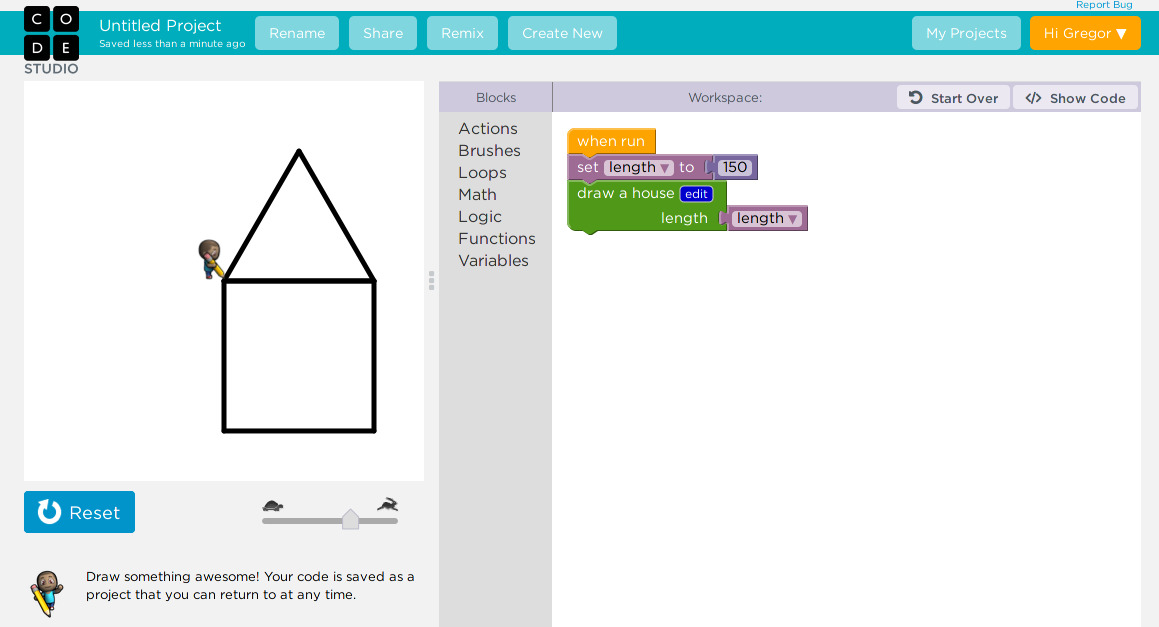
\includegraphics[width=\textwidth]{./images/sc_web/code_cs_draw.jpg}
    \caption{Aplikacija za risanje.}
  \label{fig:code:mp:draw}
\end{subfigure}
\qquad
\begin{subfigure}[]{0.45\textwidth}
  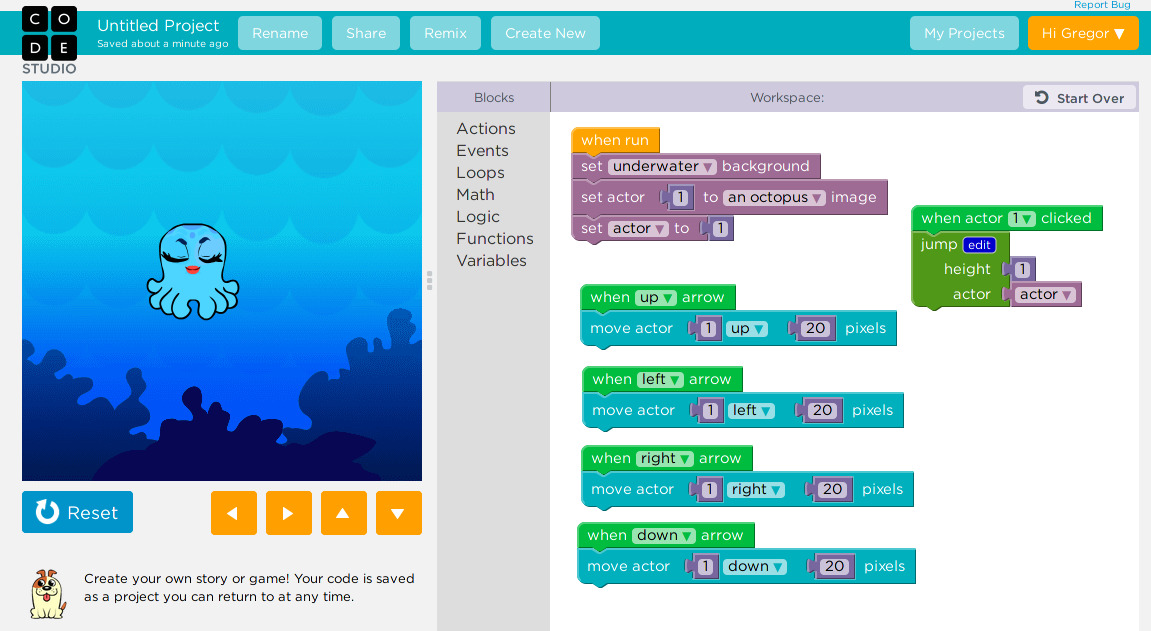
\includegraphics[width=\textwidth]{./images/sc_web/code_cs_game.jpg}
  \caption{Aplikacija za ustvarjanje iger.}
\label{fig:code:mp:game}
\end{subfigure}
\caption{Samostojni aplikaciji za programiranje, primerni za
  osnovno šolo \cite{web:code.org:studio}.}
\label{fig:web:code:mp:dg}
\end{figure}

Naprednejše možnosti za programiranje smo našli v primeru
\textbf{ustvarjanja aplikacij} (slika
\ref{fig:scr:web:code:mp:app}). V tej spletni aplikaciji za
programiranje se lahko odločamo, ali programsko kodo sestavljamo z
gradniki ali jo pišemo tekstovno. Glavna značilnost je ta, da moramo poleg
pisanja programske kode ustvariti še \textbf{uporabniški
  vmesnik}, ki je omejene velikosti. Sestavljanje uporabniškega
vmesnika je podobno sestavljanju mobilni aplikaciji. S programskim
jezikom nismo več tako omejeni in lahko uporabljamo vse vgrajene
funkcije JavaScripta. Vgrajena je tudi dodatna možnost ukaznega izpisa
in osnovni pripomočki za razhroščevanje, \textbf{prekini, preskoči,
  vstopi in izstopi}.

\begin{figure}[h!]
  \centering
    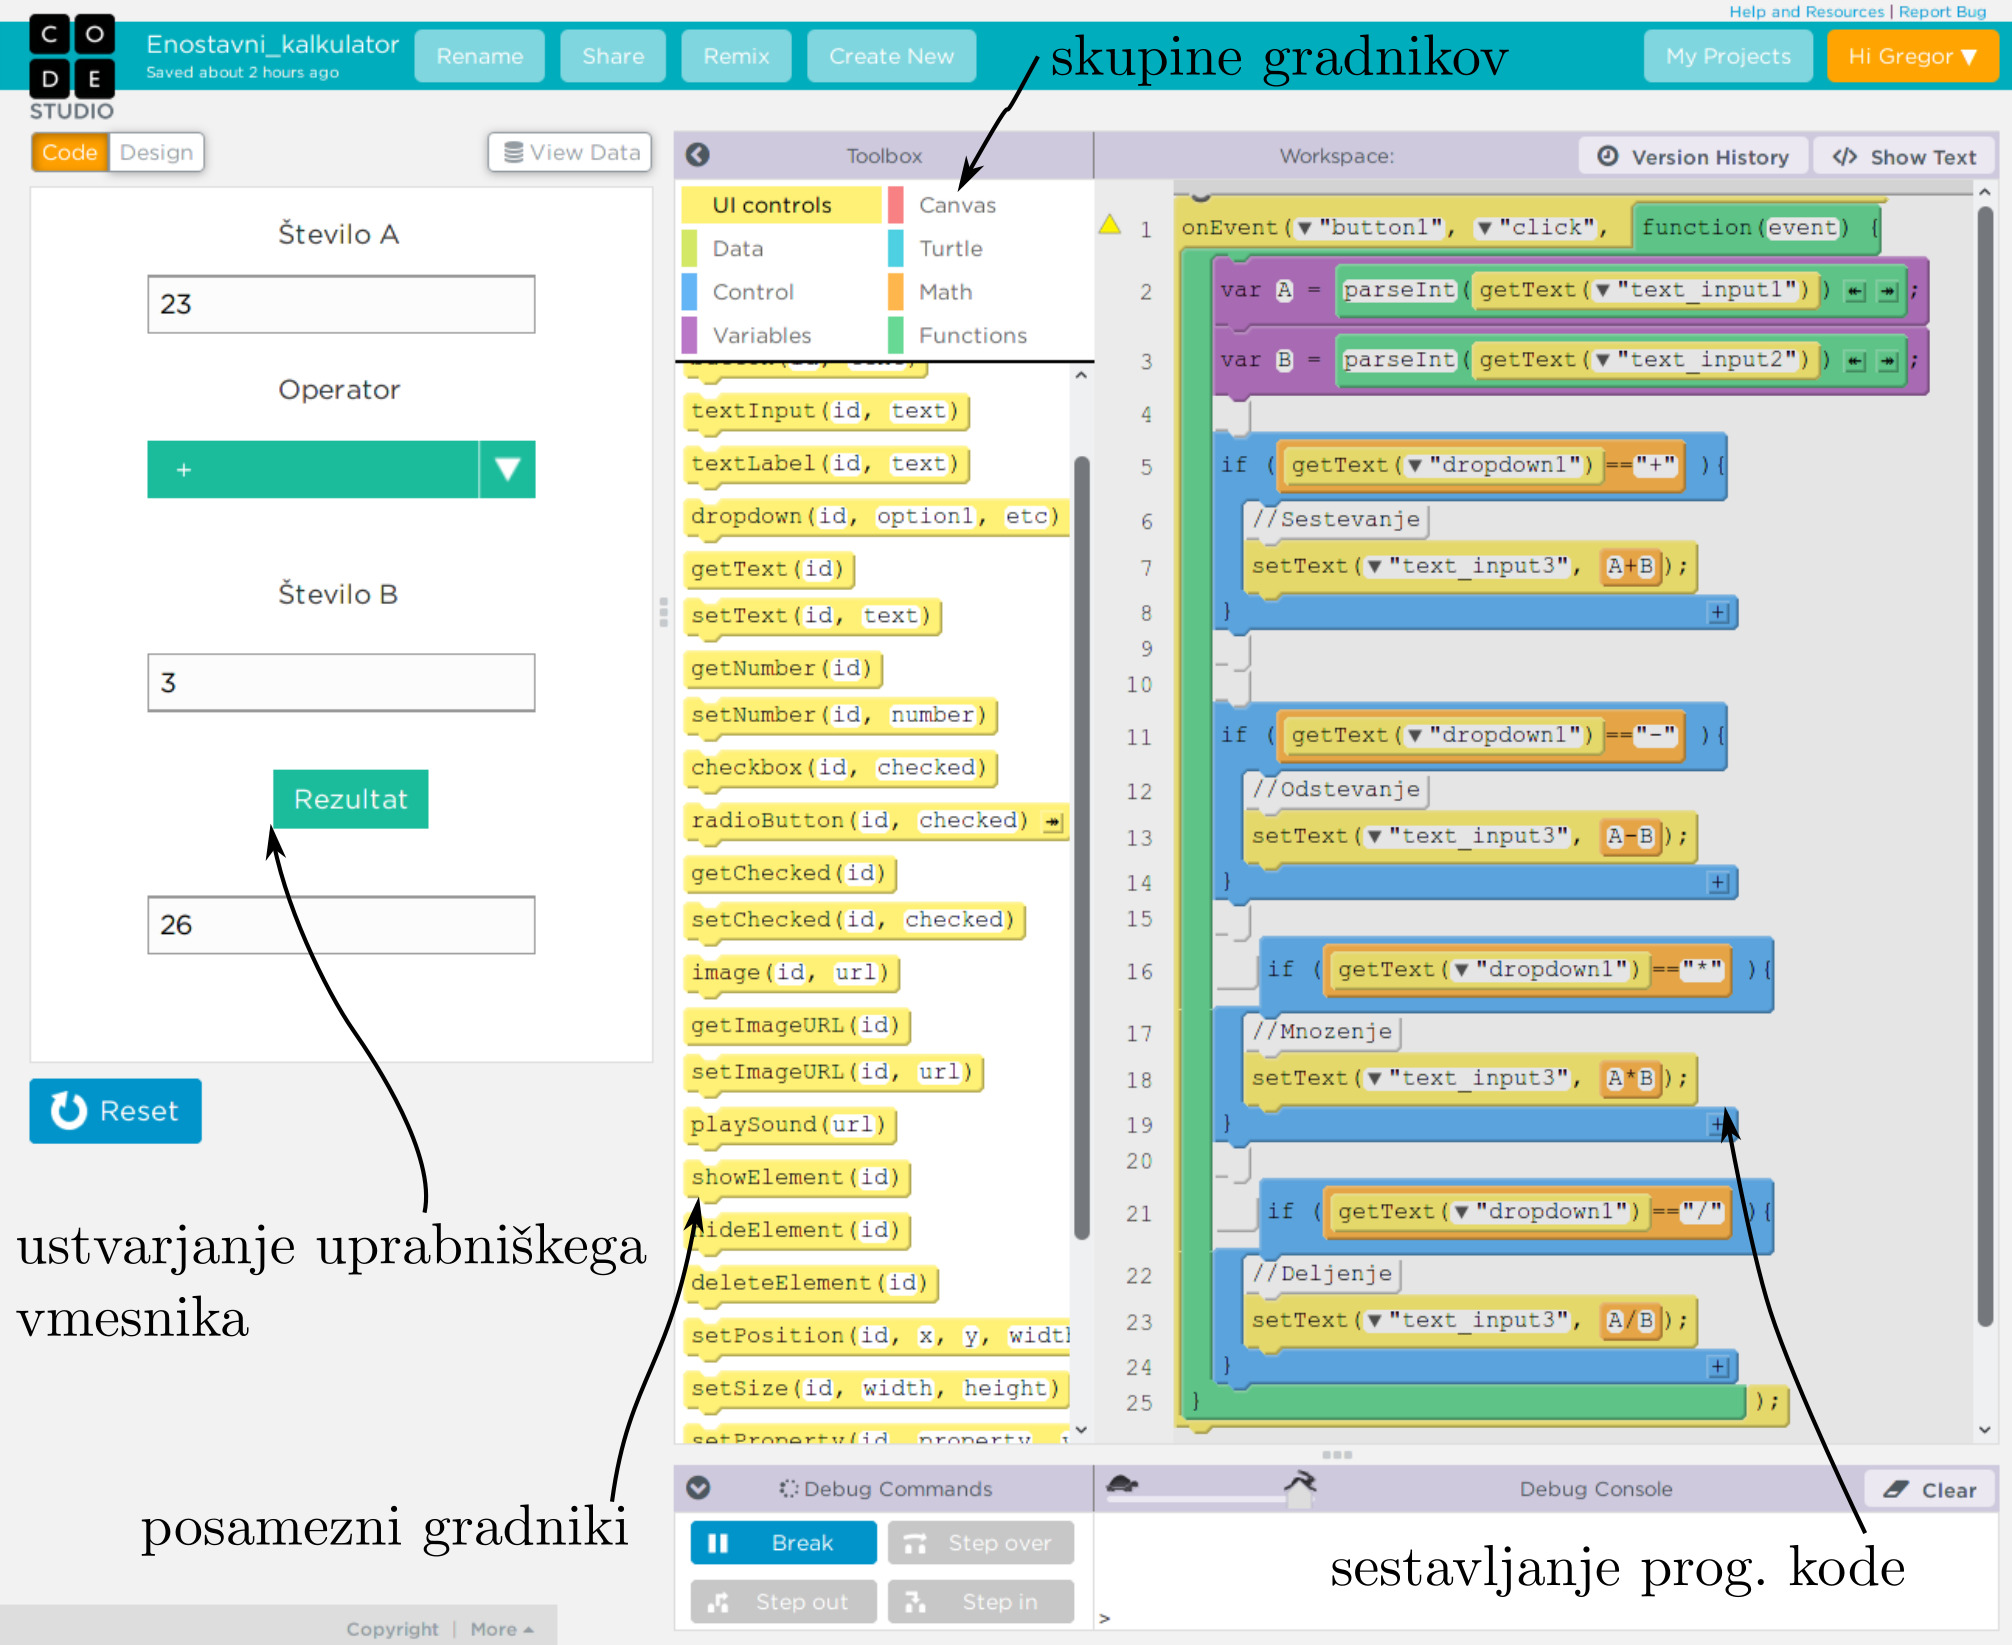
\includegraphics [width=0.90\linewidth, keepaspectratio =
    1] {./images/sc_web/code_cs_mobile.jpg}
    \caption{Spletna aplikacija za programiranje - ustvarjanje
      aplikacij. Primer: preprosto računalo \cite{web:code.org:studio}.}
    \label{fig:scr:web:code:mp:app}
  \end{figure}

\subsubsection{Uporaba za učitelje}
\label{sec:uporaba-za-uitelje}

Celotna vsebina spletnega portala je zasnovana na ameriškem učnem
načrtu. Učitelji na strani najdejo podrobne učne načrte s cilji in
idejami za njihovo realizacijo. 

\subsubsection{Povzetek}
\label{sec:povzetek-code}

Spletni portal velja za glavnega pobudnika \textbf{Ure kode} in
s tem popularizacije učenja računalniške znanosti in programiranja. Na
portalu najdemo ogromno pripravljenih in razdelanih vsebin. Primerna
je predvsem za čiste začetnike \textbf{OŠ} in jo lahko uporabljamo pri
najmlajših učencih. Za \textbf{SŠ} so pripravljene vsebine morda
prelahke in nekoliko otročje, zato jih v ta namen ne bi priporočali,
čeprav zgornje omejitve vadnic ni. Vsebinski sklopi so dobro razdelani
na podrobne enote in ti postopoma stopnjujejo težavnost. Postopnost je
včasih celo pretirana in bi kakšna naloga lahko zajela dve enoti, saj
so posamezni koraki nezahtevni oz. prelahki. Problemska zasnova je
taka, da naloge, ki jih je treba rešiti, izvajajo in rešujejo junaki iz
filmskega oz. sveta video iger. To je pomembno predvsem za motivacijo
najmlajših. Nekatere vadnice so prevedene v slovenski jezik, vendar je
delež prevedenih zanemarljiv. V splošnem lahko rečemo, da večina
spletnega portala ni prevedena. Jezik uporabe spletnega portala pri
pouku ne bi smel ovirati, saj so naloge razdelane na majhne dele in so
navodila preprosta, tako jih lahko učitelj podaja sproti ustno ali jih
ima pripravljene na učnih listih po posameznih korakih. Celotna
razporeditev na spletnem portalu včasih deluje nestrukturirana in
neurejena. 

Kot samostojne aplikacije v primeru \textbf{risanja in ustvarjanja
  iger} so uporabne, vendar so po zmožnostih dokaj omejene, zato lahko
v ta namen z večjo svobodo in izbiro uporabljamo
Scratch. \textbf{Ustvarjanje aplikacij} je primerno predvsem za
srednje šole, omogoča pisanje programske kode, prav tako lahko
posamezne dele kode nazorno predstavimo grafično z gradniki. Uporabna
je predvsem v uvodu gradnje aplikacij, saj ustvarjamo uporabniški
vmesnik in programsko kodo sami od začetka.

\begin{osebnabox}[label={osebna:code.org}]{Code | \url{code.org}}
    \begin{tabular}{
  p{0.30\linewidth-2\tabcolsep} |
  p{0.70\linewidth-2\tabcolsep}  }
  \textbf{Vrsta vsebine} & Napredna kombinirana vsebina: vadnica
                           (video vodič + navodila (naloga) + spletna
                           aplikacija za programiranje). \\
      \hline 
  \textbf{Jezik spletne strani} &  Angleščina: da, slovenščina: da
                                  (nekatere vadnice),
                                  drugi: ne. \\
      \hline
  \textbf{Ponujena znanja} & Osnove rač. znanosti in programiranja. \\
      \hline
  \textbf{Programski jeziki} & Blocky (podobno kot Scratch),
                               JavaScript. \\
      \hline
  \textbf{Težavnostna stopnja} & Osnovna šola (vadnice, risanje,
                                 ustvarjanje iger), srednja šola
                                 (ustvarjanje aplikacij). \\
      \hline
  \textbf{Upoštevanje načel} & Upošteva načelo sistematičnosti: da,
      postopnosti: da, problemski pristop: da. \\
      \hline
  \textbf{Dosežki/Gamification} & Ne. \\
      \hline
  \textbf{Dodajanje lastnih vsebin} & Ne. \\
      \hline
  \textbf{Upravljanje razreda} & Ne. \\
      \hline
  \textbf{Dostop vsebin} & Brezplačno. \\
\end{tabular}
\end{osebnabox}
\subsection{Codeacademy}

Spletni portal je tipični predstavnik novonastalih portalov za učenje
programiranja. Sami o sebi pravijo, da so ameriško podjetje, ki se
ukvarja z izobraževanjem. Njihov tim se ukvarja z ustvarjanjem spletne strani
\emph{\href{https://www.codecademy.com/}{Codeacademy}} ter se uči in
poučuje, saj želijo ustvariti najboljšo spletno izobraževalno izkušnjo
za prihodnost, ki domuje na spletu \cite{web:codeacademy}. Po
registraciji in prijavi nas čaka naslednja spletna stran (slika
\ref{fig:scr:web:codeacademy}). Z začetne, nadzorne strani lahko
izbiramo nov vsebinski sklop ali nadaljujemo z že začetimi.

\begin{figure}[h!]
  \centering
    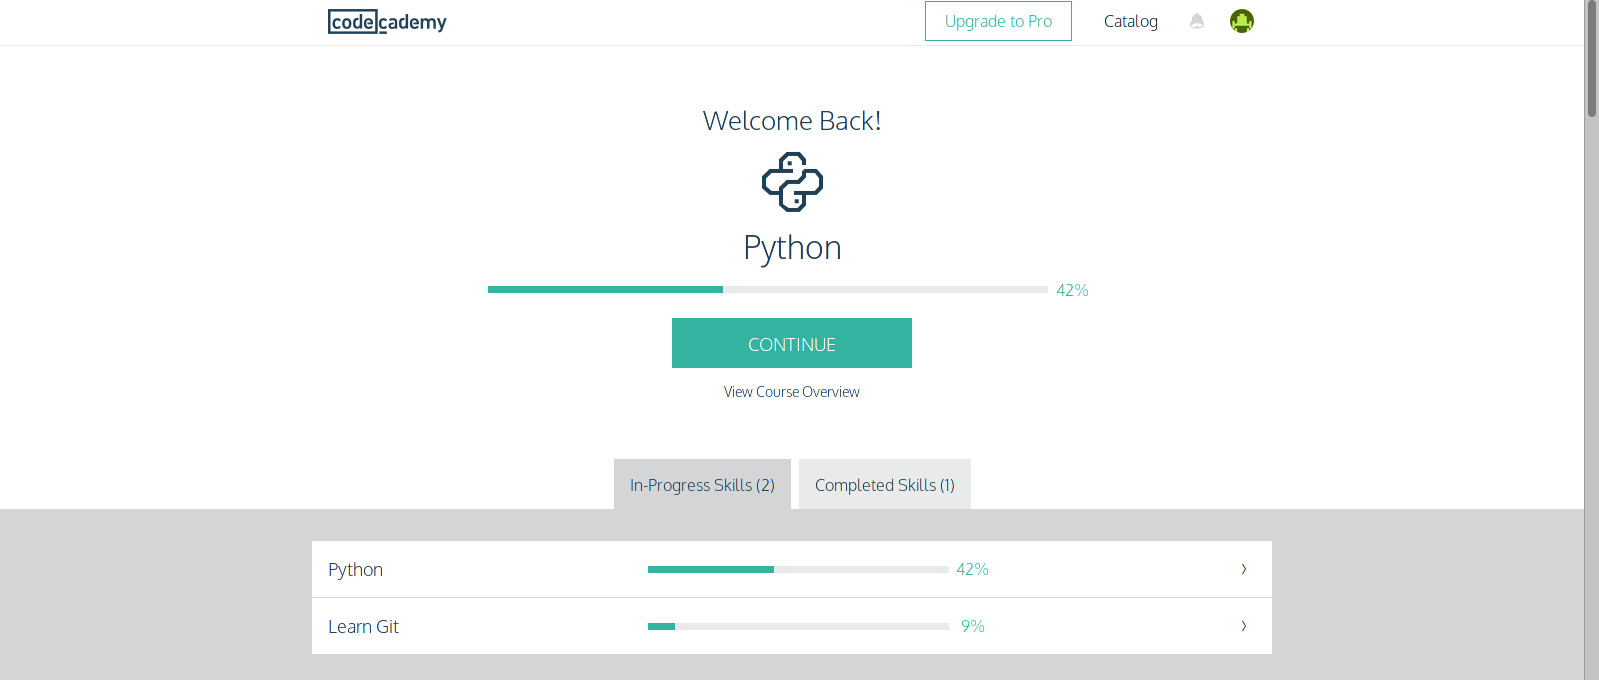
\includegraphics [width=0.65\linewidth, keepaspectratio =
    1] {./images/sc_web/codeacademy_login_01.jpg}
    \caption{Zaslonska slika spletne strani
      \emph{\href{https://www.codecademy.com/}{Codeacademy}}
      \cite{web:codeacademy}. Začetna, nadzorna stran po prijavi, od
      tu nadaljujemo na vsebinske sklope, ki smo jih že začeli.}
    \label{fig:scr:web:codeacademy}
\end{figure}

\textbf{Jezik} spletne strani je v \textbf{angleščini}, drugih jezikov ni
mogoče izbrati. Če še podrsamo po spletni strani navzdol, najdemo
vsebinske sklope, ki učijo programske jezike in so naslednji: \textbf{HTML+
  CSS, JavaScript, JQuery, PHP, Python, Ruby} in že v prejšnjem odseku
so bile na voljo osnove \textbf{Jave}.

\begin{figure}[h!]
  \centering
    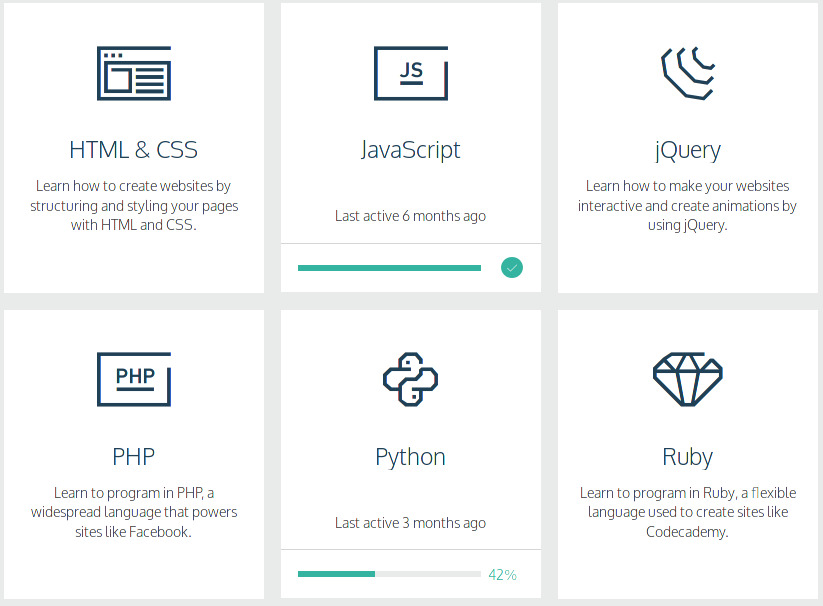
\includegraphics [width=0.65\linewidth, keepaspectratio =
    1] {./images/sc_web/codeacademy_vescine_02.jpg}
    \caption{Zaslonska slika spletne strani
      \emph{\href{https://www.codecademy.com/}{Codeacademy}}
      \cite{web:codeacademy}. Seznam znanj/veščin programskih jezikov,
      ki jih ponuja spletni portal.}
    \label{fig:scr:web:codeacademy:vescine-prog}
\end{figure}

Nad zbirko osnovnih programskih jezikov najdemo druga
\textbf{ponujena znanja}. V tem delu najdemo nekatere vsebine, kot je
na primer, učenje \textbf{SQL}, uporaba \textbf{ukazne vrstice} ali
uporaba spletnega orodja za nadzor različice \textbf{GIT}. Nekatere
vsebine so sestavljene kot projekti, taki sta na primer \textbf{naredi
  spletno stran} ali \textbf{naredi spletno stran interaktivno}. 
Strnemo lahko, da spletni portal ne ponujajo le znanja in veščine
\textbf{programiranja in programskih jezikov}, temveč tudi druga
znanja. S klikom na želeno vsebino pridemo na stran (slika
\ref{fig:scr:web:codeacademy:tema}), s katere lahko nadaljujemo tam,
kjer smo ostali ali pregledujemo posamezne teme, ki smo jih že
opravili ali tiste, ki nas še čakajo.


% \begin{figure}[h!]
%   \centering
%     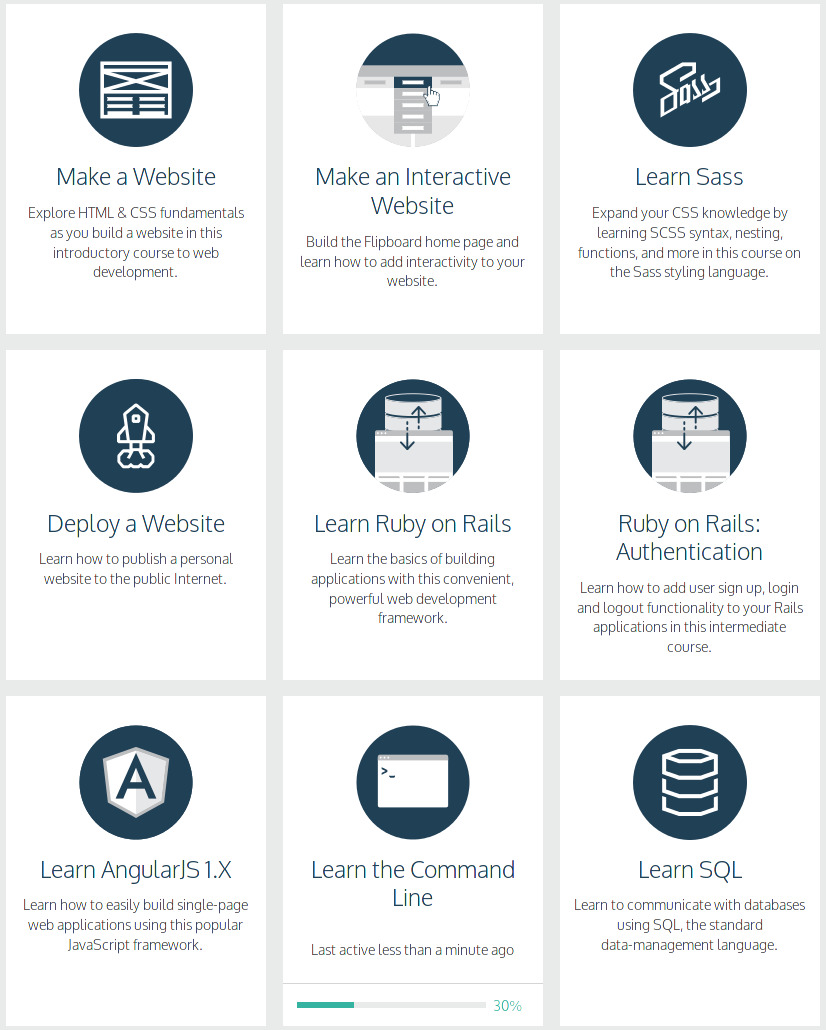
\includegraphics [width=0.65\linewidth, keepaspectratio =
%     1] {./images/sc_web/codeacademy_vescine_01.jpg}
%     \caption{Zaslonska slika spletne strani
%       \emph{\href{https://www.codecademy.com/}{Codeacademy}}
%       \cite{web:codeacademy}. Seznam znanj/veščin, ki jih ponuja
%       spletni portal.}
%     \label{fig:scr:web:codeacademy:vescine-web}
% \end{figure}

\begin{figure}[h!]
  \centering
    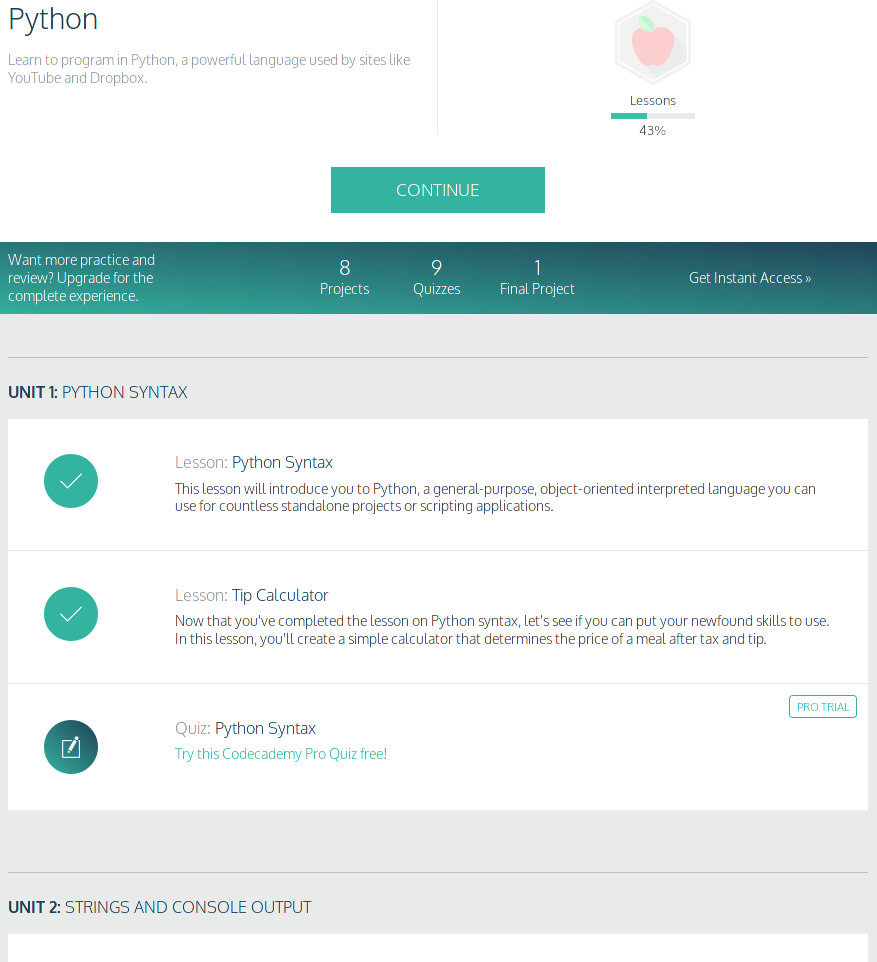
\includegraphics [width=0.65\linewidth, keepaspectratio =
    1] {./images/sc_web/codeacademy_tema_01.jpg}
%  \def\svgwidth{\columnwidth}
%  \input{./pdf_tex/codeacademy_tema_01.pdf_tex}
  \caption{Zaslonska slika podstrani spletne strani
      \emph{\href{https://www.codecademy.com/}{Codeacademy}}
      \cite{web:codeacademy}, na kateri lahko pregledujemo posamezne
      teme in nadaljujemo tam, kjer smo ostali.}
    \label{fig:scr:web:codeacademy:tema}
\end{figure}

Razvidno je, da so teme sistematično razporejene, zato lahko ugotovimo,
da je \textbf{načelo sistematičnosti upoštevano}. S pritiskom na gumb
za nadavaljevanje (\emph{ang. Continue}) odpremo urejevalnik (slika
\ref{fig:scr:web:codeacademy:ide}) na temi in podenoti, na kateri smo
ostali.

\begin{figure}[h!]
  \centering
    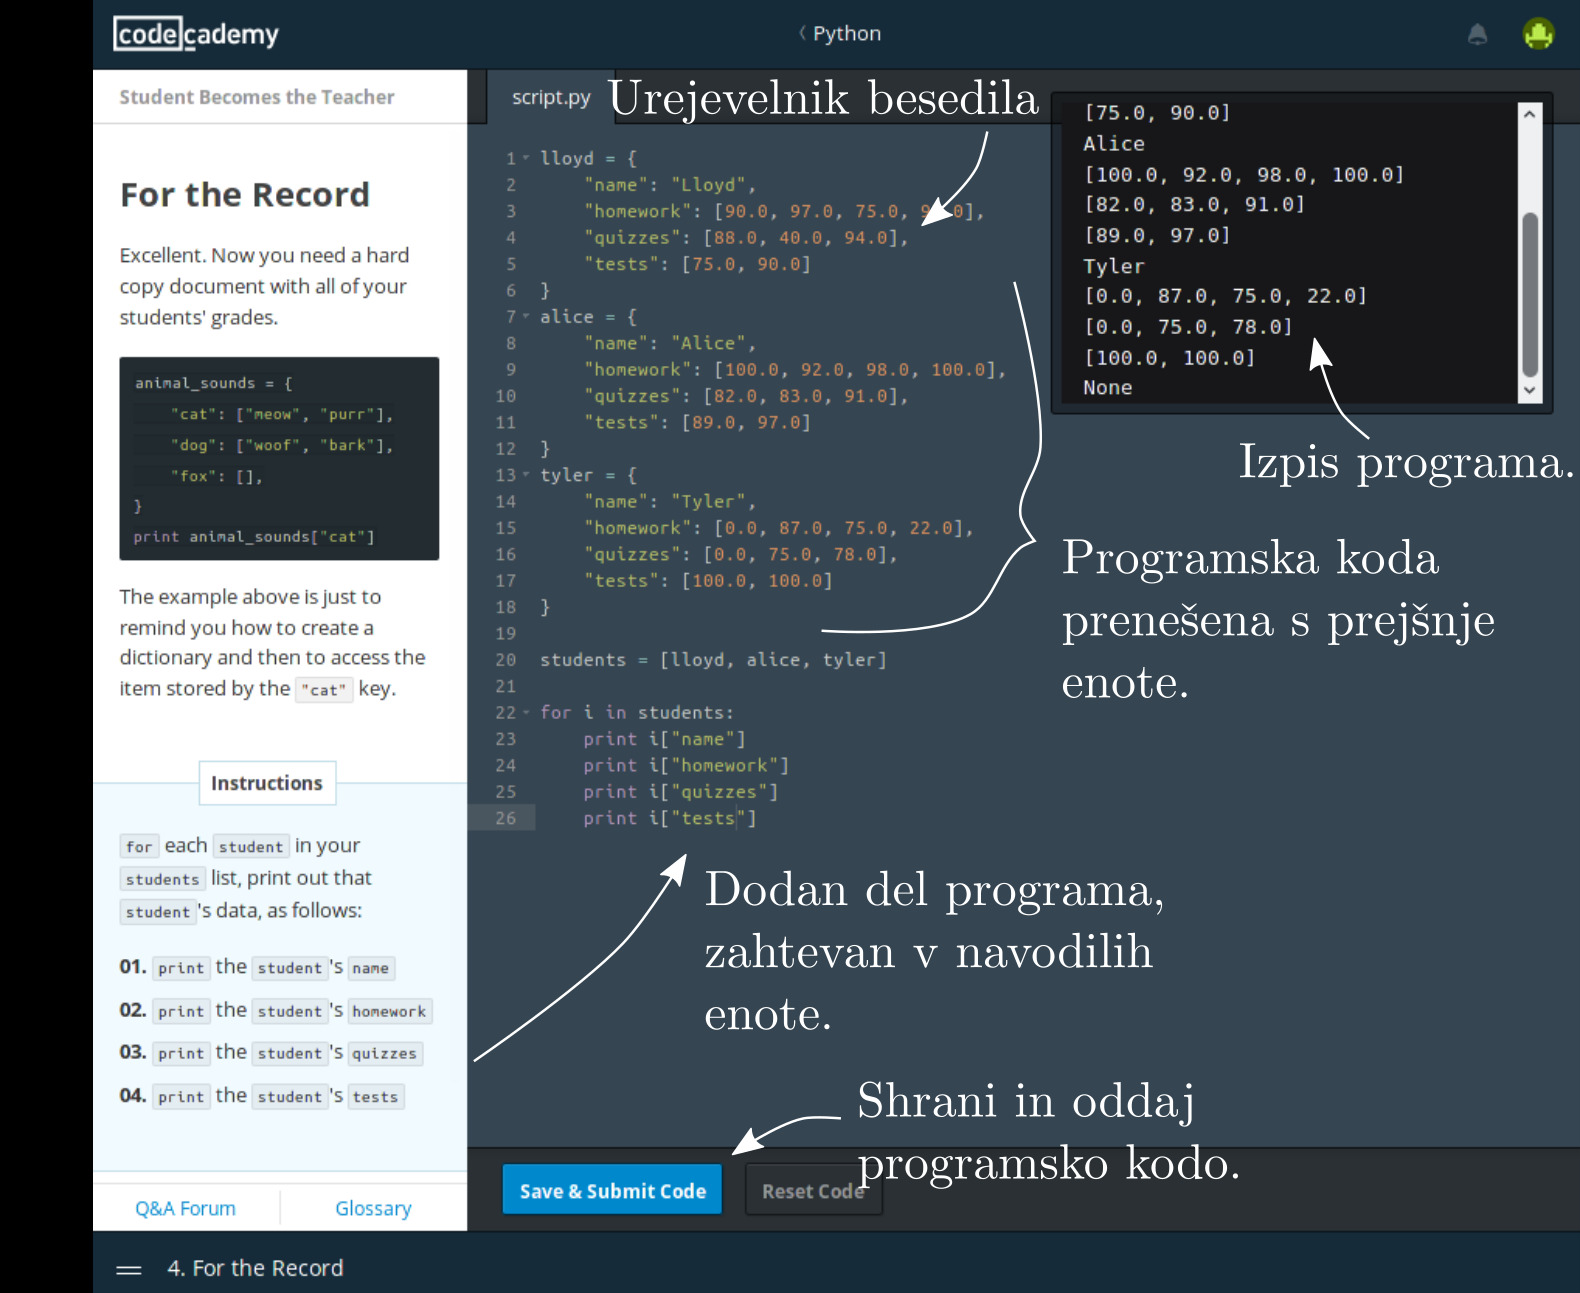
\includegraphics [width=0.65\linewidth, keepaspectratio =
   1] {./images/sc_web/codeacademy_IDE_02.jpg}
   \caption{Zaslonska slika
     \emph{\href{https://www.codecademy.com/}{Codeacademy}}
     \cite{web:codeacademy} vadnice, ki jo sestavlja urejevalnik z
     navodili in oknom za izpis v programu.}
    \label{fig:scr:web:codeacademy:ide}
\end{figure}

Vsaka tema vsebinskega sklopa je razdeljena na več enot oz. vadnic, ki
so sestavljene tako, da postopoma dograjujejo program. Delo, ki smo ga
opravili v predhodni vadnici, se samodejno prenese naprej, ko je to
potrebno. Lahko povemo, da je \textbf{načelo postopnosti
  upoštevano}. Pri nekaterih tematskih sklopih sledi najprej ponovitev
že naučenega. Na primer pri temi \emph{seznami in funkcije} najprej
sledi pregled osnovnega upravljanja s seznami in pisanjem funkcij.
Uporabniški vmesnik (slika \ref{fig:scr:web:codeacademy:ide}) je
urejen tako, da imamo na desni strani podano snov, ki je sestavljena s
\textbf{primerom določene programske strukture in navodili}, kaj
moramo dograditi v programu. Na levi strani imamo \textbf{urejevalnik
  besedil}, v katerega pišemo programsko kodo. Urejevalnik zna barvati
programsko kodo in samodejno predviditi zamike besedila. V zgornjem
desnem kotu je \textbf{okno za izpis}, v katerem se izpisujejo
\textbf{izhodni podatki} iz programa in napake sintakse \textbf{Python
  tolmača}. Spodaj je gumb za \textbf{shrani in oddaj programsko kode}
(\emph{ang. Save and Submit Code}).

Vsaka v uvodnem delu predstavi novo problematiko, ki jo potem v
posameznih enotah rešujemo. Vsebina je predstavljena
\textbf{problemsko}. Samo delo z \textbf{vadnico} poteka tako, da
napišemo program v \textbf{spletno aplikacijo za programiranje}, ki je
zahtevan v navodilih. Ko menimo, da imamo pravilno rešitev, pritisnemo
na gumb \textbf{shrani in oddaj programsko kodo.} Program najprej
preverja \textbf{sintaktično} pravilnost. Napako program vrne nad
gumbom za oddajo programske kode, podrobna napaka \textbf{Pythonovega
  tolmača} se izpiše v \textbf{oknu za izpis}. Zatem sledi
\textbf{semantično} preverjanje pravilnosti rešitve naloge. V
posamezni enoti program samodejno vrši osnovno preverjanje programa s
točno določenim rezultatom. Dokler test napisanega programa ne da
pravega rezultata, ne moremo nadaljevati na naslednjo enoto. Ko se nam
zatakne, spletna stran ponuja \textbf{forum}, na katerem najdemo
odgovor ali lahko postavimo vprašanje. Forum je razdeljen na posamezne
teme in enote, tako da lahko hitro najdemo zahtevano vprašanje.

%Zbiranje dosežkov
Za uspešno premagovanje enot je uporabnik nagrajen z
\textbf{značkami}, ki so vidne na strani njegovega profila. Na tej
strani se beležijo tudi predelane vsebine. Spletni portal torej
uporablja nagrajevanje z \textbf{dosežki}.

Spletni portal ponuja tudi plačljive vsebine, čeprav je osnova
vsebinskih sklopov brezplačna. Za dostop do plačljivih storitev 
ponujajo model zakupa z naročnino za  \textbf{19\$/mesec}. Za
naročnino uporabnik pridobi dostop do\textbf{ naslednjih dodatnih
  storitev}:

\begin{itemize}
\item personaliziran učni načrt,
\item dostop do kvizov,
\item dostop do realnih projektov,
\item dostop pomoči v živo preko sporočil.
\end{itemize}

Ugotovimo, da je spletni portal \textbf{polplačljivi} in da dodatne
storitve, ki jih ponuja spletni portal, niso potrebne za uporabo pri
pouku, saj vse omenjene dodatne storitve lahko zagotovi učitelj.

\subsubsection{Uporaba za učitelje}
\label{sec:uporaba_učitelji}

Spletni portal nudi vsebine, ki so prilagojene za šole in uporabo v
šolah. V pregledu lahko ugotovimo, da za srednješolske profesorje
ponujajo naslednje:

\begin{itemize}
\item \textbf{trening za učitelje}, ki je možen le v ZDA,
\item \textbf{gradiva},
\item \textbf{sledenje napredku učencem},
\item \textbf{ura kode} (ang. \emph{Hour of code}).
\end{itemize}

Podstran z \textbf{ gradivi} %(slika \ref{fig:scr:web:codeacademy:tr})
profesorju ponuja razdelane posamezne teme na enote, podobno kot so
razdelane na glavni strani. Pod vsako enoto lahko profesor preizkusi,
rešuje vaje. Večina enot ima pripravljene kvize, ki jih profesor lahko
prav tako preizkusi in se pripravi na učno uro.

% \begin{figure}[h!]
%   \centering
%     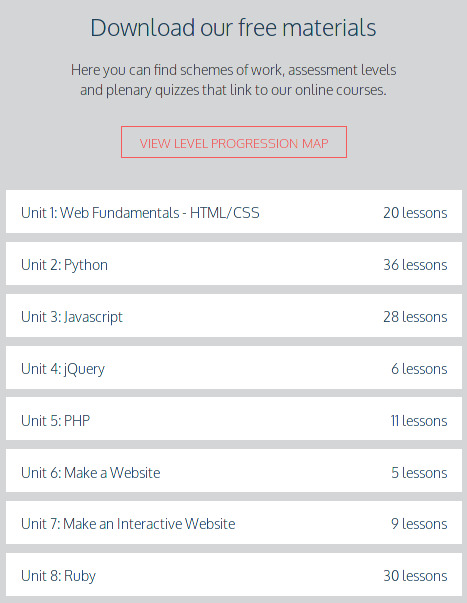
\includegraphics [width=0.40\linewidth, keepaspectratio =
%    1] {./images/sc_web/codeacademy_tr_01.jpg}
%    \caption{Zaslonska slika
%      \emph{\href{https://www.codecademy.com/}{Codeacademy}}
%      \cite{web:codeacademy} pod strani z gradivi in tematskimi
%      sklopi.} %%NI ukazna vrstica temveč ...
%     \label{fig:scr:web:codeacademy:tr}
% \end{figure}

Kot so si zamislili avtorji spletnega portala, so tematski sklopi in
posamezne enote med seboj prepletene in vodijo do posameznega
cilja. Zemljevid (slika \ref{fig:codeacademy:poster}) prikazuje
povezavo enot na posamezni stopnji in različne cilje. Za vsak tematski
sklop lahko učitelj prenese \textbf{pregled posamezne teme}, v kateri
so podrobneje zapisani učni cilji in so označene stopnje, ki sovpadajo
z zemljevidom.

\begin{figure}[h!]
  \centering
    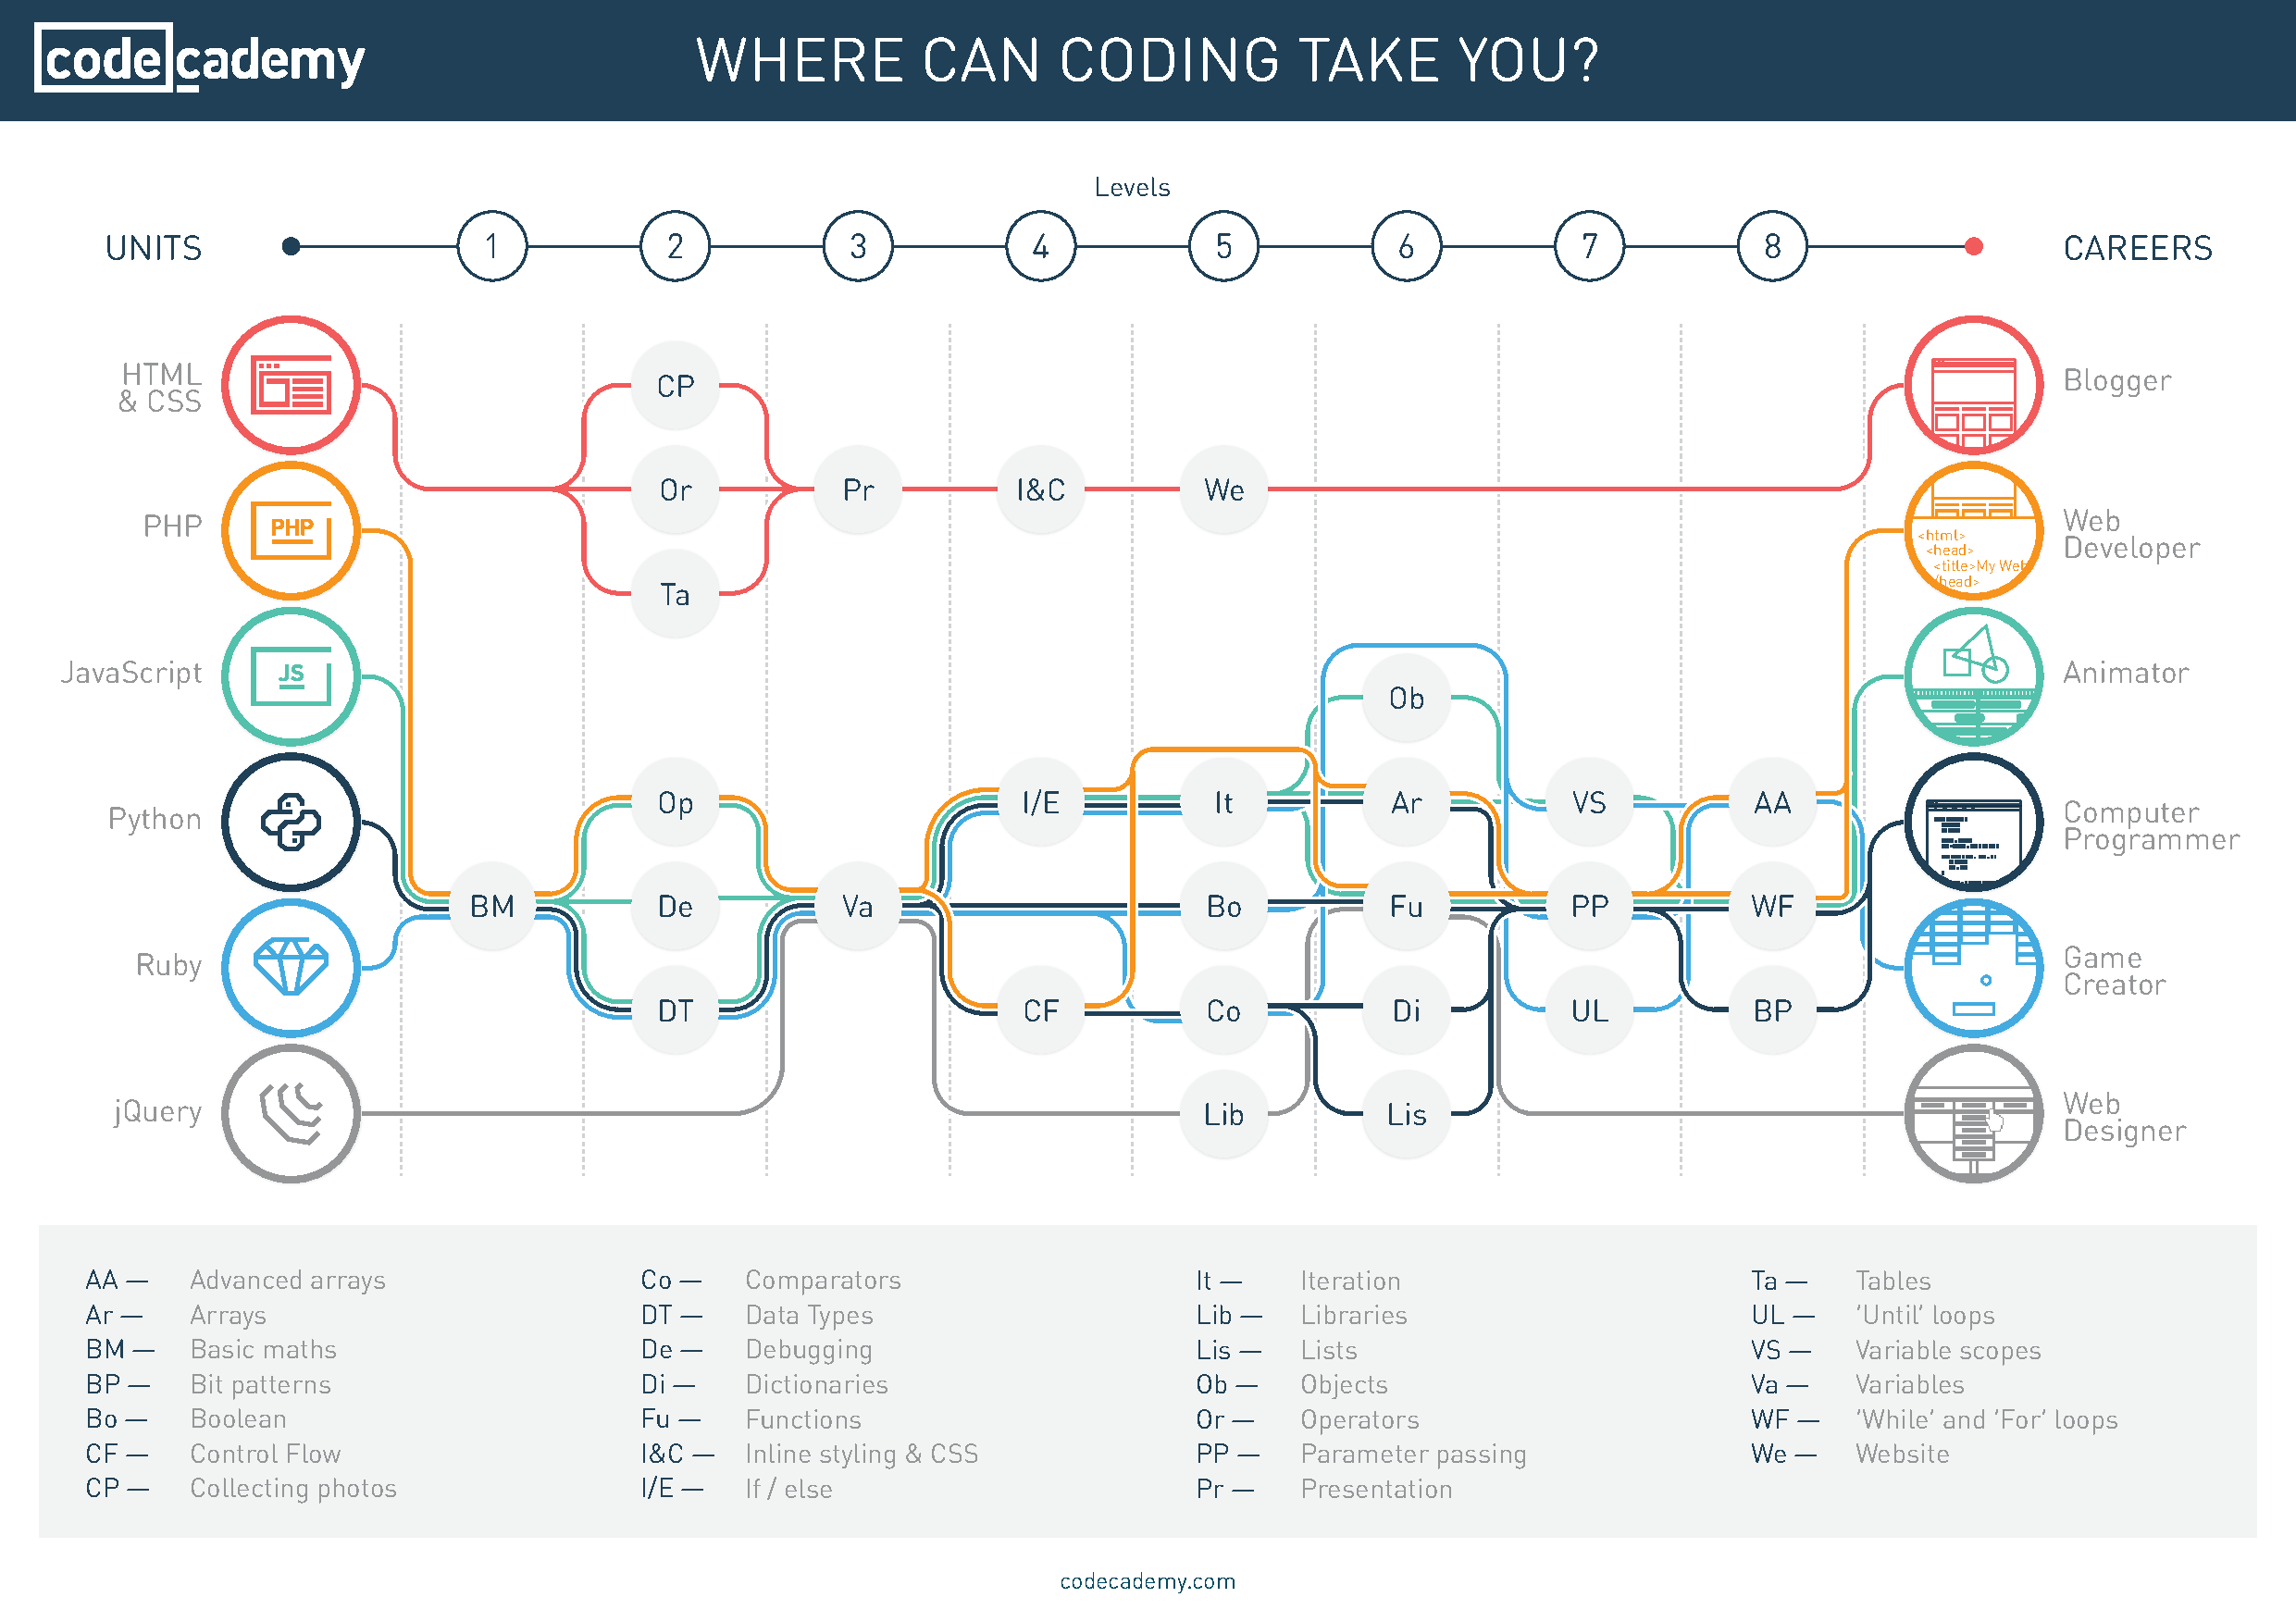
\includegraphics [width=1\linewidth, keepaspectratio =
   1] {./images/CAdemy-poster.pdf}
   \caption{Plakat s povezavami enot različnih tematskih sklopov po
     stopnjah, ki vodijo  do posameznih ciljev (\emph{ang. Level
       prograsion mapa}) \cite{web:codeacademy}.}
    \label{fig:codeacademy:poster}
\end{figure}

Ena izmed naprednih zmožnosti spletnega portala je \textbf{sledenje
  napredku učencem} (\emph{ang. Students tracking}). Ta omogoča, da
profesor dijakom ustvari račune in jih povabi na spletnem portalu v
razred. Določi tematske sklope, katerim bo sledil. V pregledu (slika
\ref{fig:scr:web:codeacademy:tracking}) lahko profesor opazuje
napredek posameznega dijaka po enotah ali v povzetku za celotni
napredek. Napredek je prikazan s pikami različnih barv, ki
predstavljajo odstotke napredka pri posameznem tematskem sklopu. V tem
primeru \textbf{ne moremo} govoriti o \textbf{upravljanju razreda},
saj je omogočeno le sledenje napredku in ne tudi komunikacija med
profesorjem in dijakom, prav tako ni mogoče dodajati lastnih enot
oz. nalog. Pri samem ustvarjanju razreda je profesorju delo zelo
olajšano, saj portal omogoča, da informacije o dijakih ustvarjalec
razreda kopira neposredno s programa, podobnega kot je \textbf{Excel}. V
tabeli so podani podatki \textbf{ime, priimek, skupina, uporabniško
  ime}. Dijaki za dostop do spletnega portala uporabijo uporabniško
ime, ki si ga izmisli učitelj ali oni sami, geslo je skupno za celotno
učilnico. S prejetim uporabniškim imenom in geslom se dijaki na
spletni strani registrirajo s svojim elektronskim naslovom. Če so na portalu
že registrirani, profesorju posredujejo uporabniško ime in jih ta doda
v ustvarjen razred. Dijak mora povabilo potrditi.

\begin{figure}[h!]
  \centering
    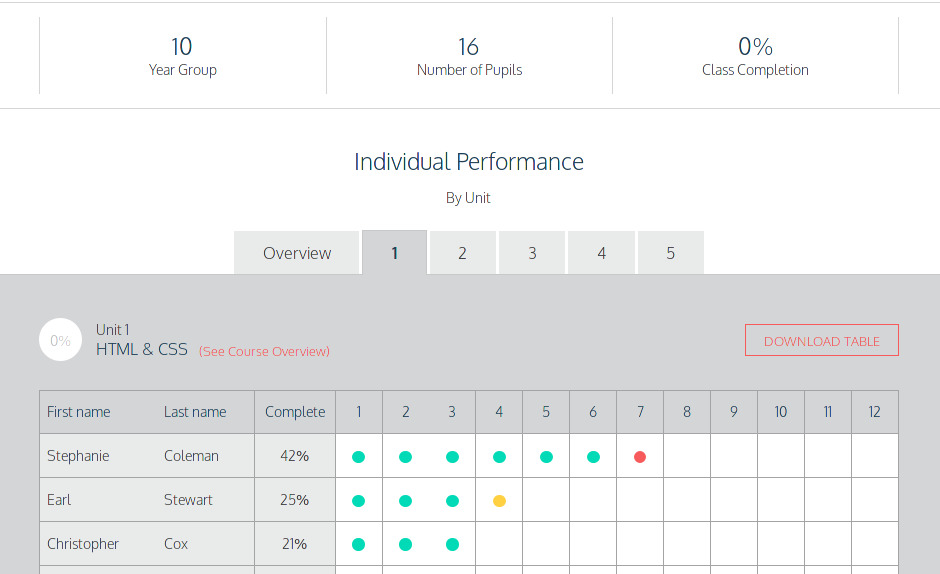
\includegraphics [width=0.65\linewidth, keepaspectratio =
   1] {./images/sc_web/codeacademy_tracking_01.jpg}
   \caption{Zaslonska slika
     \emph{\href{https://www.codecademy.com/}{Codeacademy}}
     \cite{web:codeacademy}. Prikazuje tabelo za sledneje napredku
     učencem.}
    \label{fig:scr:web:codeacademy:tracking}
\end{figure}

\subsubsection{Povzetek}

\emph{\href{https://www.codecademy.com/}{Codeacademy}}
\cite{web:codeacademy} ima dobro razdelano vsebino, ki je na nekaterih
delih dokaj poglobljena. Sistematičnost, postopnost in problemski
pristop so prav tako dobro zastavljeni. Portal ponuja številne
projektne vsebine in učenje programskih jezikov. Izbor teh je tak, da
ustreza današnjim spletnim tehnologijam in zahtevam. Znanje se omejuje
predvsem na učenje programiranja ter da se to znanje zna uporabiti v
praktične namene. Spletni portal ima nekatere vsebine in zmožnosti
plačljive, ampak ima zadostno število brezplačnih vsebin, ki omogočajo
normalno učenje. 

Zanemarjeno je znanje \textbf{računalniške znanosti}, saj se med
spoznavanjem programskih jezikov in podatkovnih struktur ne uči
različnih algoritmov. Uči se bolj uporabo posameznih funkcij, ki so
vgrajene v programski jezik. Slaba stran spletnega portala je ta, da
je v celoti v \emph{angleškem jeziku}. Poleg tujega jezika so nekatera
navodila napisana dokaj kompleksno in zahteva že dobro poznavanje
razumevanja sporočil tolmača in semantičnih napak, ki se zgodijo v
programu.

Spletni portal je v primeru učenja spletnih tehnologij, kot je
\textbf{HTML/CSS}, je primeren za učence zadnje triade osnovne šole,
saj se ti omenjeno snov učijo pri izbirnem predmetu
\textbf{računalniška omrežja}. V primeru učenja programskega jezika
\textbf{Python} spletni portal ponuja zahtevna znanja in je primeren
predvsem za srednje in višje šole.

Da bi mentor lahko spletni portal uporabljal pri pouku, bi moral imeti
prevode navodil za posamezno temo in enoto. Vsekakor ga je možno izvesti
kot \emph{praktično vodeno delo}. Spletni portal se lahko uporablja za
domače delo in smo uporabo kot takega opisali v poglavju
\ref{sec:prim-uresn-cil-ss}. Mentor lahko spletni portal priporoča v
uporabo kot neobvezno dopolnilno dejavnost tistim dijakom, ki
želijo razširiti znanje programiranja. Opozorimo, da jim lahko
priporoča le brezplačne vsebine. Čeprav je možno, pa vseeno morda ni
primerno uporabljati spletni portal tako, da bi z njim predelali
celoten vsebinski sklop in bi ga pri pouku uporabljali kot edino
orodje, saj je poučevanje računalniške znanosti na njem omejeno. Lahko pa
ga s pridom uporabimo kot dodatek pri učenju programskega jezika,
kot je na primer \textbf{Python}, ki v nadaljevanju služi kot orodje
za poučevanje računalniške znanosti. Pri pouku smo omejeni tudi s
spreminjanjem vsebine, ki je ni mogoče prilagoditi učnemu načrtu
tako, kot bi to želeli, zato moramo učno pripravo prilagoditi uporabi
spletnega portala. Poleg prednosti in slabosti lahko zaključimo, da
ima spletni portal še dodatno motivacijsko vrednost, saj njegova
sistematičnost in postopnost ter nagrajevanje z dosežki motivira
uporabnike, da imajo željo po dokončanju vsebinskega sklopa, ki ga
obravnavajo. 

\begin{osebnabox}[label={osebna:codeacademy}]{Codeacademy | \url{www.codeacademy.com}}
    \begin{tabular}{
  p{0.30\linewidth-2\tabcolsep} |
  p{0.70\linewidth-2\tabcolsep}  }
  \textbf{Vrsta vsebine} & Napredna kombinirana vsebina: vadnica
                           (primer +  navodilo (vodič) + spletna
                           aplikacija za programiranje).  \\
      \hline
  \textbf{Jezik spletne strani} &  Angleščina: da, slovenščina: ne,
                                  drugi: ne. \\
      \hline
  \textbf{Ponujena znanja} & Znanje prog. jezikov, druge vsebine. \\
      \hline
 \textbf{Programski jeziki} & \textbf{HTML+ CSS}, Java JavaScript, Jquery, PHP,
                              \textbf{Python}, Ruby. \\
      \hline
  \textbf{Težavnostna stopnja} & 3/3 osnovna šola, srednja šola. \\
      \hline
   \textbf{Upoštevanje načel} & Upoštevanje načela sistematičnosti: da,
      postopnosti: da, problemski pristop: da. \\
      \hline
  \textbf{Dosežki/Gamification} & Da (značke). \\
      \hline
  \textbf{Dodajanje lastnih vsebin} & Ne. \\
      \hline
  \textbf{Upravljanje razreda} &Da, ustvarjanje razreda in sledenje
                                 napredku učencem. \\
      \hline
  \textbf{Dostop vsebin} & Polplačljiv (plačljivi so projekti, kvizi,
                           podpora v živo). \\
\end{tabular}
\end{osebnabox}

\subsection{Scratch}
\label{sec:scratch}

Spletni portal \emph{\href{https://scratch.mit.edu/}{Scratch}}
\cite{web:scratch} je spletna različica zelo popularnega programskega
jezika \textbf{Scratch}. Scratch je pri nas popularen predvsem v
\textbf{osnovnih šolah} in je zamenjal dolgo uporabljen \textbf{Logo}.

Razvoj samostojne namizne različice Scratcha se je končal pri različici
1.4, od tu naprej je razvoj Scratcha potekal za spletno
različico. Spletna različica je narejena na osnovi zaprtega
\textbf{Adobe Flasha}. Za poganjanje Scratcha v spletnem brskalniku
potrebujemo vtičnik \textbf{Flash}. Ko prvič naložimo spletni portal
\emph{\href{https://scratch.mit.edu/}{Scratch}} (slika
\ref{fig:web:scratch:main}), lahko ugotovimo, da ponuja naslednje
funkcionalnosti:

\begin{itemize}
\item ustvarjanje programov (orodje Scratch),
\item deljenje ustvarjenih programov,
\item raziskovanje narejenih programov, drugih uporabnikov,
\item forum za diskusijo,
\item pomoč pri uporabi.
\end{itemize}

\begin{figure}[h!]
  \centering
    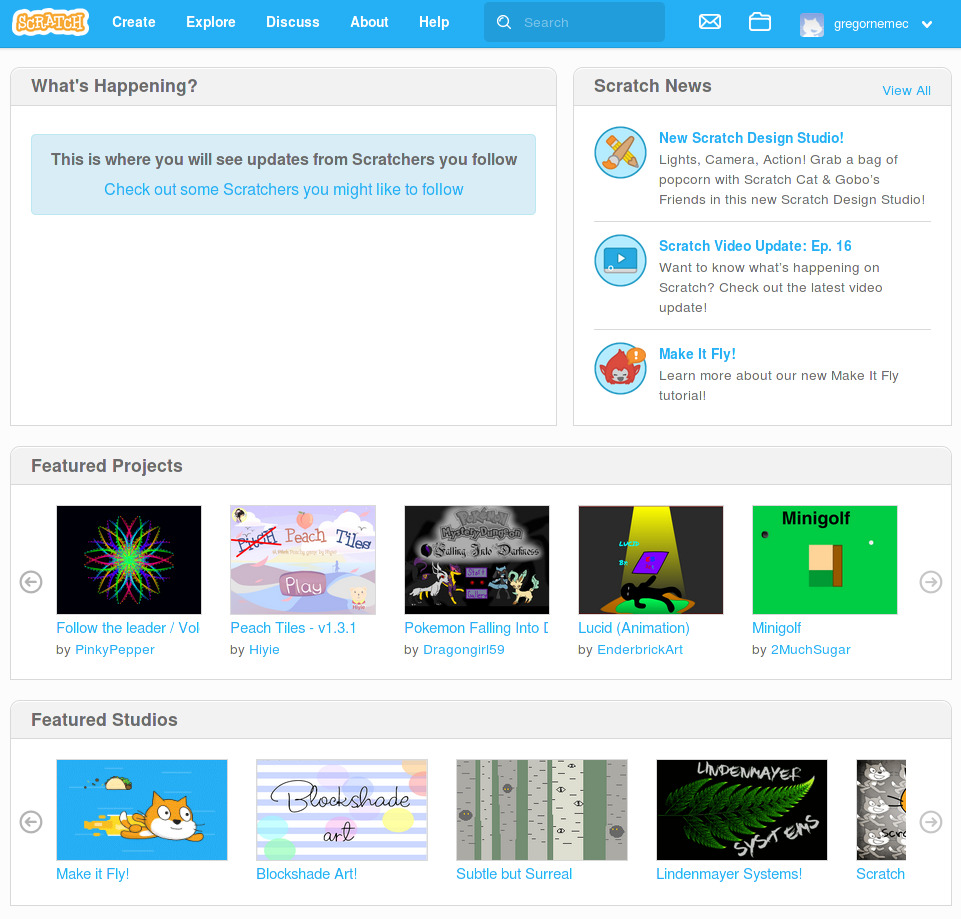
\includegraphics [width=0.65\linewidth, keepaspectratio =
   1] {./images/sc_web/scratch_mainP-v01.jpg}
   \caption{Zaslonski posnetek glavne strani
     \emph{\href{https://scratch.mit.edu/}{Scratch}}
     \cite{web:scratch}.}
    \label{fig:web:scratch:main}
\end{figure}

Scratch smo po vrsti vsebine umestili med \textbf{spletne aplikacije
  za programiranje} oz. smo ga predstavili kot samostojno
\textbf{orodje}. Lastne vsebine, ki bi v širšem smislu poučevala
računalniško znanje, ne najdemo. Vse vsebine, ki so na strani, so
namenjene učenju uporabe orodij in spoznavanju zmožnosti programskega
jezika. Vseeno lahko govorimo o spletnem portalu, saj ima ta vse za
uspešno uporabo orodja in omogoča vso funkcionalnost, ki jo potrebuje
neka spletna skupnost.

\subsubsection{Uporaba Scratcha}
\label{sec:uporaba_scratcha}

Scratch omogoča ustvarjanje animacij, predstavitev in iger. Namenjen je učencem, starim od
8 do 16 let, vendar ne predstavlja nobene omejitve na zgornji
meji starosti. Preveden je v številne jezike, med njimi je tudi
\textbf{slovenščina} \cite{web:scratch:about}.

Če smo v preteklosti že uporabljali namizno različico Scratcha, nam
uporaba spletne različice (slika \ref{fig:web:scratch:orodje}) ne bo
predstavljala nobenih težav, saj je postavitev uporabniškega vmesnika
zelo podobna, kot je bilo to v namizni različici. Osnovni princip
delovanja je tak, da na \emph{oder} (slika
\ref{fig:web:scratch:orodje}) postavljamo različne \emph{like}. Vsak
lik, ki ga dodamo iz knjižnice ali ga naložimo sami, je predstavljen
kot svoj objekt in vsakemu posebej dodajamo programsko kodo, ki jo
sestavljamo iz različnih \emph{gradnikov}. V samem orodju lahko
dorisujemo k že obstoječim likom, rišemo nove ali jih naložimo
neposredno iz računalnika. Dodajamo lahko tudi zvok, ki ga posnamemo
sami ali ga izberemo iz knjižnice zvokov. Programsko kodo lepimo
skupaj oz. sestavljamo podobno, kot bi sestavljali kocke. Kot smo že
spoznali, takemu načinu sestavljanja programske kode pravimo tudi
\emph{``Blocky''}. Gradniki so oblikovani tako, da se sklopijo samo
tisti, ki se med sabo lahko povežejo.

\begin{figure}[h!]
  \centering
    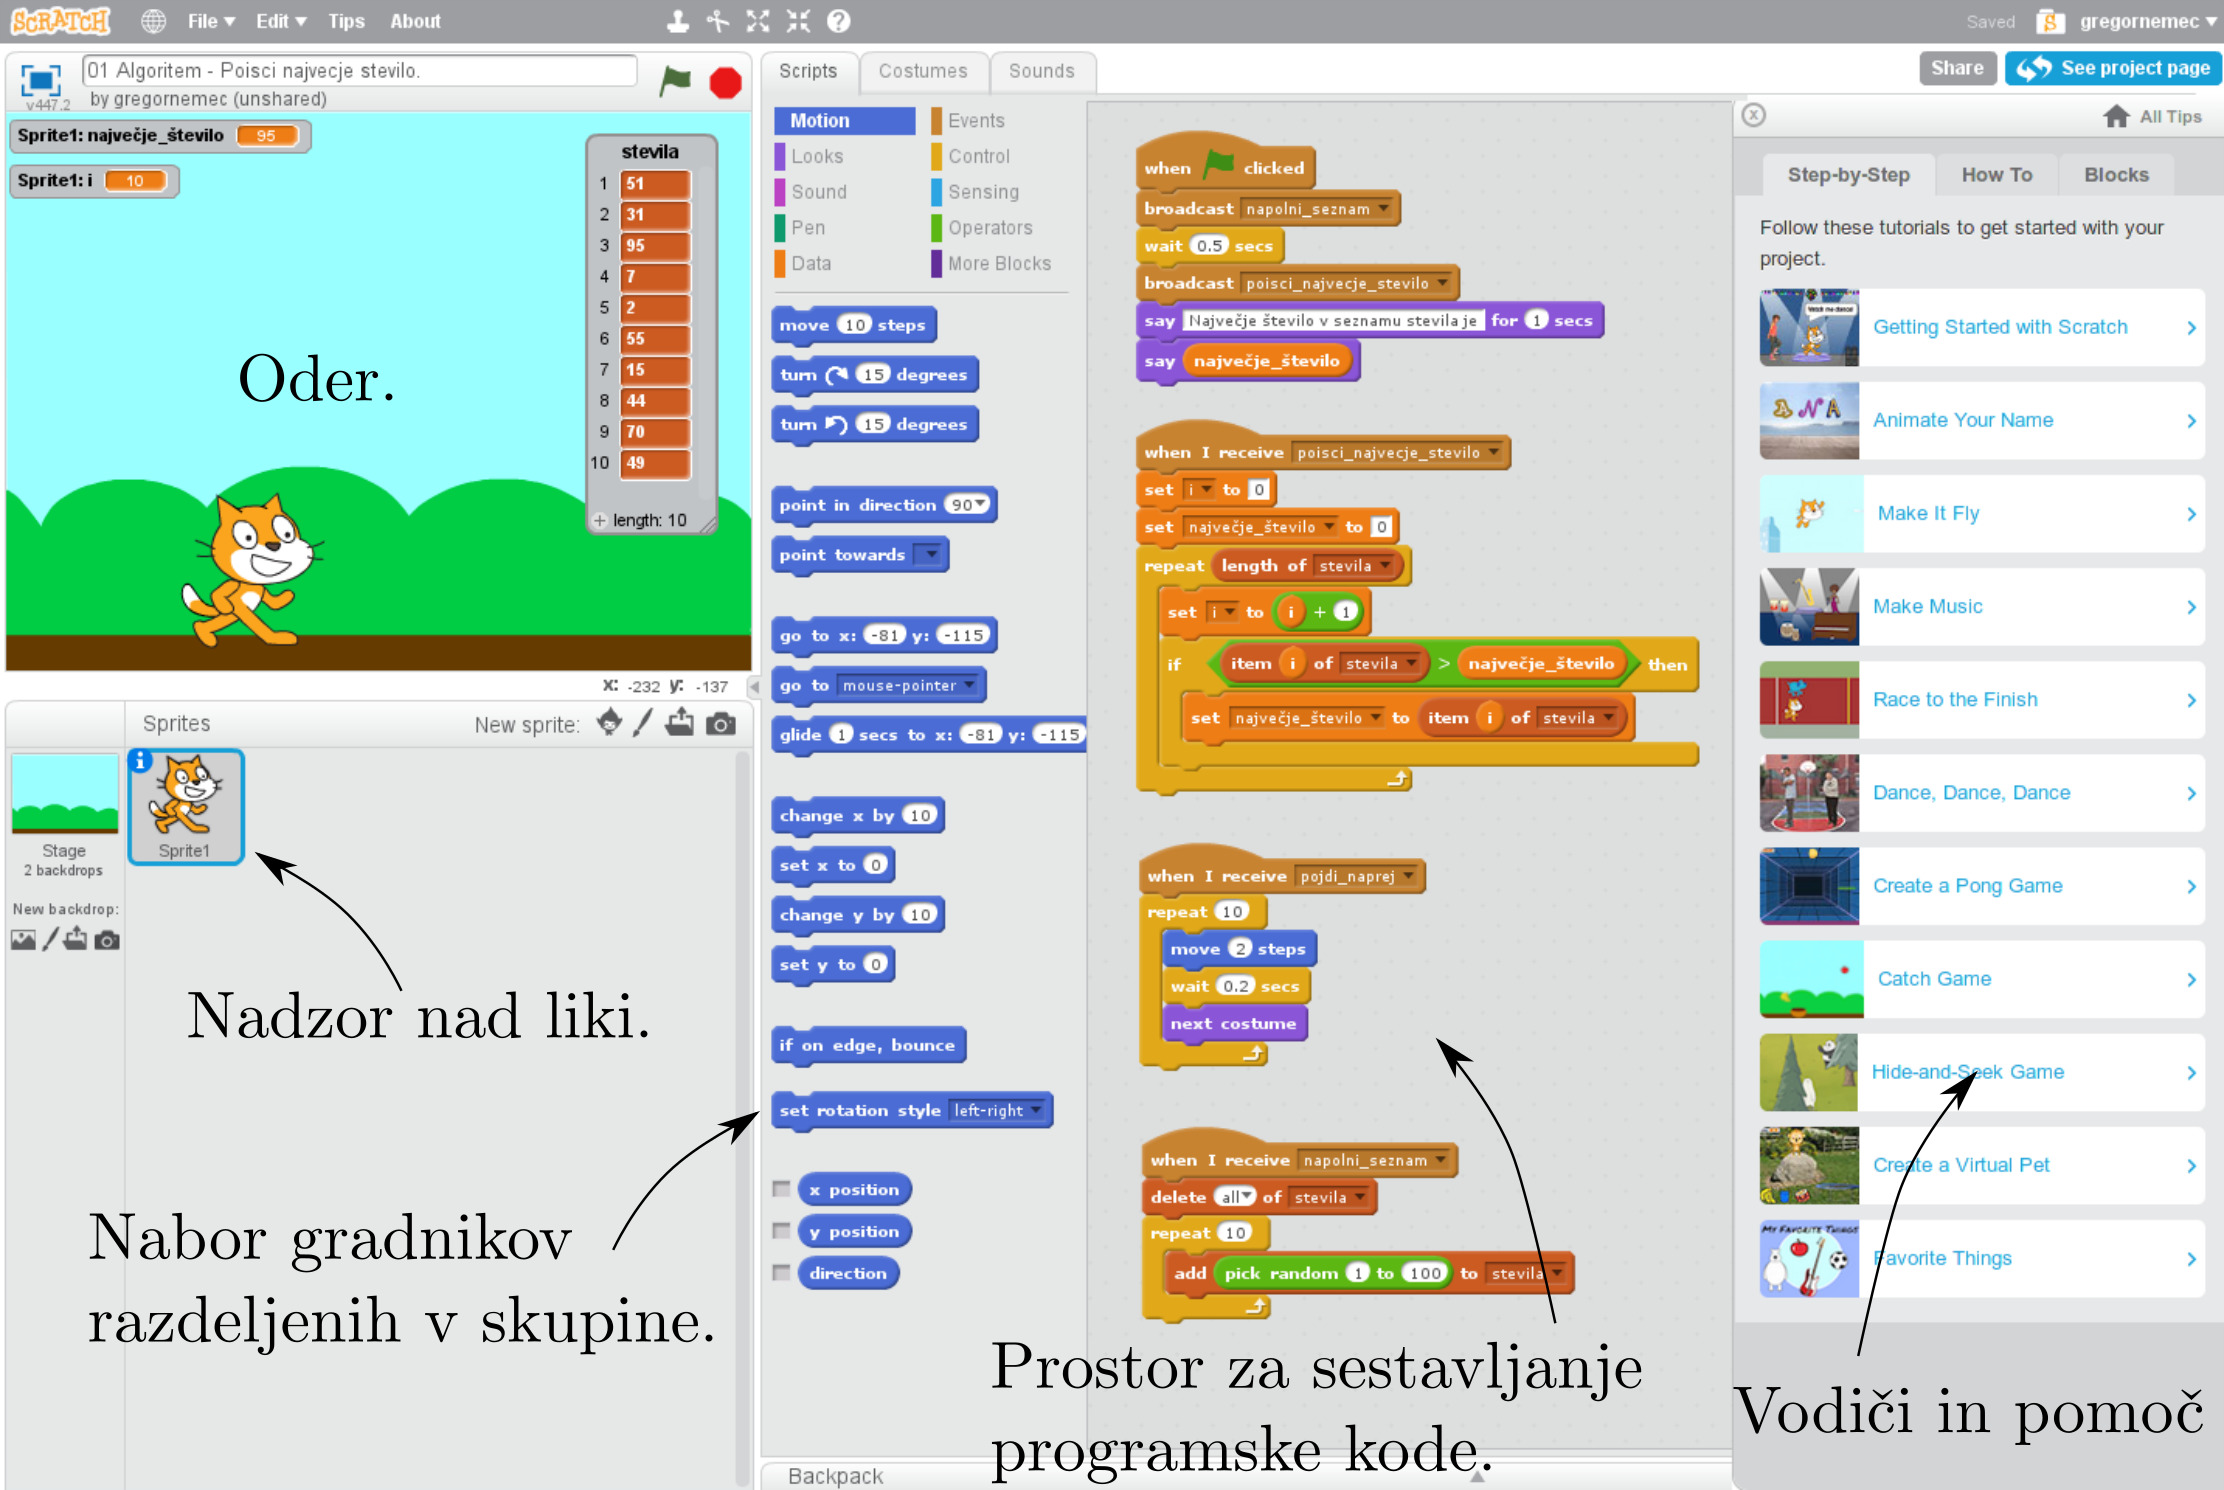
\includegraphics [width=0.90\linewidth, keepaspectratio =
   1] {./images/sc_web/scratch_orodje-v021.jpg}
   \caption{Zaslonska slika
     \emph{\href{https://scratch.mit.edu/}{Scratch}}
     \cite{web:scratch}.}
    \label{fig:web:scratch:orodje}
\end{figure}

\textbf{Vodiče} v Scratchu najdemo na desnem robu (slika
\ref{fig:web:scratch:orodje}). Vodiči so sestavljeni tako, da
uporabnika postopoma vodijo skozi gradnjo programa. S tem je
zagotovljena \textbf{postopnost}. Posamezen korak v vodiču je
sestavljen iz besedila in animiranega poteka dela.

\subsubsection{Deljenje in raziskovanje projektov}
\label{sec:deljenje_vsebin}

Vsak uporabnik, ki se registrira na spletnem portalu, ima dostop do
svojega profila. Na svoji strani se samodejno shranjujejo projekti, ki
smo jih izdelovali in jih od tu lahko ponovno naložimo za
urejanje. Vse projekte lahko delimo z drugimi. Vsak projekt ima svojo
podstran, na kateri določamo nastavitve za \emph{deljenje} (slika
\ref{fig:web:scratch:deljenje}). Na strani lahko dodamo \emph{navodila
  za program} in \emph{zapiske in zasluge}, prav tako določamo, če
želimo projekt deliti ali ne.

\begin{figure}[h!]
  \centering
    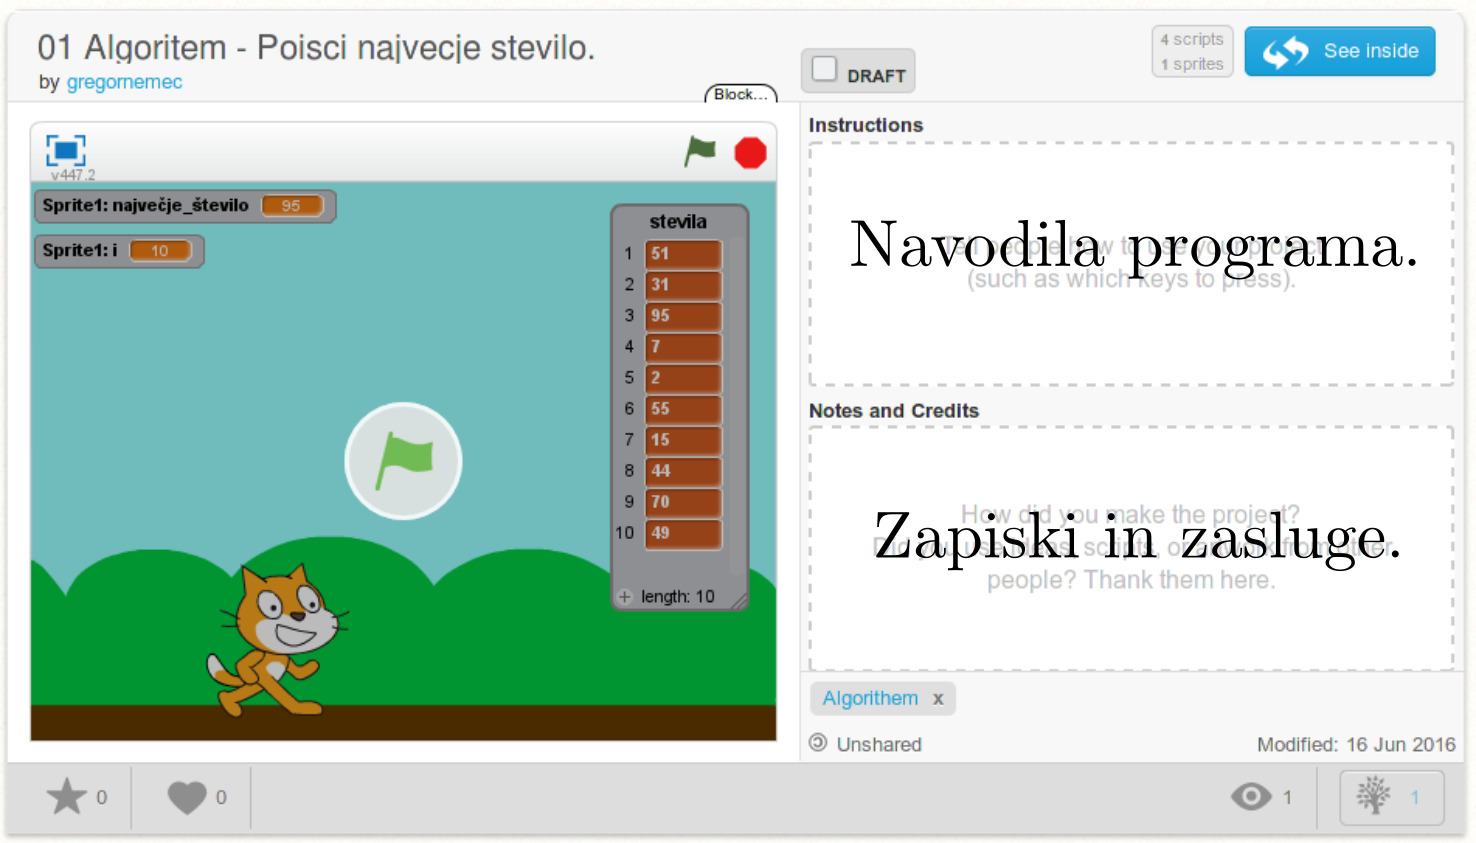
\includegraphics [width=0.50\linewidth, keepaspectratio =
   1] {./images/sc_web/scratch_deljenje-v01o.jpg}
   \caption{Podstran za deljenje projekta na
     \emph{\href{https://scratch.mit.edu/}{Scratchu}}
     \cite{web:scratch}.}
    \label{fig:web:scratch:deljenje}
\end{figure}

Če je omogočeno, da lahko delimo vsebine, je na spletnem portalu tudi
dobro poskrbljeno za \textbf{raziskovanje projektov} drugih
uporabnikov. Pod zavihkom \emph{razišči (ang. Explor)} najdemo
številne projekte, ki so razporejeni v kategorije. Tu lahko črpamo
številne ideje in si najljubše projekte shranimo tudi na svojem
profilu.

\subsubsection{Povzetek}
\label{sec:scratch_povzetek}

\textbf{Učni načrt} v slovenski osnovni šoli neobveznega izbirnega
predmeta \textbf{računalništvo} je prilagojen prav za uporabo
Scratcha, kot je razvidno iz ciljev. Čeprav z dobro pripravljenimi
vodiči spoznavamo tudi na primer vejitve, si mora učitelj pripraviti
in prilagoditi vsebino za uresničevanja učnega načrta sam. Kot smo že
lahko ugotovili, na spletu in na sploh ne zmanjka literature in idej,
ki učitelju pomagajo pri uresničevanju učnega načrta s Scratchem. Tudi
na spletni strani Scratcha lahko črpamo številne ideje iz projektov
drugih uporabnikov.

Za slabost spletne različice štejemo, da je narejen z zaprto
tehnologijo \textbf{Adobe Flash}, kar pomeni, da si mora uporabnik 
naložiti vtičnik Flash za spletni brskalnik. Vtičnik Flash uradno
podpira le nekatere komercialne operacijske sisteme in njegovo vlogo
zamenjuje vedno boljše zmožnosti samih spletnih brskalnikov s
tehnologijo \textbf{HTML5 + CSS + JS}.

\begin{osebnabox}[label={osebna:scratch}]{Scratch | \url{https://scratch.mit.edu}}
    \begin{tabular}{
  p{0.30\linewidth-2\tabcolsep} |
  p{0.70\linewidth-2\tabcolsep}  }
  \textbf{Vrsta vsebine} & Spletna aplikacija za prog. \\
      \hline
  \textbf{Jezik spletne strani} & Scratch: angleščina: da, slovenščina: da,
                                  drugi: da. Spletni portal:
                                  angleščina: da, drugi: ne.\\
      \hline
  \textbf{Ponujena znanja} & Vodiči za spoznavanje uporabe Scratch in pomoč. \\
      \hline
 \textbf{Programski jeziki} & Scratch. \\
      \hline
  \textbf{Težavnostna stopnja} & Osnovna šola. \\
      \hline
   \textbf{Upoštevanje načel} & Problemski pristop: ne,
                                sistematičnost: ne, postopnost: da (vodič). \\
      \hline
  \textbf{Dosežki/Gamification} & Ne. \\
      \hline
  \textbf{Dodajanje lastnih vsebin} & Da, vendar v smislu ustvarjanja
                                      lastnih projektov in ne
                                      celovitih vadnic. \\
      \hline
  \textbf{Upravljanje razreda} & Ne. \\
      \hline
  \textbf{Dostop vsebin} & Brezplačen. \\
\end{tabular}
\end{osebnabox}

\subsection{Repl.it}
\label{sec:repl.it}

\textbf{\emph{\href{https://repl.it/}{Repl.it}}} \cite{web:replIT} je še ena
\textbf{spletna aplikacija za programiranje}. Podjetje, ki spletno
stran ustvarja, je tržno osredotočeno na ponujanje \textbf{aplikacijskega
  programskega vmesnika - APV} ali (\emph{ang. application programming
  interface - \textbf{API}}). Njihov APV uporabljajo številni spletni
portali, kot je na primer
\emph{\href{freecodecamp}{https://www.freecodecamp.com}}
\cite{web:freecodecamp} in nekateri drugi plačljivi spletni
portali. Na svoji strani ponujajo prost dostop do spletne aplikacije
za programiranje (slika \ref{fig:web:replIT}).

\begin{figure}[h!]
  \centering
    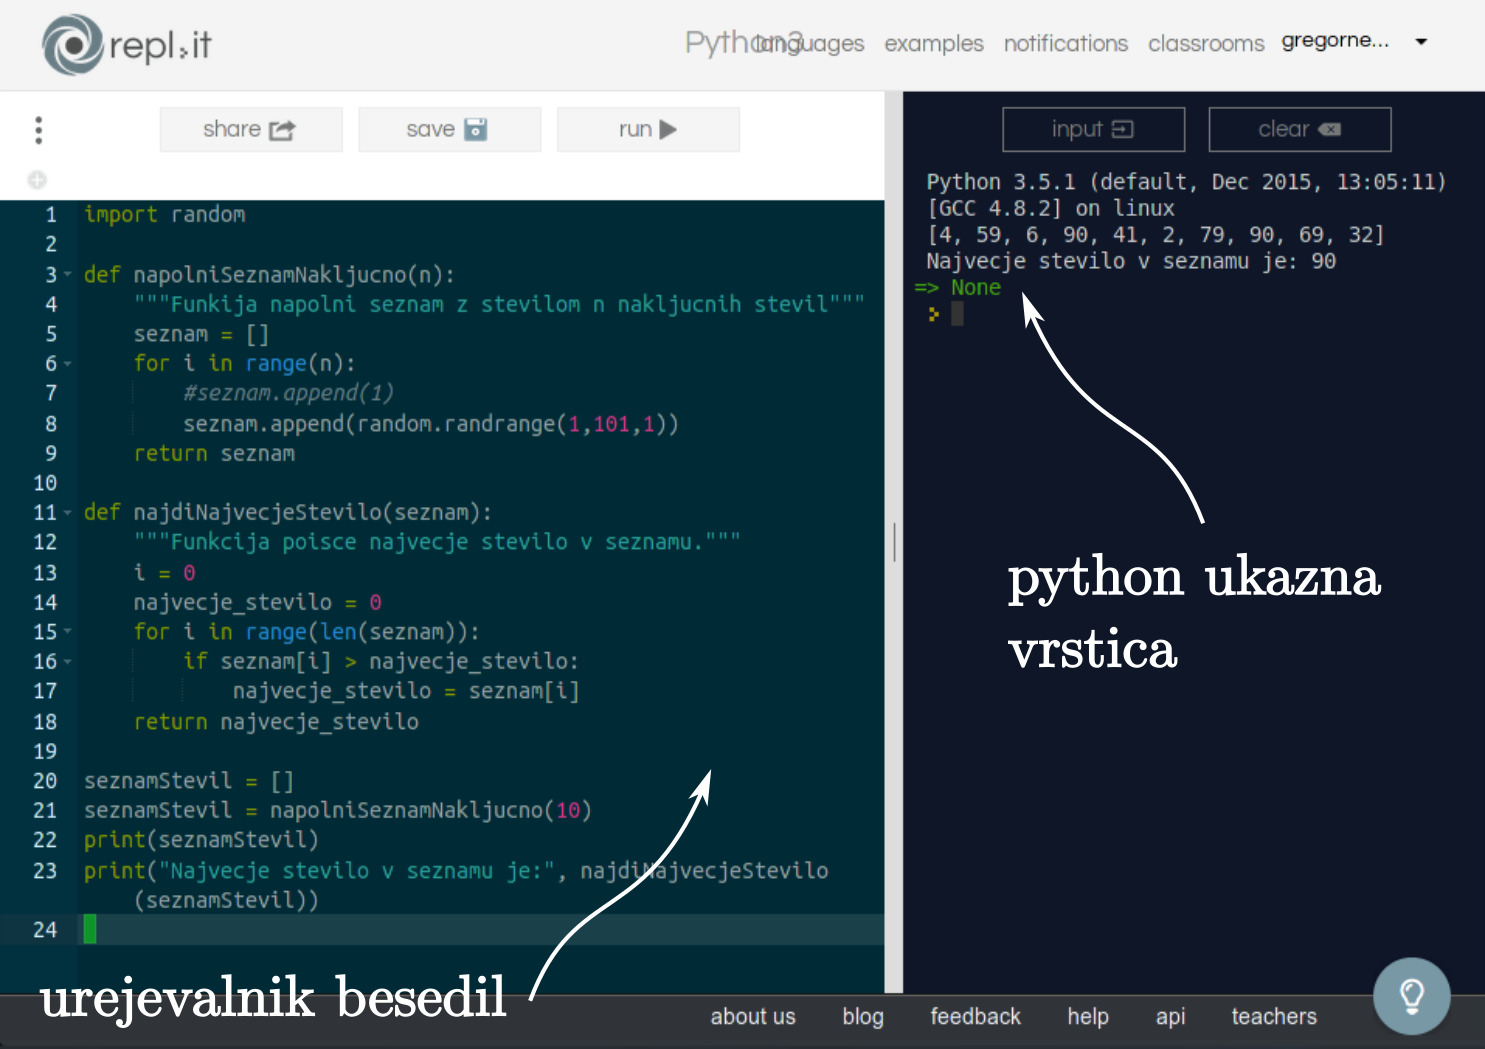
\includegraphics [width=0.65\linewidth, keepaspectratio =
   1] {./images/sc_web/replIT_main-v01.jpg}
   \caption{Zaslonska slika spletne aplikacije za programiranje
     \emph{\href{https://repl.it/}{repl.it}} \cite{web:replIT}.}
    \label{fig:web:replIT}
\end{figure}

Aplikacija ponuja številne programske jezike, kot je \textbf{Python3,
  Ruby, JavaScript, HTML, CSS, C\#, JAVA} in še mnoge druge. Vsaka nova
pojava spletne aplikacije predstavlja novo sejo. Po registraciji na
spletnem portalu lahko shranjujemo posamezne seje. Posamezno sejo
lahko \textbf{tudi delimo} preko spletne povezave. \textbf{Urejevalnik
  besedil} omogoča barvanje rezerviranih besed programske kode in ima napredno
\textbf{možnost ponujanja predlogov} za samodokončanje izpisa
rezerviranih besed in funkcij programskega jezika.

\subsubsection{Ustvarjanje razredov in nalog}
\label{sec:ustvarjanje_raz_nalog}

Spletni portal skoraj da ni vreden omembe z \textbf{vsebinskega
  vidika}, tudi kot spletna aplikacija ne predstavlja nekih posebnih
funkcij, ki jih ne bi imele tudi nekatere druge spletne aplikacije. Ima
pa spletni portal veliko zmožnost, saj omogoča \textbf{ustvarjanje
  razredov}. Mentor lahko ustvari razred in v njega povabi dijake ter
samodejno dodaja oz. \textbf{ustvarja lastne naloge}
oz. \textbf{vadnice} (slika \ref{fig:web:replIT:assigment}). Dijake v
razred povabi z dodajanjem elektronskih naslovov v seznam. Dijakom ni potrebna
registracija. S povezavo, ki so jo dobili na elektronski naslov, se prijavijo v
razred. Mentor v načinu ustvarjanja naloge doda lastna navodila in
začetno programsko kodo. V naslednjem koraku se mentor lahko odloči,
ali bo pravilnost naloge preverjal sam ali bo dodal samodejni
preizkus programske kode. V samodejnem načinu mora podati primer
vhodnih podatkov in rezultat izhoda.

V razredu imajo dijaki vpogled v seznam nalog. Naloge so dijakom
prikazane z navodili. Dijaki rešujejo nalogo, in ko so zadovoljni s
svojo rešitvijo, nalogo oddajo. Mentorju se status naloge pri dijaku
spremeni na \emph{oddano} in sedaj lahko mentor nalogo pregleda, poda
komentar in jo označi kot \emph{opravljeno} ali jih s sporočilom tudi
\emph{zavrne}.

\begin{figure}[h!]
  \centering
    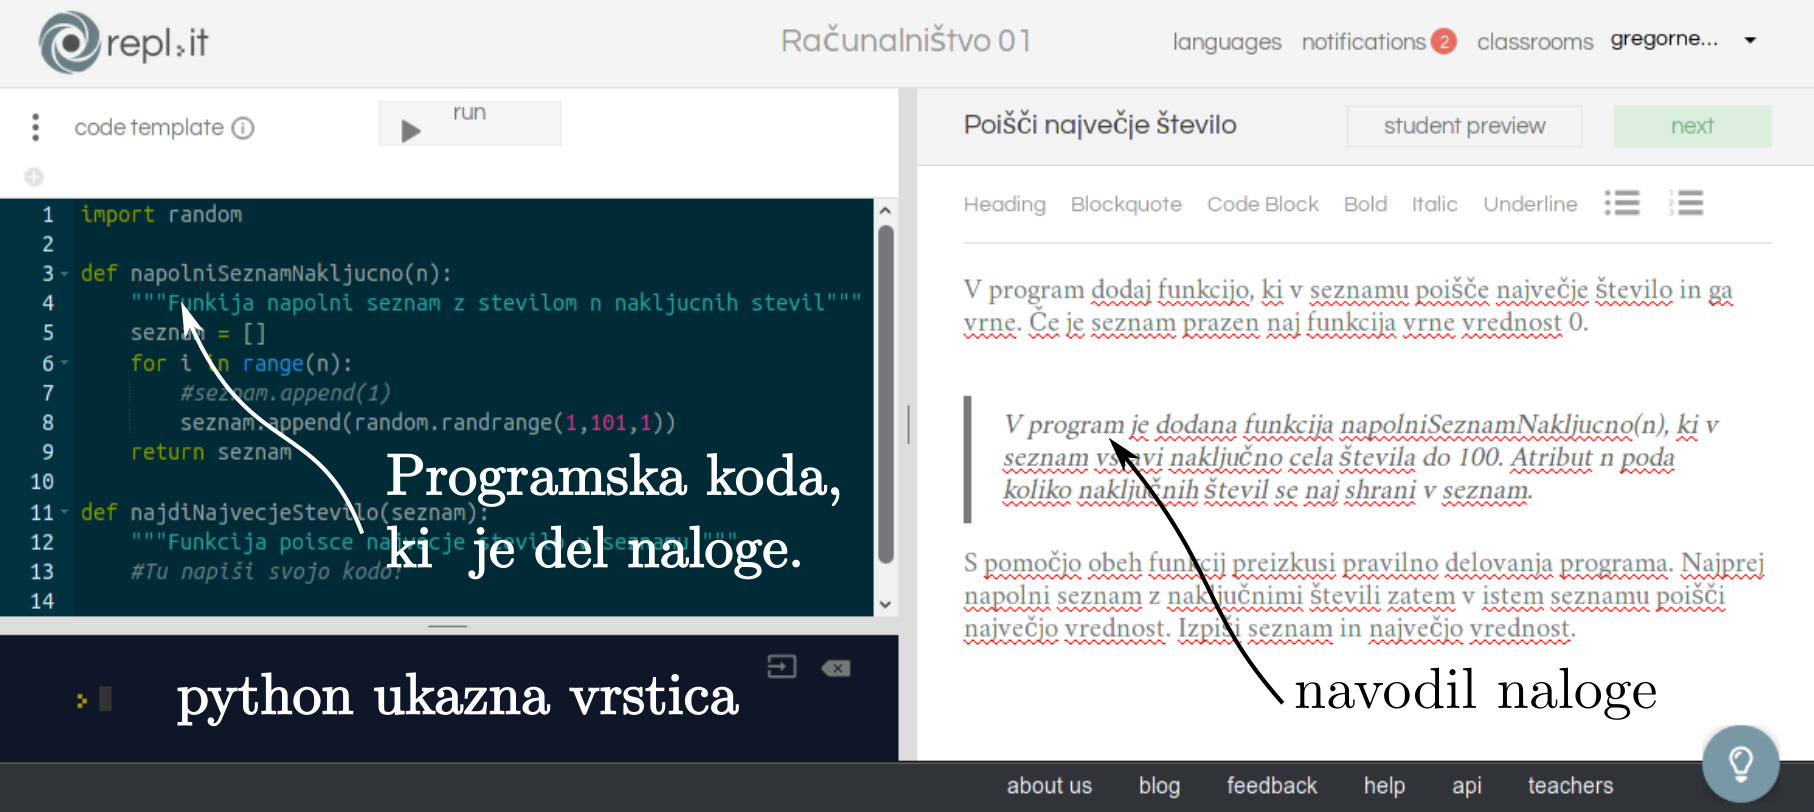
\includegraphics [width=0.65\linewidth, keepaspectratio =
   1] {./images/sc_web/replIT_assigment-v01.jpg}
   \caption{Zaslonska slika pogleda mentorja v načinu priprave naloge
     \cite{web:replIT}.}
    \label{fig:web:replIT:assigment}
\end{figure}

\subsubsection{Povzetek}
\label{sec:povzetek:replIT}

Spletna aplikacij za programiranje ponuja mentorjem računalniških
vsebin osnovno orodje za ustvarjanje razredov in nalog ter
komunikacijo z dijaki. Pri tem uporablja osnovne zmožnosti brez
pretirane kompleksnosti. Sam spletni portal ne ponuja nobene vsebine,
kar je svojevrstna prednost, saj lahko mentor prilagodi naloge učnemu
načrtu v svojem jeziku.

\begin{osebnabox}[label={osebna:replIT}]{Repl.it | \url{https://repl.it/}}
    \begin{tabular}{
  p{0.30\linewidth-2\tabcolsep} |
  p{0.70\linewidth-2\tabcolsep}  }
  \textbf{Vrsta vsebine} & Spletna aplikacija za prog. \\
      \hline
  \textbf{Jezik spletne strani} & Angleščina: da, slovenščina: ne,
                                  drugi: ne. \\
      \hline
  \textbf{Ponujena znanja} & Ne ponuja nobene vsebine.\\
      \hline
 \textbf{Programski jeziki} & Python3,
  Ruby, JavaScript, HTML, CSS, C\#, JAVA in drugi.\\
      \hline
  \textbf{Težavnostna stopnja} & Srednja šola.\\
      \hline
   \textbf{Upoštevanje načel} & Problemski pristop: ne,
                                sistematičnost: ne, postopnost: ne (vodič). \\
      \hline
  \textbf{Dosežki/Gamification} & Ne. \\
      \hline
  \textbf{Dodajanje lastnih vsebin} & Da. Ustvarjanje razreda in nalog
                                      ter komunikacija z dijaki. \\
      \hline
  \textbf{Upravljanje razreda} & Da. \\
      \hline
  \textbf{Dostop vsebin} & Brezplačen. \\

\end{tabular}
\end{osebnabox}

\subsection{Tutorialspoint}
\label{sec:tutorials_point}

\emph{\href{http://www.tutorialspoint.com/}{Tutorials point}}
\cite{web:tutorialspoint} je eden izmed velikih portalov, ki ponujajo
obsežne in zahtevne vodiče tehničnih in netehničnih vsebin. Na
spletu je vodičev veliko, tega smo izpostavili, ker ponuja
ogromno \textbf{vsebin programiranja in računalniške znanosti}, vsi
primeri v vodičih imajo \textbf{možnost preizkusa} in imajo razvito 
lastno \textbf{spletno aplikacijo za programiranje}, ki ima veliko
zmožnosti, nekatere značilne za namizne \textbf{IDE}.

Spletni portal ponuja knjižnico vodičev (\ref{fig:web:tutpoint:lib})
različnih vsebinskih sklopov. S slike je razvidno, da je zares
obsežna.

\begin{figure}[h!]
  \centering
    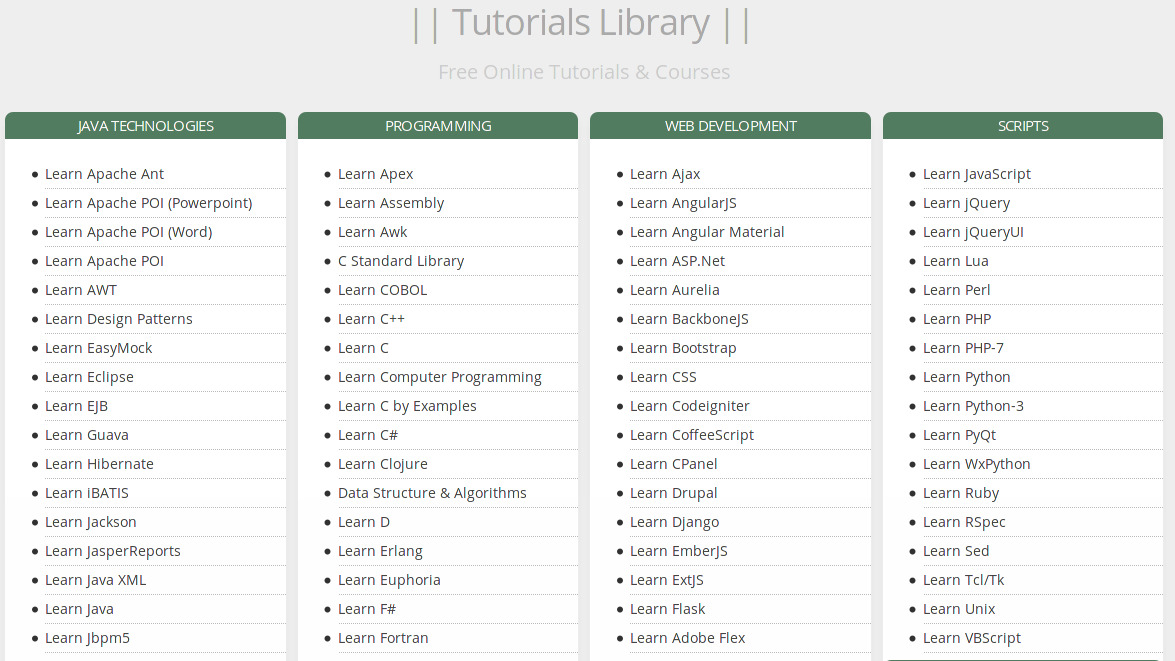
\includegraphics [width=0.65\linewidth, keepaspectratio =
   1] {./images/sc_web/tutpoint_lib-v01.jpg}
   \caption{Del seznama oz. knjižnica vodičev, ki ga ponuja spletna
     stran \emph{\href{http://www.tutorialspoint.com/}{Tutorials
         point}} \cite{web:tutorialspoint}.}
    \label{fig:web:tutpoint:lib}
\end{figure}

Vsebinsko smo si pregledali vodič za \textbf{Python3} (slika
\ref{fig:web:tutpoint:tut01}). Vodiči so oblikovani tako, da na desni
strani najdemo kazalo vsebine, v sredinskem delu je razložena snov s
primeri.

%Dodaj besedilo v sliko.
\begin{figure}[h!]
  \centering
    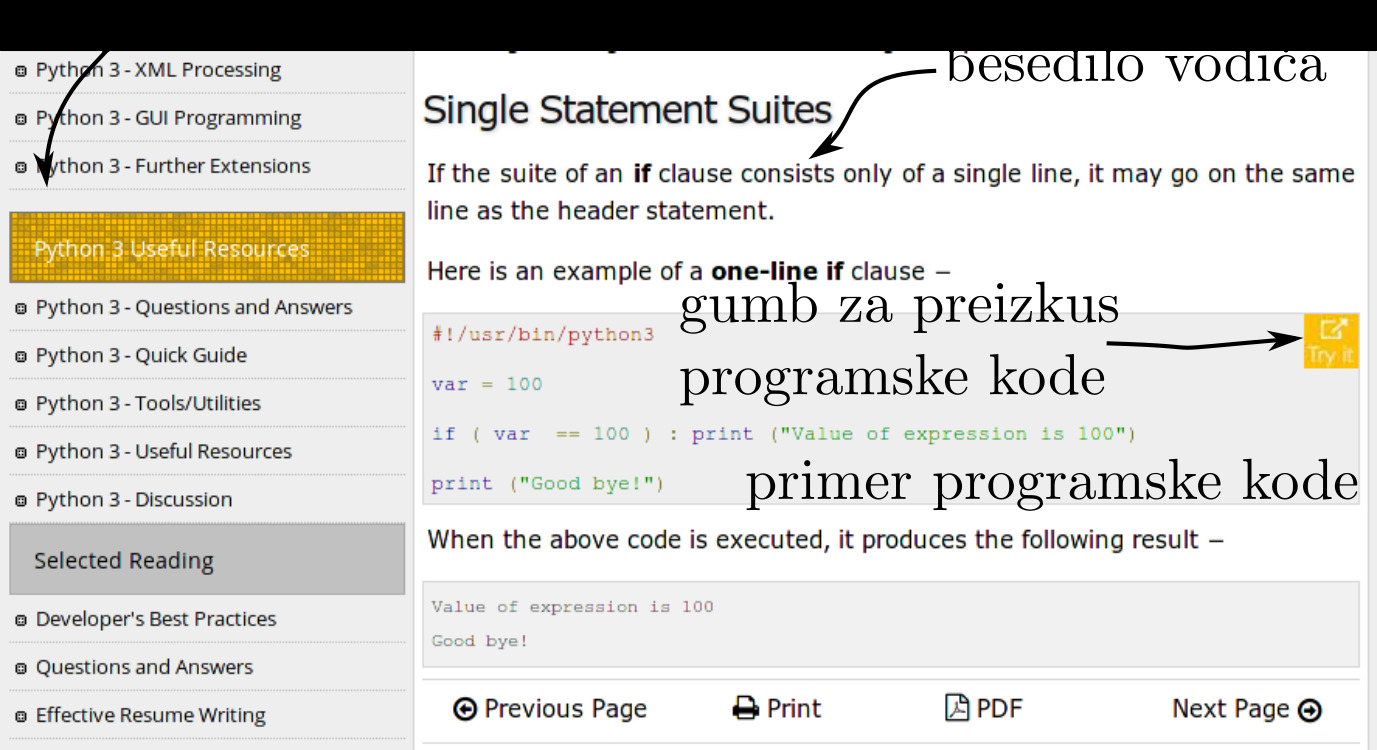
\includegraphics [width=0.65\linewidth, keepaspectratio =
   1] {./images/sc_web/tutpoint_tutP3-v01.jpg}
   \caption{Zaslonski izrez vodiča za Python3. S slike je razvidno
     kazalo in gumb za \textbf{preizkus} \cite{web:tutorialspoint}.}
    \label{fig:web:tutpoint:tut01}
\end{figure}

Nekatere od primerov lahko tudi preizkusimo, s klikom na gumb
\textbf{preizkusi (\emph{ang. Try it})} se nam na isti strani odpre
podokno (slika \ref{fig:web:tutpoint:tut02}). Kodo v urejevalniku
lahko spreminjamo in ponovno zaženemo.

%Dodaj besedilo v sliko.
\begin{figure}[h!]
  \centering
    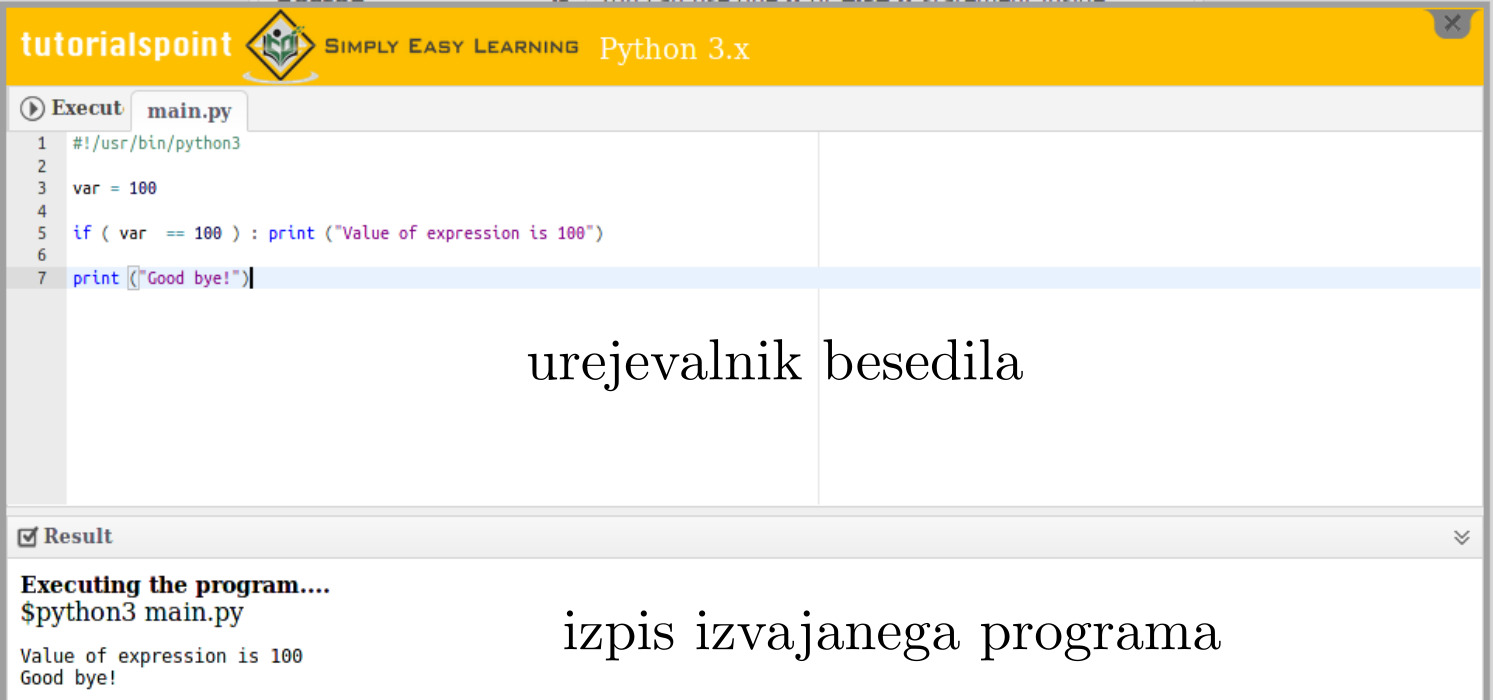
\includegraphics [width=0.65\linewidth, keepaspectratio =
   1] {./images/sc_web/tutpoint_tutP3-v02.jpg}
   \caption{Podokno za preizkus primera programske kode
     \cite{web:tutorialspoint}.}
    \label{fig:web:tutpoint:tut02}
\end{figure}

\subsubsection{Coding ground}
\label{sec:coding_ground}

Kot smo že omenili, spletni portal kot orodje ponuja lastno spletno
aplikacijo za programiranje. Spletna aplikacija se imenuje
\emph{\href{http://www.tutorialspoint.com/codingground.htm}{Codingground}}
\cite{web:tutorialspoint:codingground}. Na uvodni strani orodja (slika
\ref{fig:web:tutpoint:cg-pl}) smo odkrili številnost ponujenih
\textbf{programskih jezikov}, ki sovpadajo s številnimi vodiči, ki jih
ponuja spletni portal.

\begin{figure}[h!]
  \centering
    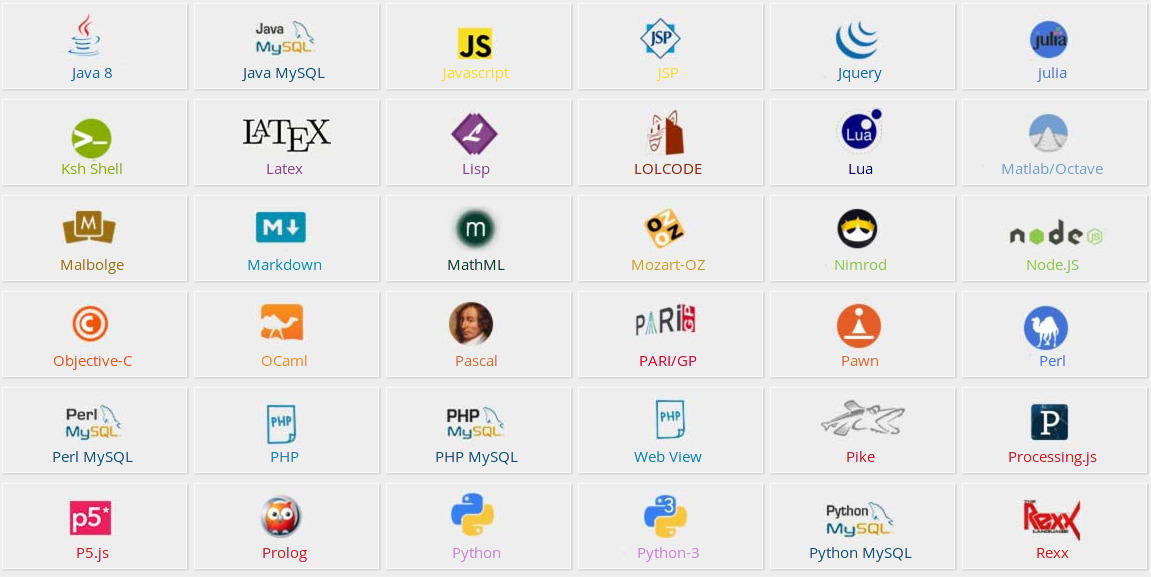
\includegraphics [width=0.65\linewidth, keepaspectratio =
   1] {./images/sc_web/tutpoint_cg-pl-v01.jpg}
   \caption{Del seznama različnih programskih jezikov, ki jih lahko
     uporabljamo s spletno aplikacijo za programiranje
     \emph{\href{http://www.tutorialspoint.com/codingground.htm}{Codingground}}
     \cite{web:tutorialspoint:codingground}.}
    \label{fig:web:tutpoint:cg-pl}
\end{figure}

Razporeditev spletne aplikacije (slika \ref{fig:web:tutpoint:cg}) je
taka, da imamo na levem robu seznam datotek v korenskem imeniku, v
sredinskem delu je urejevalnik besedil, nad urejevalnikom najdemo
menijsko vrstico in na dnu strani je \textbf{ukazna vrstica}, v kateri
lahko zaganjamo napisano programsko kodo. V njej se izpisujejo tudi
povratne informacije tolmača in izhod programske
kode. \textbf{Urejevalnik besedil} omogoča barvanje kode
rezerviranih besed in nastavljanje barvne sheme
urejevalnika. Urejevalnik omogoča še samodejno zamikanje programske
kode, ko je to potrebno. \textbf{Shranjevanje in uvažanje projektov v
  oblak} lahko smatramo kot eno izmed večjih zmožnosti te spletne
aplikacije. \emph{\href{http://www.tutorialspoint.com/codingground.htm}{Codingground}}
lahko nastavimo, da se poveže z oblačnimi shrambami, kot so
\textbf{Dropbox, Google Drive, Onedrive}, in s sistemom za objavljanje,
upravljanje različic in kolaboracijo \textbf{Git}. Seveda lahko projekt
naložimo neposredno z računalnika in ga tja tudi
shranimo. Prednost oblačnega shranjevanja je ta, da lahko programiramo od kjerkoli in s katerimkoli orodjem želimo - spletno
ali namizno aplikacijo. Spletna aplikacija omogoča tudi upravljanje z
datotekami. Lahko ustvarimo, preimenujemo in brišemo datoteke ali
imenike. To lahko počnemo iz \textbf{menija (\emph{file}) ali ukazne
  vrstice}. Vsak projekt lahko delimo preko neposredne kratke
\textbf{url povezave}, kot smo to že videli pri drugih spletnih
portalih.

\begin{figure}[h!]
  \centering
    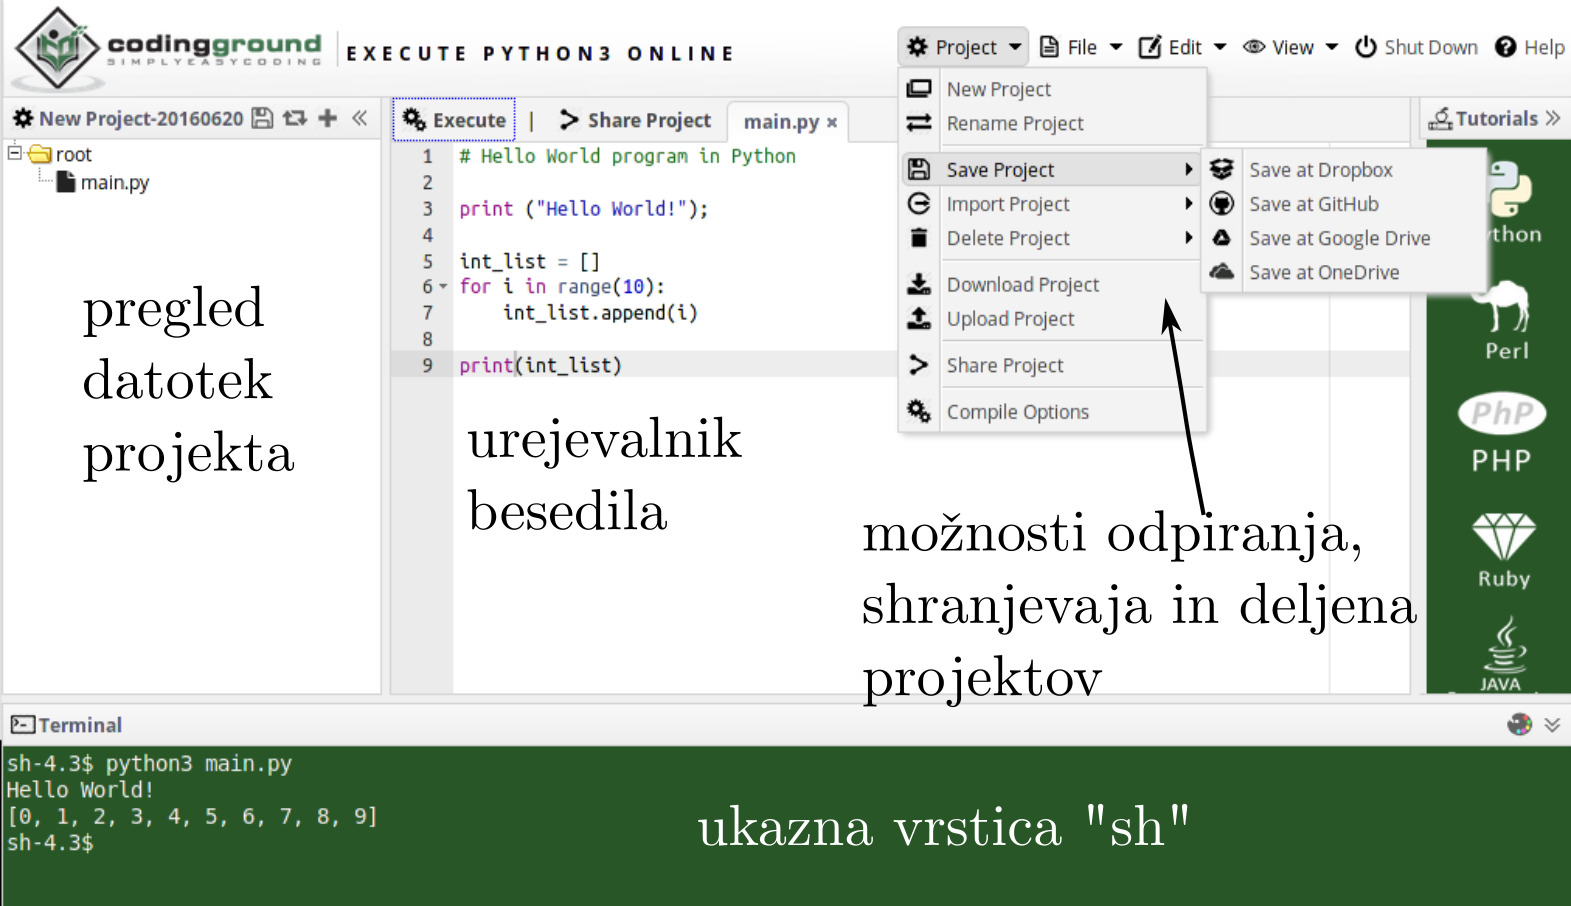
\includegraphics [width=0.65\linewidth, keepaspectratio =
   1] {./images/sc_web/tutpoint_cg-v01.jpg}
   \caption{Spletna aplikacija za programiranje -
     \emph{\href{http://www.tutorialspoint.com/codingground.htm}{Codingground}}
     \cite{web:tutorialspoint:codingground}.}
    \label{fig:web:tutpoint:cg}
\end{figure}

\subsubsection{Povzetek}
\label{sec:povzetek_tutpoint}

Vsebina vodičev je zelo tehnična in deluje kot okrnjen povzetek uradne
reference za določen programski jezik. Kot taka je predvsem primerna
za programerje začetnike, ki se želijo poučiti o določenem programskem
jeziku, vendar že poznajo osnovne koncepte programiranja. Velik plus
je preizkus programske kode. Vodiče lahko priporočimo kot
skrajšano različico reference programskemu jeziku.

S pravo nastavitvijo spletna aplikacija omogoča, da imajo dijaki
programsko kodo in snov, ki jo v nekem trenutku predelujejo, povsod na
voljo. S pomočjo shranjevanja in deljenja projektov lahko mentor
uporabi spletno aplikacijo kot glavno orodje za učenje računalništva
in programskega jezika. Mentor mora pripraviti sistem za izmenjavo
navodil, programske kode in rešitev dijakov. To lahko stori z uporabo
kratkih url povezav. Urejevalnik besedil bi lahko ponujal kakšno
zmožnost več, kot jo, vendar zadosti osnovnim potrebam pisanja
programske kode.


\begin{osebnabox}[label={osebna:tutorails point}]{Tutorialspoint |
    \url{http://www.tutorialspoint.com/}}
    \begin{tabular}{
  p{0.30\linewidth-2\tabcolsep} |
  p{0.70\linewidth-2\tabcolsep}  }
  \textbf{Vrsta vsebine} & Osnovna kombinirana vsebina: vodič in
                           preizkus programske kode. Posebej spletna
                           aplikacija za učenje programiranja:
                           Codingground. \\
      \hline
  \textbf{Jezik spletne strani} & Angleščina: da, slovenščina: ne,
                                  drugi: ne. \\
      \hline
  \textbf{Ponujena znanja} & Znanja prog. jezikov + druge
                             vsebine. Vodiči s številnih področij. \\
      \hline
 \textbf{Programski jeziki} & Velika knjižnica prog. jezikov. \\
      \hline
  \textbf{Težavnostna stopnja} & Srednja šola.\\
      \hline
   \textbf{Upoštevanje načel} & Problemski pristop: ne,
                                sistematičnost: ne, postopnost: da (vodič). \\
      \hline
  \textbf{Dosežki/Gamification} & Ne. \\
      \hline
  \textbf{Dodajanje lastnih vsebin} & Da. Ustvarjanje podporne
                                      programske kode v spletni
                                      aplikaciji za prog., vendar brez
                                      navodil in deljenja vsebine.  \\
      \hline
  \textbf{Upravljanje razreda} & Ne. \\
      \hline
  \textbf{Dostop vsebin} & Brezplačen. \\

\end{tabular}
\end{osebnabox}

\subsection{Thimble}
\label{sec:thimble}

%Vodič je lahko vodnik, spremeni!?

\emph{\href{https://thimble.mozilla.org/sl/}{Thimble}}
\cite{web:thimble} je spletni portal, ki ga gosti podjetje
\textbf{Mozilla}, ki izdaja spletni brskalnik
\textbf{Firefox}. Spletni portal je namenjen učenju spletnih
tehnologij \textbf{HTML, CSS} in \textbf{JavaScript}. Pripravljenih
je šest spletnih vsebin, ki jih lahko odpremo v projektu in jih
preurejamo. Največja prednost spletnega portala je spletna aplikacija
oz. orodje, v katerem urejamo projekte (slika
\ref{fig:web:thimble:webapp}).

\begin{figure}[h!]
  \centering
    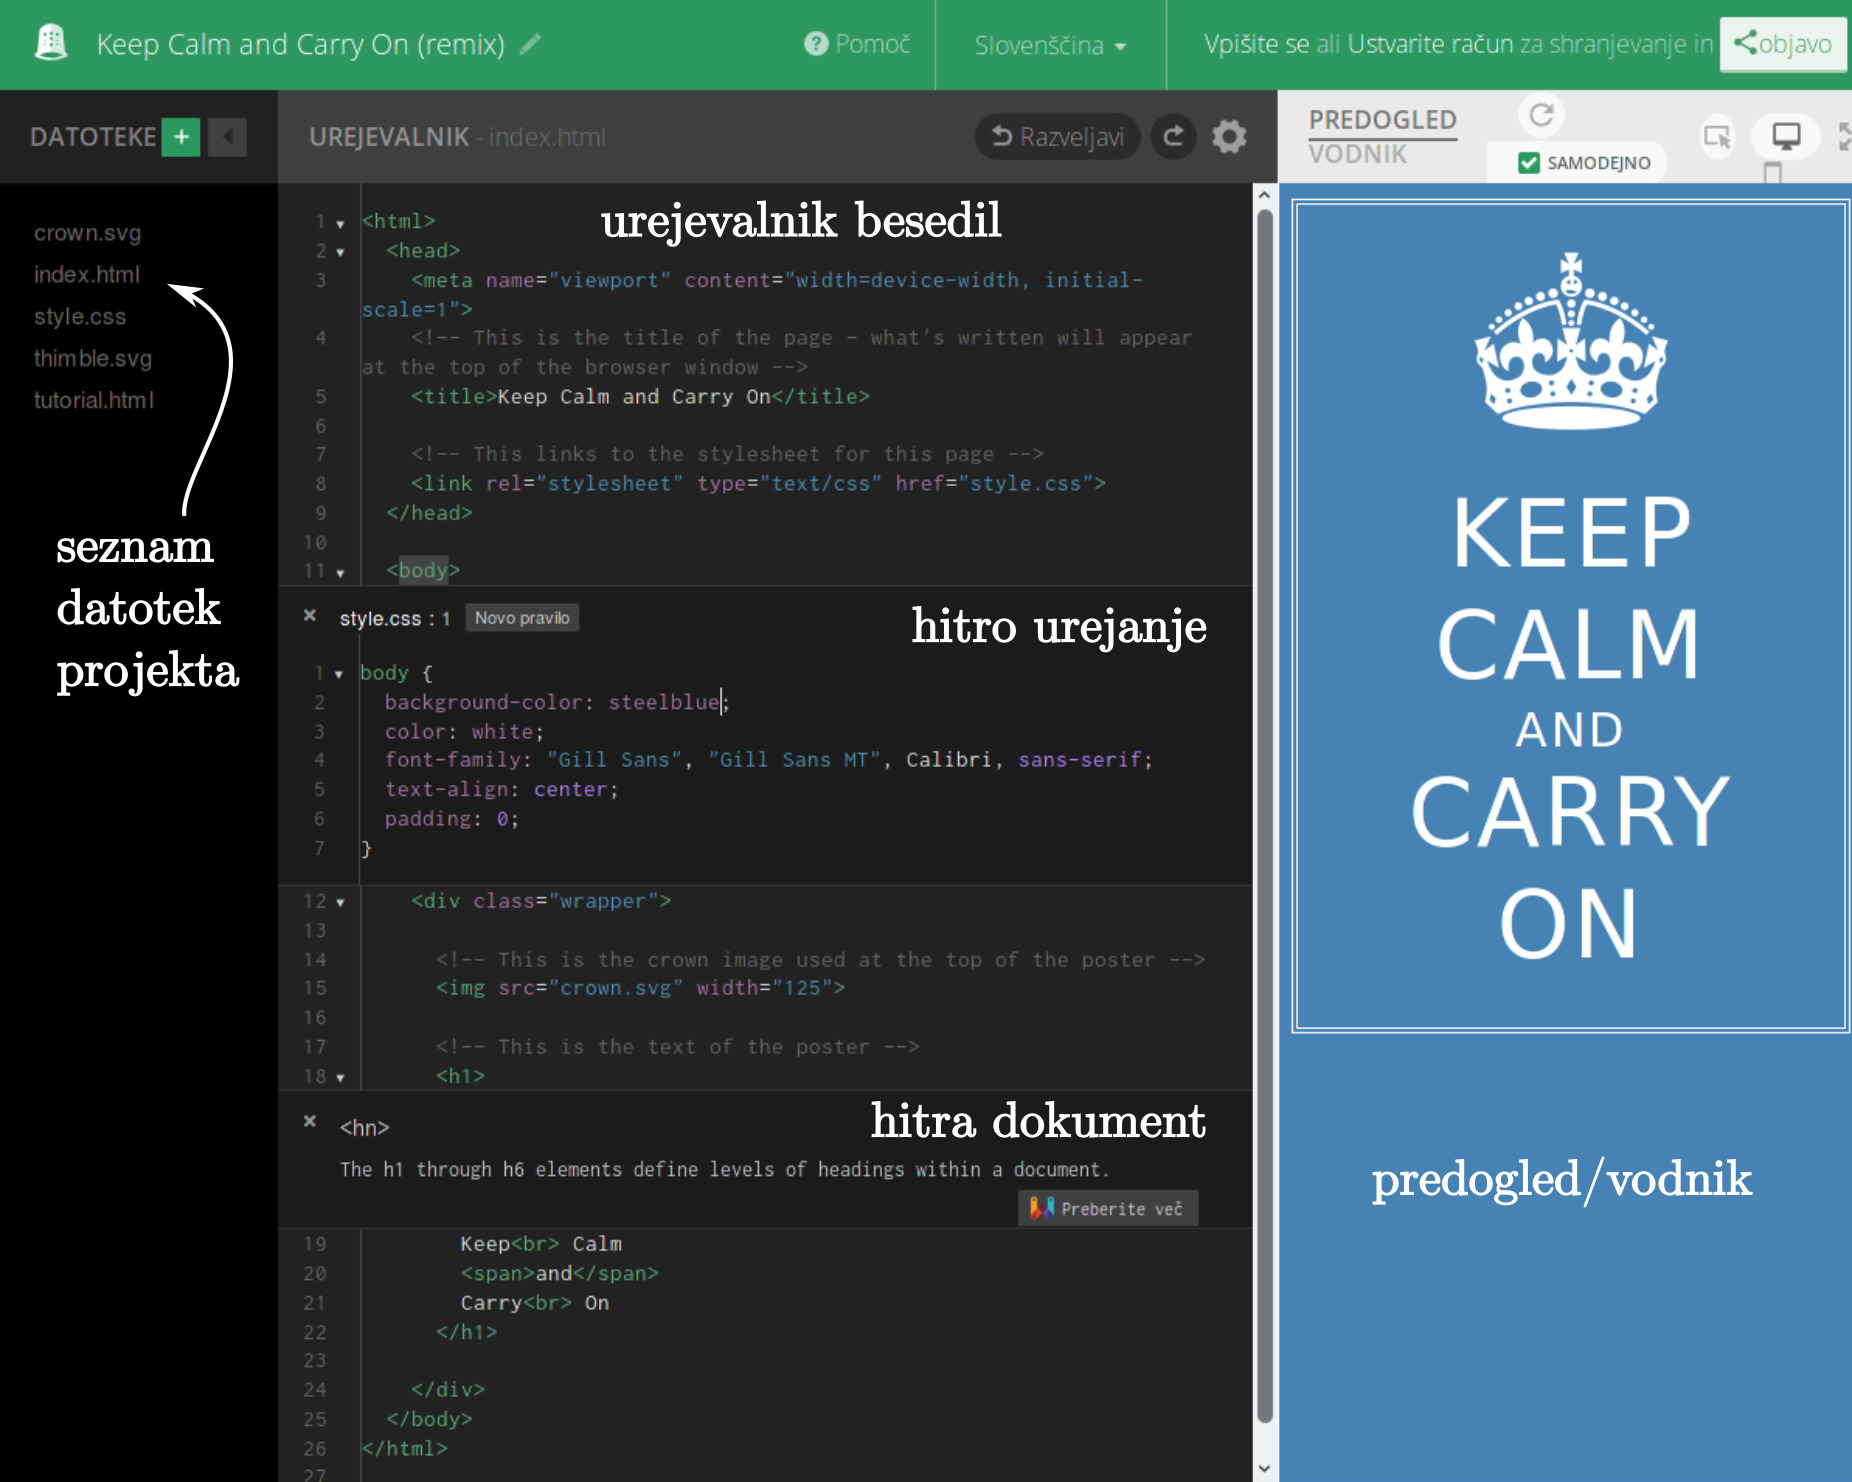
\includegraphics [width=1\linewidth, keepaspectratio =
   1] {./images/sc_web/thimble_saup-v02.jpg}
   \caption{Urejanje projekta na strani
     \emph{\href{https://thimble.mozilla.org/sl/}{Thimble}}
     \cite{web:thimble}.}
   \label{fig:web:thimble:webapp}
 \end{figure}

 Na desni strani spletne aplikacije imamo \textbf{seznam dokumentov},
 ki sestavljajo projekt. V projekt lahko dodajamo lastne dokumente.
 \textbf{Urejevalnik besedil} barva značke html in css jezika, prav
 tako upošteva barvanje besedila v primeru programskega jezika
 JavaScript. Urejevalnik ima dve priročni zmožnosti, kot je
 \emph{hitri dokument} in \emph{hitro urejanje}. Hitri dokument je
 takojšnja pomoč, ki se sproži ob pritisku kombinacije \texttt{Alt +
   K} na mestu, kjer je značka, za katero želimo dodatno razlago. Hitro
 ureja na mestu, kjer smo postavljeni v besedilu, s pritiskom
 kombinacije tipk \texttt{Alt  +E} odpre podurejevalnik s \emph{css}
 razredom, ki oblikuje značko dela html dokumenta. Funkcija hitro
 urejanje v \emph{css} dokumentu, ko smo postavljeni na barvo, pomeni
 barve z barvne palete.

 Vse spremembe, ki jih naredimo v urejevalniku, se v živo in samodejno
 posodobijo v \textbf{oknu predogleda}, ki se nahaja na levem delu. Na
 tem mestu najdemo tudi vodnika. Uvodna spletna stran in uporabniški
 vmesnik sta preveden v \textbf{slovenščino}. Žal pa vodniki, ki so
  pripravljeni na spletni strani, niso prevedeni v slovenščino.

 Če na spletni strani opravimo registracijo in se prijavimo, se nam
 spremembe na projektu shranjujejo samodejno. Projekt lahko
 preimenujemo in ga delimo z drugimi preko spletne povezave. Tisti, ki
 naš projekt odpre, ga spreminja kot lastnega in se sprememba v našem
 ne pozna. Ustvarjamo lahko tudi nove projekte, katerim dodajamo
 \texttt{html, css, js} datoteke. Dodamo lahko tudi datoteko vodiča,
 ki jo lahko poljubno spreminjamo.
 
\subsubsection{Povzetek}
\label{sec:povzetek_thimble}

Spletni portal lahko uporabljamo na vseh stopnjah. Primeren je še
posebej za uporabo v osnovni šoli pri izbirnem predmetu
\textbf{računalniška omrežja}, saj omogoča preprost in učinkovit
urejevalnik besedil. Učitelj se registrira in pripravi oz. prilagodi
obstoječi projekt za pouk. Učencem deli povezavo. Učencem se ni
potrebno registrirati in kljub temu lahko urejajo dokument kot
lasten. Učenci svoje dokončane projekte delijo kot končen izdelek s
povezavo nazaj učitelju. Na podoben način se lahko spletni portal
uporablja tudi v srednji šoli.

\begin{osebnabox}[label={osebna:thimble}]{Thimble |
    \url{https://thimble.mozilla.org}}
    \begin{tabular}{
  p{0.30\linewidth-2\tabcolsep} |
  p{0.70\linewidth-2\tabcolsep}  }
  \textbf{Vrsta vsebine} & Napredna kombinirana vsebina: vadnica
                           (vodnik + spletna aplikacija za
                           programiranje).   \\
      \hline
  \textbf{Jezik spletne strani} & Angleščina: da, slovenščina:
                                  aplikacij, da; vodnik, ne. 
                                  drugi: da. \\
      \hline
  \textbf{Ponujena znanja} & Znanje programskih jezikov, uporaba
                             spletna in spletnih vsebin. \\
      \hline
 \textbf{Programski jeziki} & HTML, CSS, JavaScript. \\
      \hline
  \textbf{Težavnostna stopnja} & Osnovna šola (3. triada) in srednja
                                 šola. \\
      \hline
   \textbf{Upoštevanje načel} & Problemski pristop: da,
                                sistematičnost: ne, postopnost: ne. \\
      \hline
  \textbf{Dosežki/Gamification} & Ne. \\
      \hline
  \textbf{Dodajanje lastnih vsebin} & Da. Možno je ustvarjanje lastnih
                                      vadnic, ki jih lahko delimo
                                      naprej.  \\
      \hline
  \textbf{Upravljanje razreda} & Ne. \\
      \hline
  \textbf{Dostop vsebin} & Brezplačen. \\

\end{tabular}
\end{osebnabox}


\subsection{Code combat}
\label{sec:code_battle}

Spletni portal \emph{\href{https://codecombat.com/}{Code combat}}
\cite{web:codecombat} je mešanica med igranjem igre in pisanjem
programske kode. V predstavitvi spletne strani pravijo naslednje:
\emph{``Če se želiš naučiti programirati, moraš napisati veliko
  programske kode.''} In poudarjajo, da oni poskrbijo, da pri tem
početju ostane zabava v ospredju \cite{web:codecombat:about}. Spletna
stran ponuja tri načine registracije, ustvarite lahko
\textbf{navaden}, \textbf{učiteljski} ali \textbf{učencev} račun. V
pregledu strani smo uporabili prijavo z navadnim računom, v
nadaljevanju smo prav tako povzeli posebnosti ostalih dveh računov.

Po registraciji in prijavi v račun si izberemo \textbf{lik in
  programski jezik}, s katerim bomo igrali (slika
\ref{fig:web:cc:hero}). Spletna igra ponuja štiri programske jezike
\textbf{Python, JavaScript, CoffeScript, LUA}. 

\begin{figure}[h!]
  \centering
    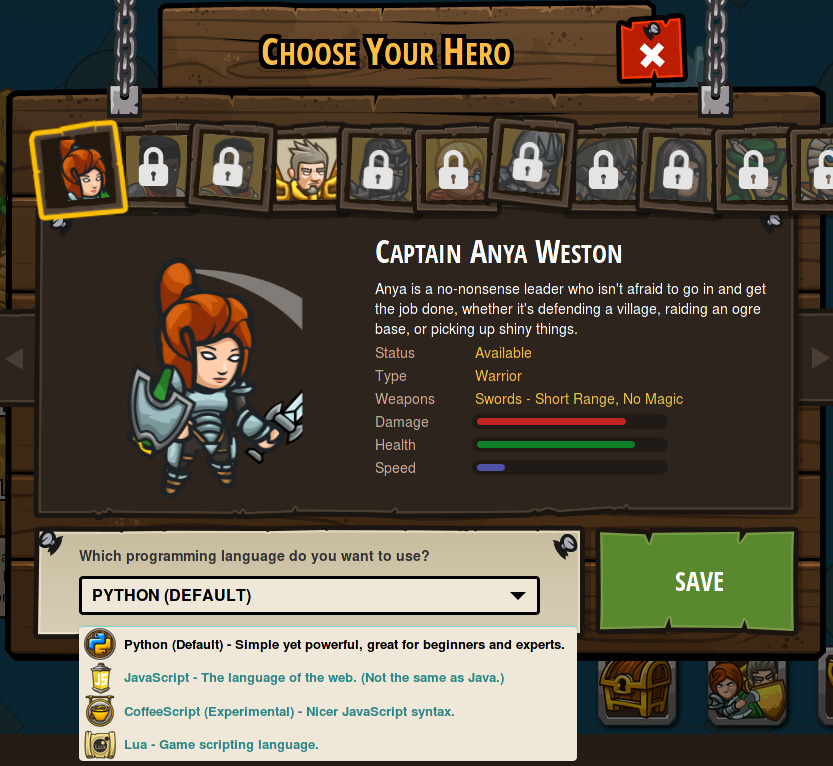
\includegraphics [width=0.45\linewidth, keepaspectratio =
   1] {./images/sc_web/cc_hero-lang-v01.jpg}
   \caption{Izbira junaka in programskega jezika \cite{web:codecombat}.}
   \label{fig:web:cc:hero}
 \end{figure}


 Po izbiri junaka preidemo na izbor \textbf{zemljevidov} (slika
 \ref{fig:web:cc:zemljevid}). Izberemo lahko samo zemljevid, ki je
 odklenjen. Druge zemljevide odklenemo tako, da rešimo vse naloge v
 njem. Posamezen zemljevid predstavlja cilje posameznih programskih
 konceptov, ki se jih uporabnik nauči, ko predela vse naloge.

\begin{figure}[h!]
  \centering
    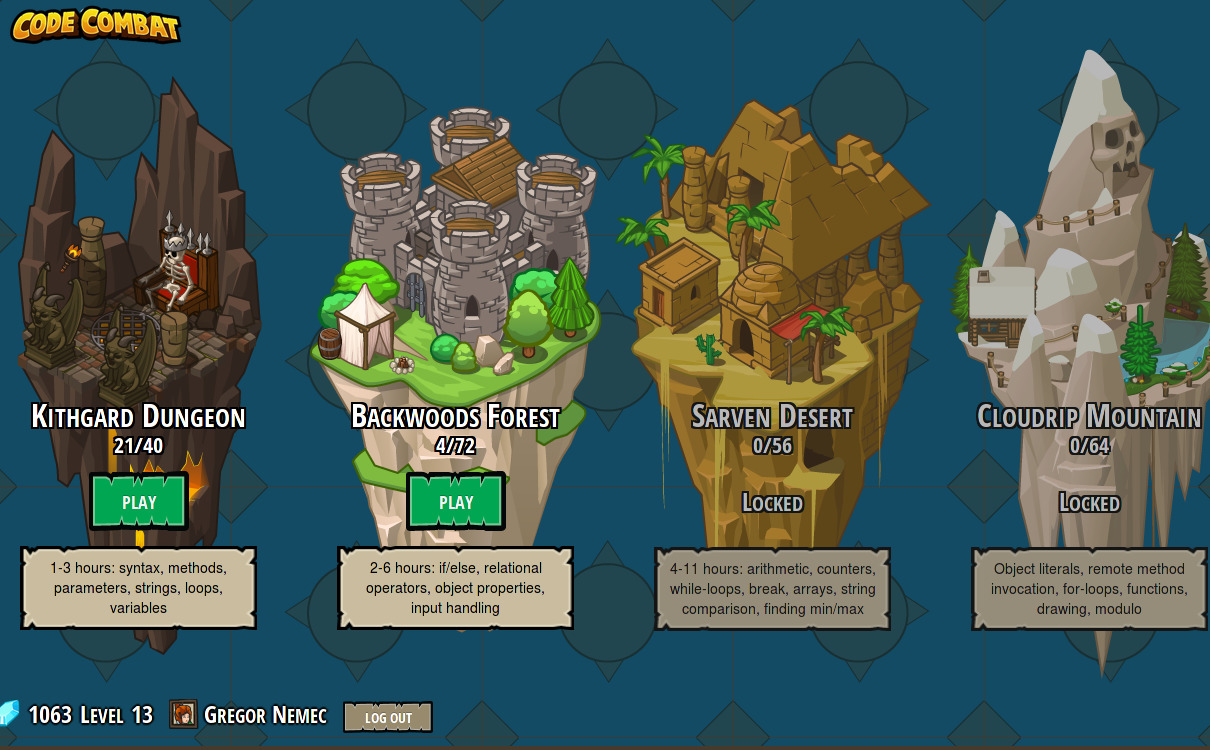
\includegraphics [width=0.65\linewidth, keepaspectratio =
   1] {./images/sc_web/cc_izbor-zem-v01.jpg}
   \caption{Izbor zemljevida, na katerem bomo reševali naloge
     \cite{web:codecombat}.}
   \label{fig:web:cc:zemljevid}
 \end{figure}

 Igra se zgleduje po tipu iger igranja vloge (\emph{ang. Role play
   game - \textbf{RPG}}). Z junakom napredujemo po zemljevidu z vsako
 opravljeno nalogo, ob koncu vsake naloge prejmemo \textbf{točke -
   izkušnje} in napredujemo v lastnih \textbf{stopnjah}. Junak nabira
 številne predmete, ki mu omogočajo nadgradnjo veščin in tako lažje
 napredovanje skozi misije. Za začetek naloge pritisnemo na rdeče
 obarvan krog na zemljevidu (slika \ref{fig:web:cc:zemljevid:BG}),
 prikaže se povzetek naloge in katere koncepte bomo uporabili pri
 reševanju naloge. 

\begin{figure}[h!]
  \centering
    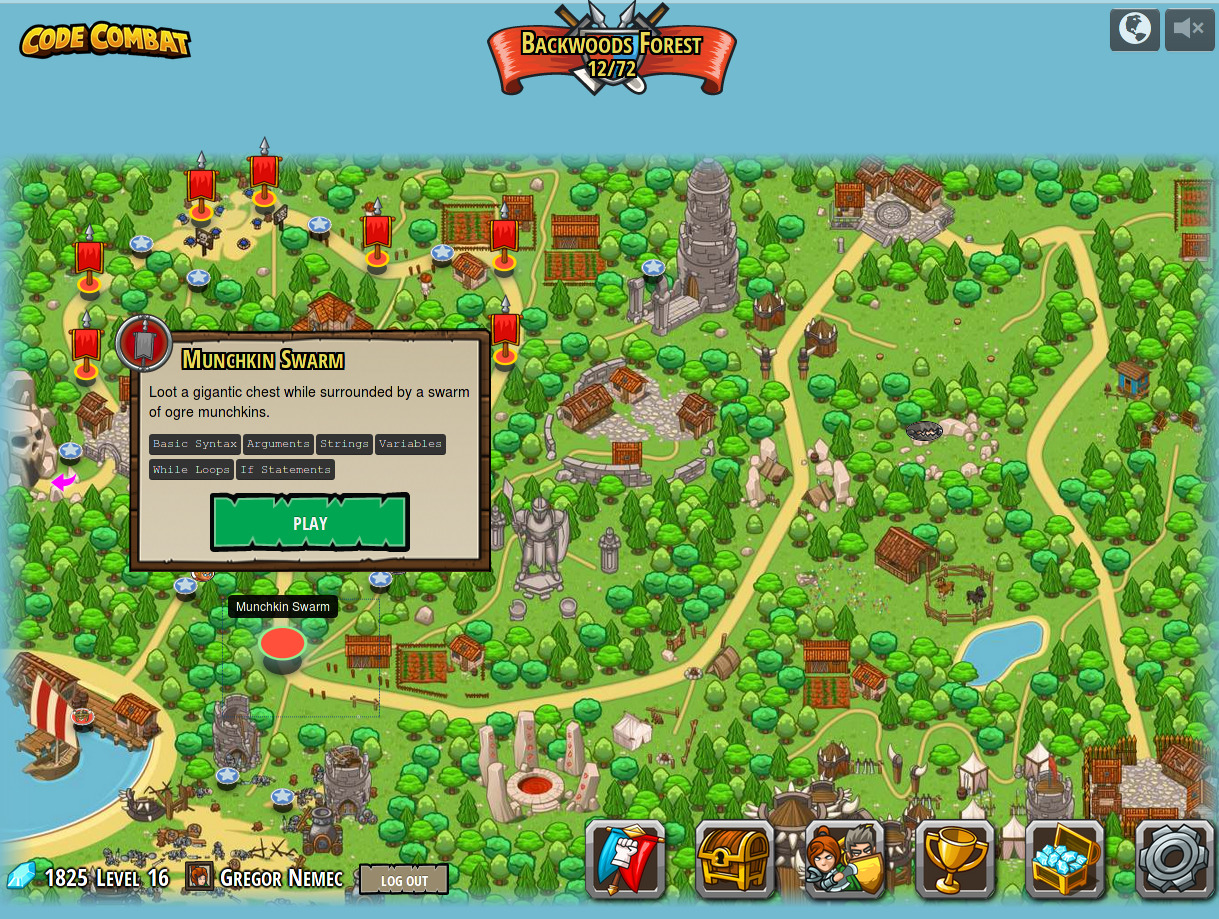
\includegraphics [width=0.65\linewidth, keepaspectratio =
   1] {./images/sc_web/cc_izbor-zem-BG-v01.jpg}
   \caption{Podroben zemljevid za izbiro nalog \cite{web:codecombat}.}
   \label{fig:web:cc:zemljevid:BG}
 \end{figure}

 Sledi opremljanje junaka (slika \ref{fig:web:cc:zemljevid:EQ}). Igra
 tu pomaga v tolikšni meri, da omeji nekatere predmete, ki niso
 uporabni za trenutno nalogo. Sledimo logiki igre in izbiramo
 vedno najboljšo opremo, ki je na voljo.
 
\begin{figure}[h!]
  \centering
    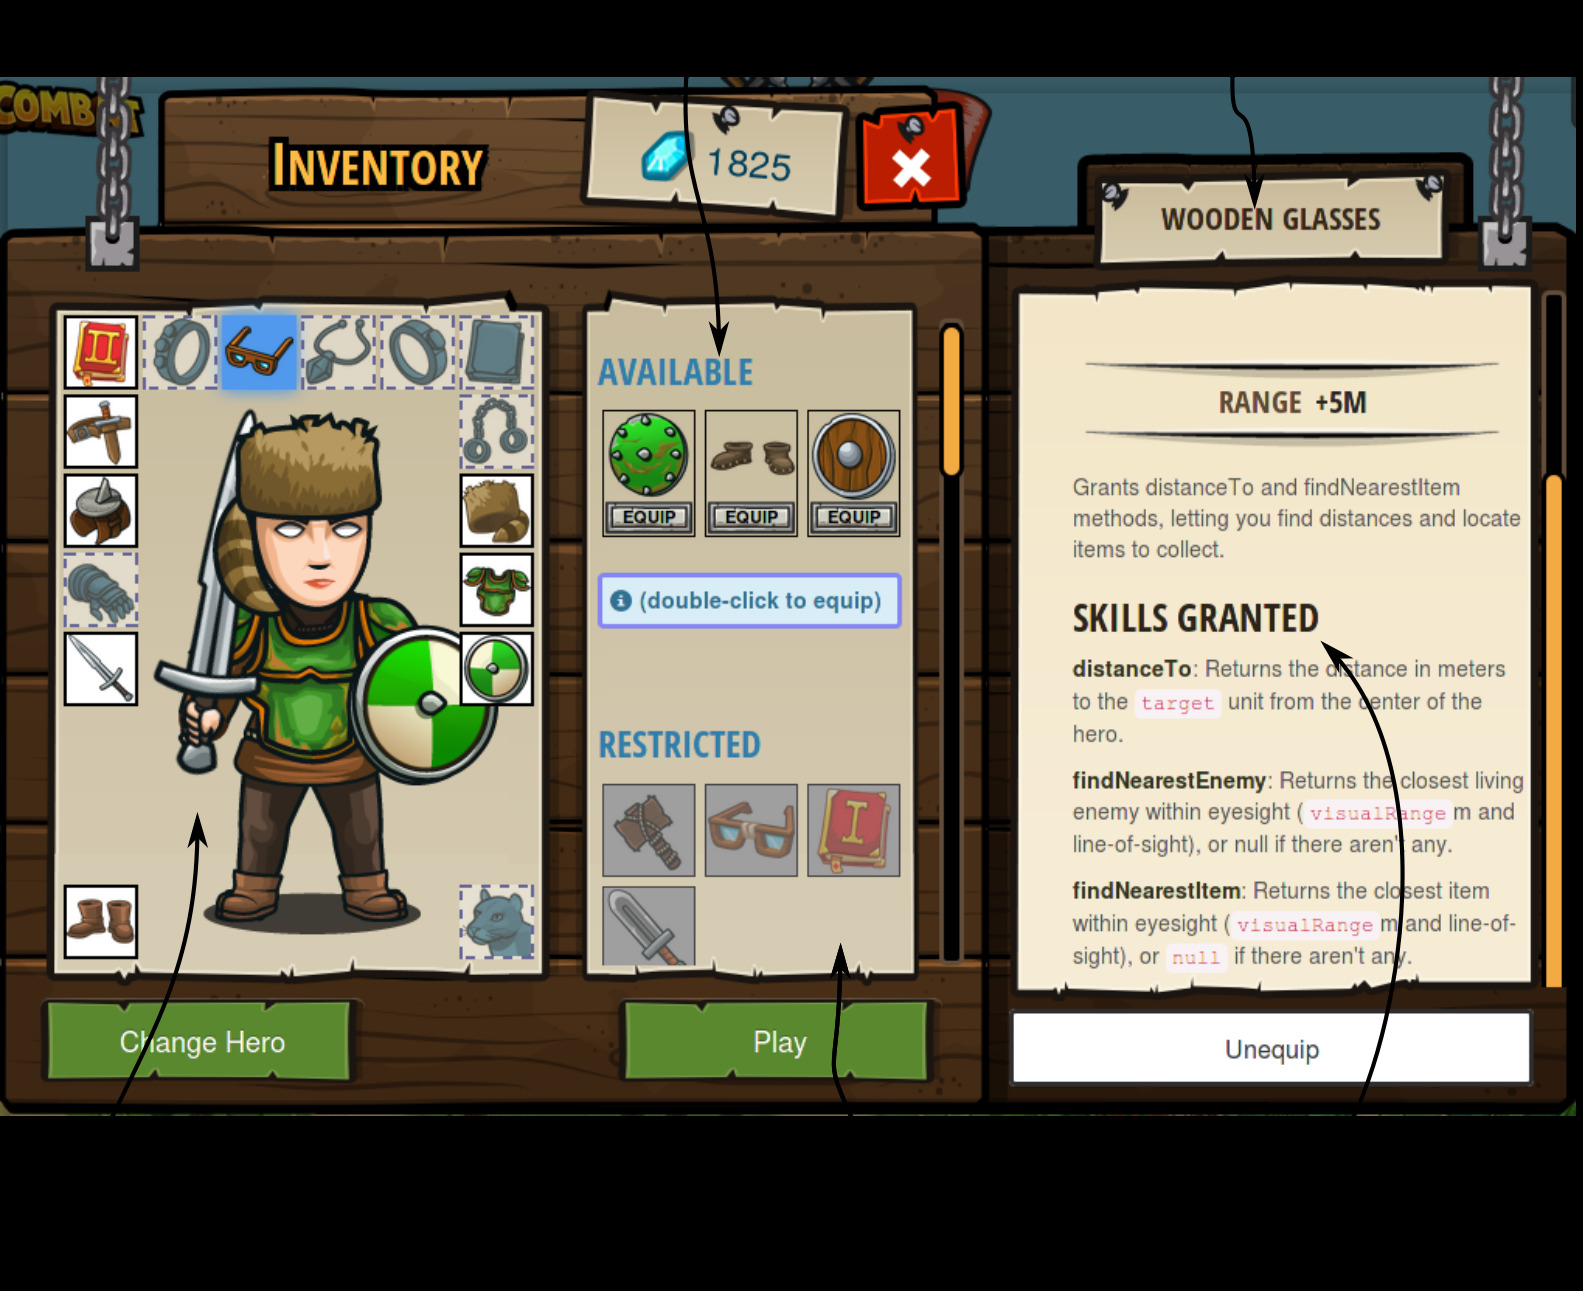
\includegraphics [width=0.55\linewidth, keepaspectratio =
   1] {./images/sc_web/cc_izbor-zem-EQ-v01.jpg}
   \caption{Oprema junaka in njen opis \cite{web:codecombat}.}
   \label{fig:web:cc:zemljevid:EQ}
 \end{figure}
 
 Ko kažemo ta primer igre, smo z napredkom rešenih nalog skoraj na
 polovici drugega zemljevida in so oprema in veščine, ki jih uporablja
 naš junak, že napredne, zato naredimo primerjavo med prejšnjo in
 nadgrajeno opremo. S primerjavo škornjev (slika \ref{fig:cc:eq:sb} in
 \ref{fig:cc:eq:lb}) lahko povzamemo, katere metode je junak
 pridobil. Če je pri \emph{preprostih škornjih} imel možnost gibanja
 le v smeri \textbf{levo, desno, gor in dol}, se lahko pri
 \emph{usnjenih škornjih} giblje po najkrajši poti na koordinate, ki
 jih podamo kot argument metode \texttt{hero.moveXY(x,z)}. S
 primerjavo \emph{knjige za programiranje} med različico \emph{I in II}
 (slika \ref{fig:cc:eq:p1} in \ref{fig:cc:eq:p2}), ki smo jo pridobili
pozneje, je razlika med veščinami očitna. Če smo pri \emph{knjigi za
   programiranje I} lahko uporabljali samo zanke
 \texttt{\textbf{loop:}} oz. \texttt{\textbf{while True}:}, pri
 \emph{knjigi za programirane II} lahko zraven uporabljamo še
 \texttt{\textbf{if/else stavek}}. Primerjali smo samo dva predmeta,
 junaku so na voljo številni predmeti z različnimi metodami za
 različne dele telesa, vse od \textbf{mečev, ščitov, kap, ur, pasa,
   obleke, očal} in tako dalje. Z napredovanjem veščin in naborom
 predmetov junak pridobiva na zmožnostih, prav tako se s tem postopno
 izboljšujejo veščine in se širi znanje uporabniku spletne igre.

 \begin{figure}[h!]
    \centering
    \begin{subfigure}[]{0.25\textwidth}
      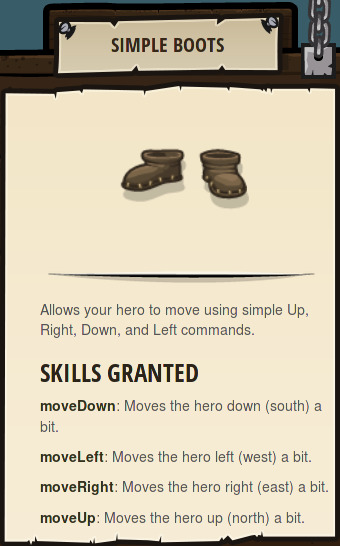
\includegraphics[width=\textwidth]{./images/sc_web/cc_EQ-SB-v01.jpg}
        \caption{Preprosti škornji (\emph{ang. Simple boots})}
        \label{fig:cc:eq:sb}
      \end{subfigure}
      \qquad
    \begin{subfigure}[]{0.25\textwidth}
        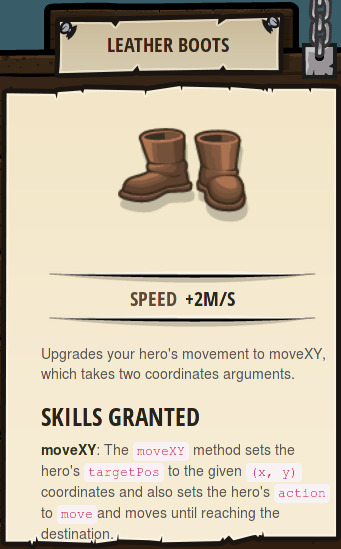
\includegraphics[width=\textwidth]{./images/sc_web/cc_EQ-LB-v01.jpg}
        \caption{Usnjeni škornji (\emph{ang. Lether boots})}
        \label{fig:cc:eq:lb}
    \end{subfigure}
    \\
    \begin{subfigure}[]{0.25\textwidth}
      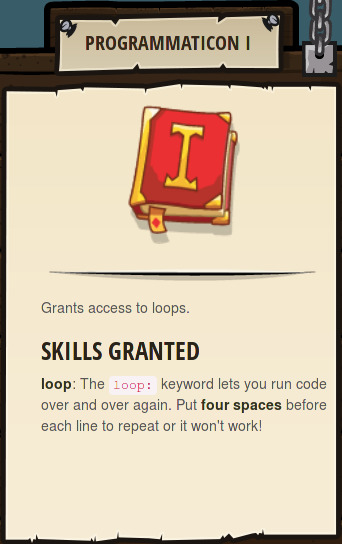
\includegraphics[width=\textwidth]{./images/sc_web/cc_EQ-P1-v01.jpg}
        \caption{Knjiga programiranja I}
        \label{fig:cc:eq:p1}
      \end{subfigure}
      \qquad
    \begin{subfigure}[]{0.25\textwidth}
        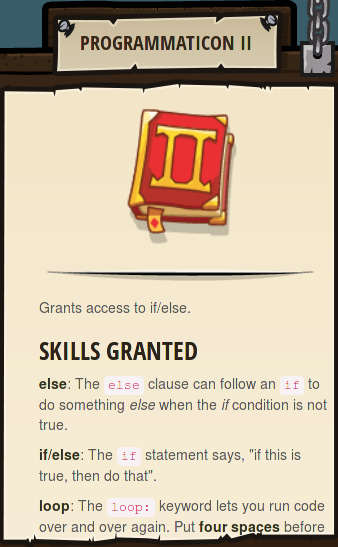
\includegraphics[width=\textwidth]{./images/sc_web/cc_EQ-P2-v01.jpg}
        \caption{Knjiga programiranja II}
        \label{fig:cc:eq:p2}
    \end{subfigure}
    \caption{Primerjava med prejšnjo različico opreme in njeno
      nadgradnjo, ki jo lahko zamenjamo junaku \cite{web:codecombat}.}
   \label{fig:web:cc:EQ:Primerjava}
\end{figure} 

%(slika \ref{fig:web:cc:ingame:cilji})
% \begin{figure}[h!]
%   \centering
%     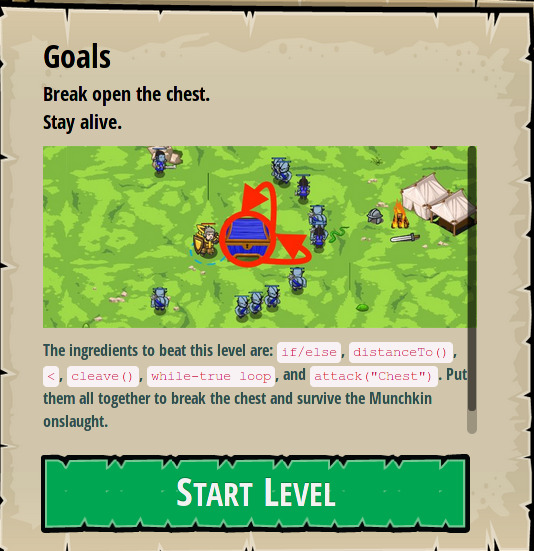
\includegraphics [width=0.35\linewidth, keepaspectratio =
%    1] {./images/sc_web/cc_ingame-goals-v01.jpg}
%    \caption{Prikaz ciljev v začetku igre \cite{web:codecombat}.}
%    \label{fig:web:cc:ingame:cilji}
%  \end{figure}

Po vsakem zagonu igre sledi najprej prikaz cilja, ki ga moramo
uresničiti. Postavitev igre (slika \ref{fig:web:cc:ingame:game}) je
taka, da nalogo rešujemo v \textbf{urejevalniku besedil}, ki je na
desni strani zaslona. Programska koda, ki jo izvajamo, se odvija v oknu
na levi strani. Urejevalnik besedil omogoča nekatere napredne
funkcije, kot je \textbf{barvanje kode, samodejno zamikanje vrstic,
  prikaz zamika vrstic, sprotno opozarjanje na napačno sintakso} ter
\textbf{predlogi za samodejno dokončanje} programske kode. Pri samem
pisanju programske kode lahko zapišemo na primer samo del metode, kot
je \texttt{find}, in se nam ob potrditvi samodejnega predloga izpiše
celotna programska koda \texttt{enemy = hero.findNearestEnemy()}.

\begin{figure}[h!]
  \centering
    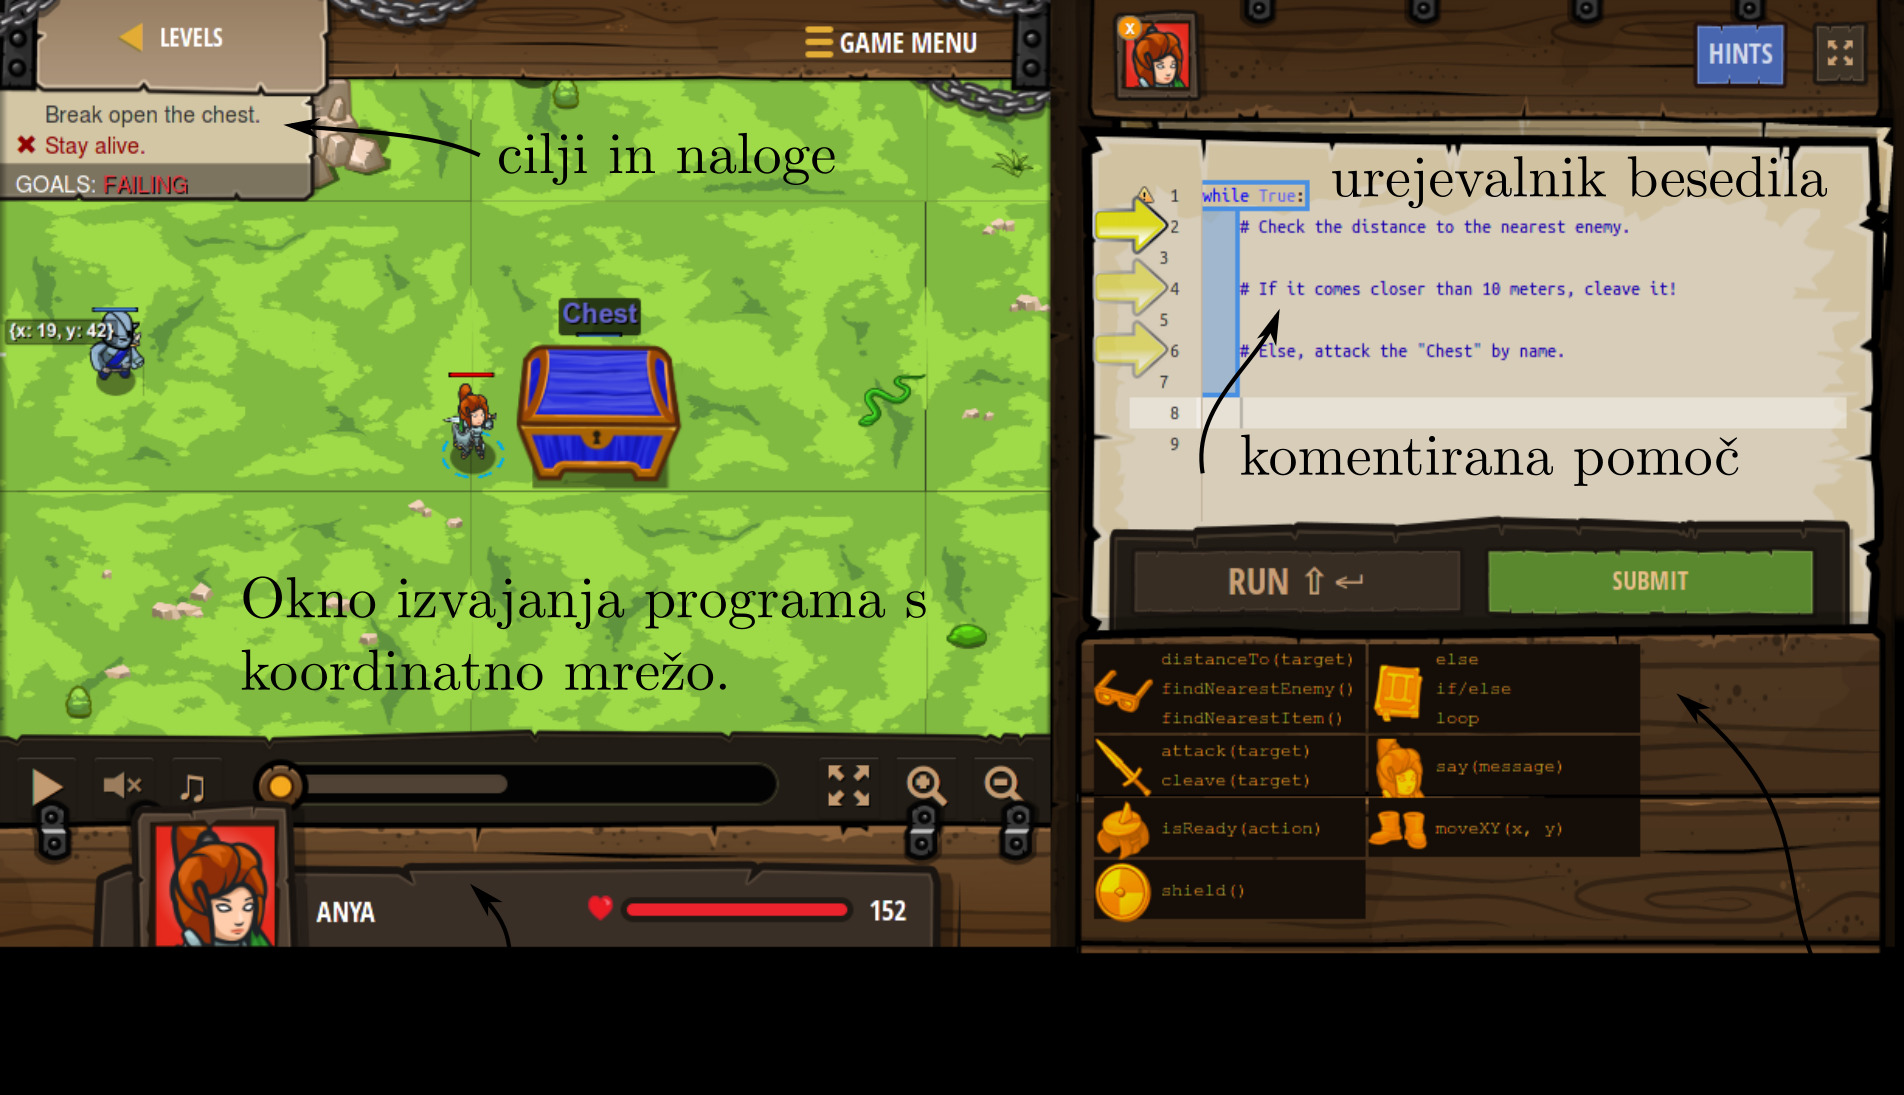
\includegraphics [width=0.55\linewidth, keepaspectratio =
   1] {./images/sc_web/cc_ingame-game-v01.jpg}
   \caption{Postavitev igre \cite{web:codecombat}.}
   \label{fig:web:cc:ingame:game}
 \end{figure}

 V trenutni nalogi je cilj tak, da moramo napadati sovražnike, ko je
 ta bližje skrinji kot \emph{10 m} in ga moramo napasti z metodo
 \texttt{cleve}, če  sovražnika ni v bližini, napadamo skrinjo. Ko
 smo zadovoljni s svojo rešitvijo, poženemo program in čakamo na končni
 izid (slika \ref{fig:web:cc:ingame:game2}). Če je iztek programa
 uspešen in smo rešili nalogo, jo \emph{posredujemo}.

\begin{figure}[h!]
  \centering
    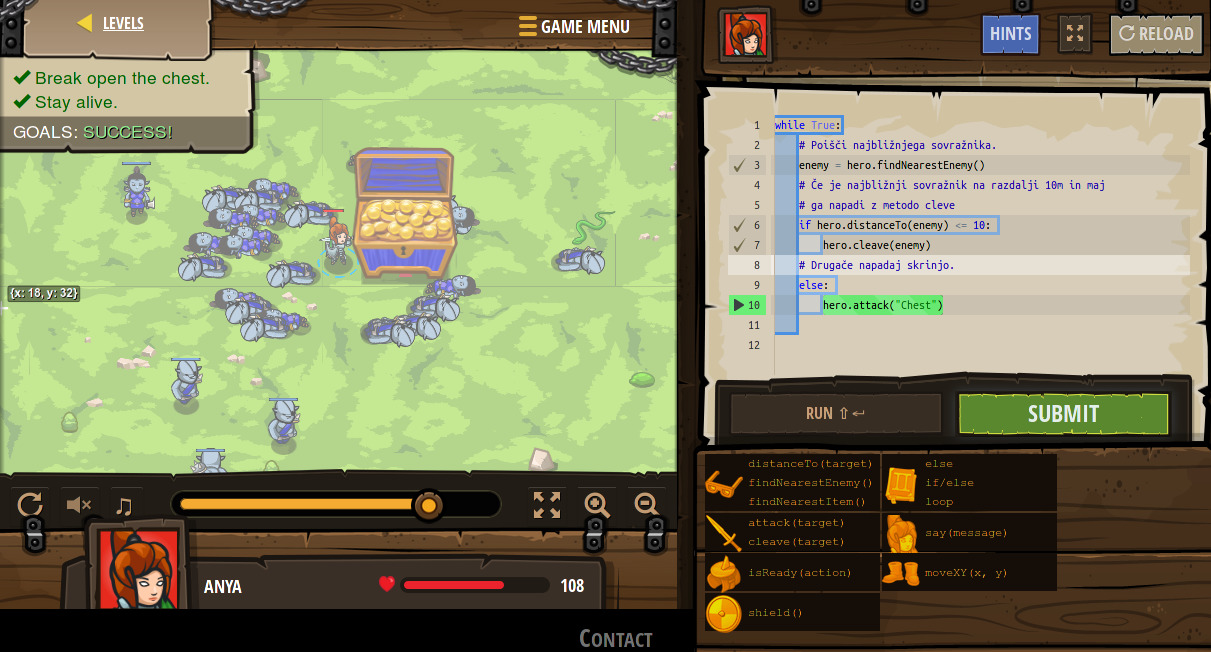
\includegraphics [width=0.55\linewidth, keepaspectratio =
   1] {./images/sc_web/cc_ingame-game-v02.jpg}
   \caption{Uspešno končan izid igre z napisano programsko
     kodo \cite{web:codecombat}.}
   \label{fig:web:cc:ingame:game2}
 \end{figure}
 
 Ob koncu igre poberemo še \textbf{dosežke}, to so \textbf{točke
   izkušenj}, \textbf{diamante} in \textbf{značke} (slika
 \ref{fig:web:cc:ingame:ach}) . 

\begin{figure}[h!]
  \centering
    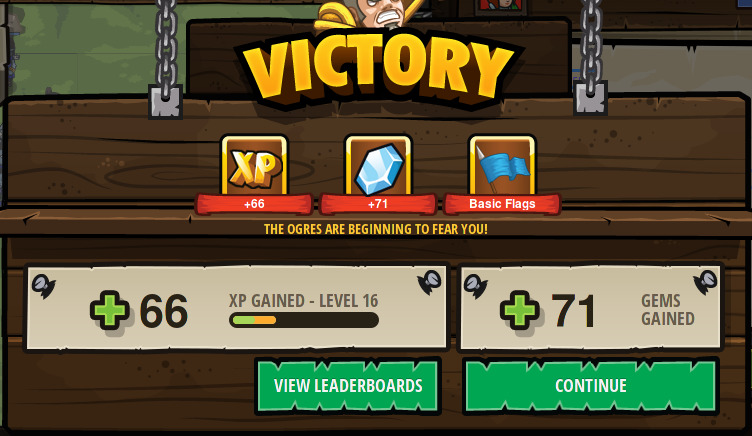
\includegraphics [width=0.35\linewidth, keepaspectratio =
   1] {./images/sc_web/cc_ingame-ach-v02.jpg}
   \caption{Končni rezultat in pregled nad dobljenimi dosežki ob koncu
     igre\cite{web:codecombat}.}
   \label{fig:web:cc:ingame:ach}
 \end{figure}

 Dostop do spletnega portala pa ni povsem brezplačen. Z
 \textbf{brezplačnim dostopom} lahko raziščemo 145 nalog v petih
 zemljevidih. Spletni portal ponuja \textbf{naročnino} 10 \$\ na mesec, s
 katero lahko pridobimo dodatne \textbf{naloge, junake, diamante} in
 tako dalje.
 
\subsubsection{Upravljanje razreda}
\label{sec:upravljanje_razreda_cc}

Spletni portal omogoča \textbf{upravljanje razredov}. Razrede upravlja
\textbf{učitelj}.  Portal ima prilagojeno učno snov za tri stopnje po
ameriškem \textbf{K-12} sistemu. Kot smo že primerjali šolske sisteme,
lahko povemo, da so stopnje po starosti v slovenski šoli prilagojene
na naslednje stopnje \textbf{osnovno šolo (2. triado in 3. triado) in
  srednjo šolo}. Upravljanje razredov (slika \ref{fig:web:cc:teach})
je podobno, kot smo to videli pri \textbf{Code academy} (poglavje
\ref{sec:uporaba_učitelji}). Učitelj ima nadzor nad dodajanjem učencev
in ima pregled o napredku učencev. Z njimi preko portala ne more
komunicirati.

\begin{figure}[ht!]
  \centering
    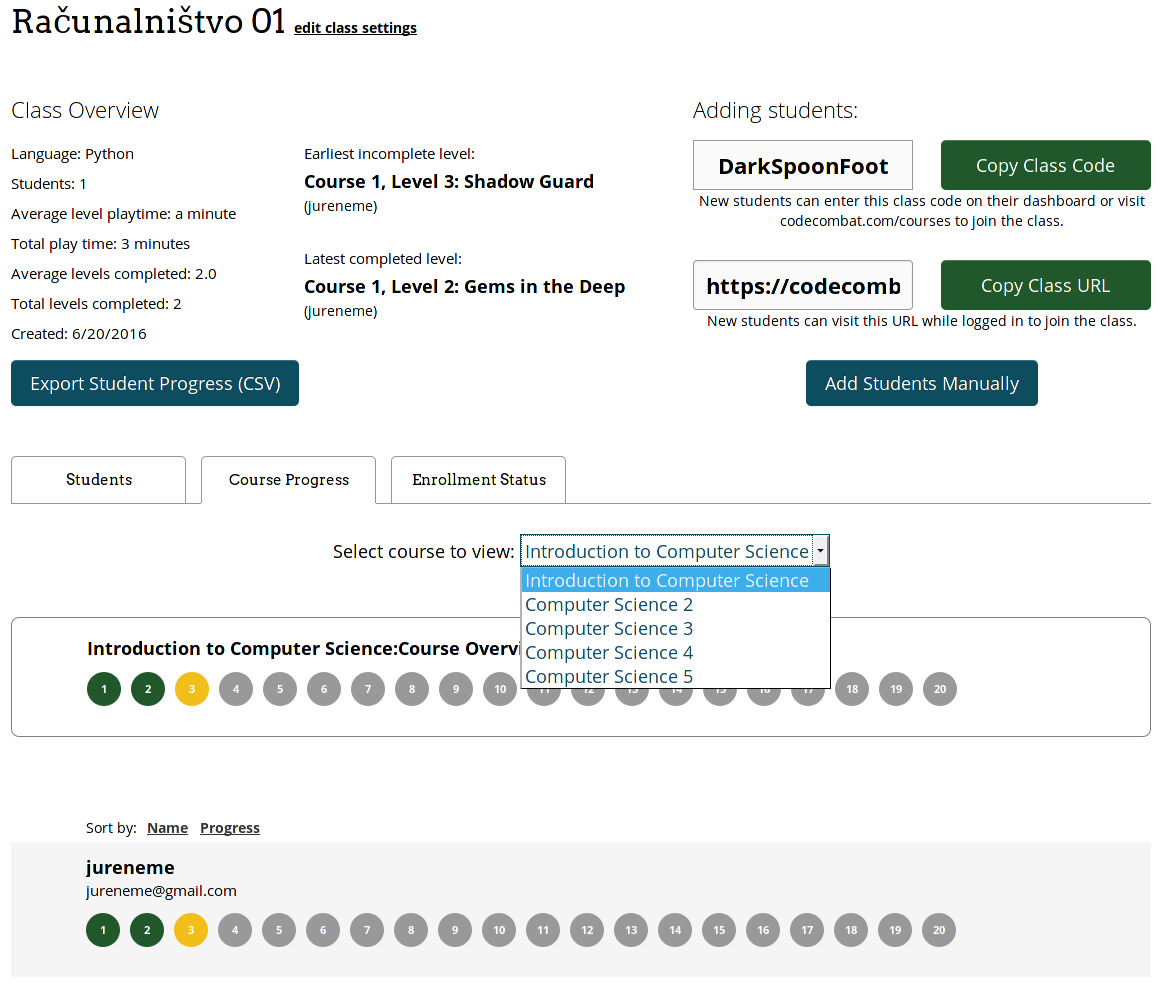
\includegraphics [width=0.75\linewidth, keepaspectratio =
   1] {./images/sc_web/cc_teach-clsv-v01.jpg}
   \caption{Učiteljev pogled na upravljanje razreda \cite{web:codecombat}.}
   \label{fig:web:cc:teach}
\end{figure}

Dostop \textbf{za šole ni brezplačen}. Učitelj lahko zahteva
demonstracijsko različico in v njo povabi neomejeno število učencev. V
tej demo različici je na voljo samo prvi tečaj \textbf{Uvod v
  računalniško znanost}, vsi ostali so zaklenjeni. Za uporabo
nadaljevalnih tečajev mora učitelj zaprositi za poizvedbo cene za nakup
licence za posameznega učenca.

Učenec rešuje naloge podobno, kot smo to lahko videli pri navadnem
računu, vendar ne more stopenj izbirati iz mape. Naloge oz. stopnje,
ki jih rešuje, so prilagojene tečaju, v katerega ga je vpisal
učitelj. Po opravljeni nalogi učenec takoj nadaljuje na naslednjo
stopnjo, kot je ta predvidena v tečaju. Učenec ima vpogled v naloge,
ki ga čakajo v tečaju. V seznamu lahko izbere tiste naloge, ki jih je
že opravil oz. tisto zadnjo, v kateri je ostal. Za nadaljevanje mora
učenec rešiti prejšnjo nalogo. Če v navadnem računu lahko menjujemo
različne dele oblačil in opreme, je to v načinu učenčevega načina
onemogočeno. Učenčev lik ima na voljo stvari, ki jih potrebuje pri
rešitvi naloge. S to omejitvijo je olajšano delo učitelja, saj se tako
lahko razred osredotoči le na reševanje naloge.

 %(slika \ref{fig:web:cc:stud})
% \begin{figure}[h!]
%   \centering
%     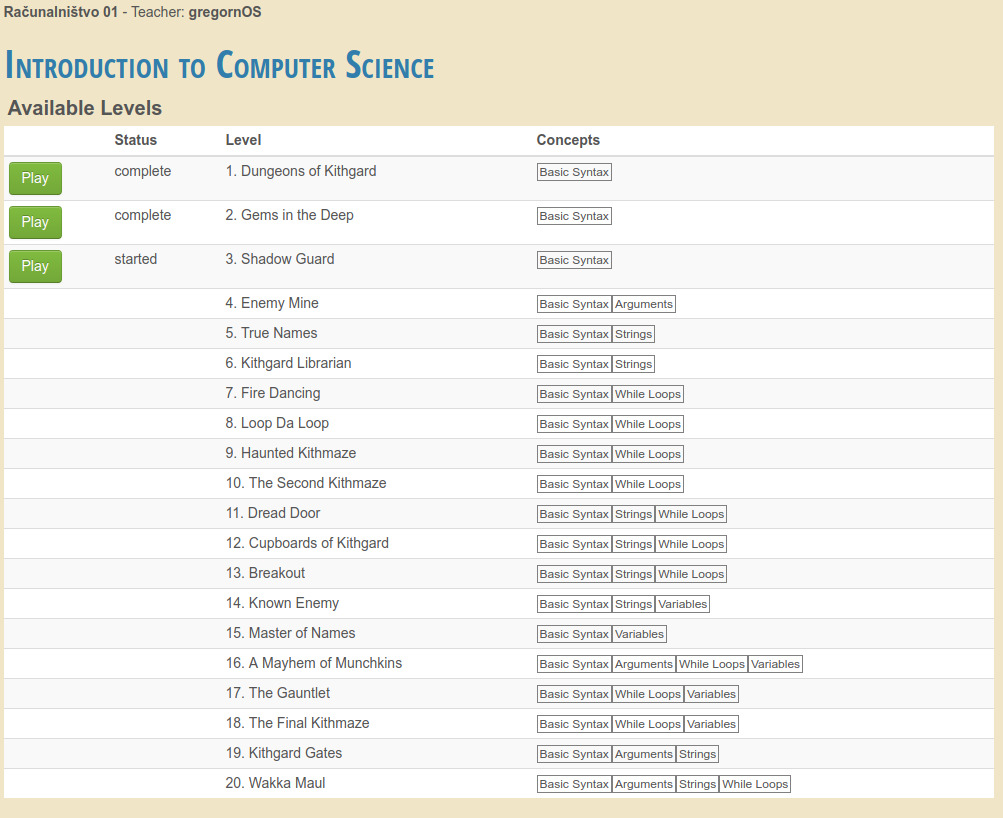
\includegraphics [width=0.65\linewidth, keepaspectratio =
%    1] {./images/sc_web/cc_stud-al-v01.jpg}
%    \caption{Učencev pogled na seznam nalog v tečaju \cite{web:codecombat}.}
%    \label{fig:web:cc:stud}
% \end{figure}

 Spletni portal ima prevode v več večjih svetovnih jezikov, žal
 trenutno slovenščina ni med njimi. V padajočem meniju, kjer učenci
 lahko spreminjajo jezike, se najde tudi slovenščina, vendar se ob
 njenem izboru prikaže pojavno okno s pozivom za prevod v izbran
 jezik. Uporabniku se ponudi spremenjen račun, ki omogoča prevajanje v
 druge jezike. Torej obstaja upanje, da se bo mogoče nekoč nekdo
 lotil tega projekta in začel prevajati spletni portal in naloge v
 slovenski jezik. 

\subsubsection{Povzetek}
\label{sec:povzetek:codecombat}

Spletni portal oz. spletna igra ima vsekakor veliki motivacijski
faktor. Naloge so narejene sistematično in postopno. Čeprav se v
naših osnovnih šolah ne priporoča učenje programskih jezikov, kjer
pišemo programsko kodo, razen morda \textbf{Logo}, naj bi se
uporabljali vizualni programski jeziki, kot je \textbf{Scratch}. Za ta
spletni portal verjamemo, da bi ga lahko uporabili pri osnovnošolcih,
ki bi lahko poučevali \textbf{Python}. Težava je edino
\textbf{slovenščina}, saj na strani še ni prevoda nalog, in
\textbf{plačljivost} za uporabo razredov. To učitelj sicer lahko
zaobide z uporabo \textbf{navadnih računov} in uporabo brezplačnih
vsebin, vendar mu to uteži delo, ali pa zaprosi za demonstracijsko
različico in v ta namen izkoristi vsebine, ki so na voljo brezplačno. 

\begin{osebnabox}[label={osebna:codecombat}]{Codecombat |
    \url{https://codecombat.com/}}
    \begin{tabular}{
  p{0.30\linewidth-2\tabcolsep} |
  p{0.70\linewidth-2\tabcolsep}  }
  \textbf{Vrsta vsebine} & Spletna igra za programiranje. Kombinacija
                           igre RPG + pisanje programske kode. \\
      \hline
  \textbf{Jezik spletne strani} & Angleščina: da, slovenščina: ne,
                                  drugi: da. \\
      \hline
  \textbf{Ponujena znanja} & Znanja programskih jezikov in  algoritmov. \\
      \hline
 \textbf{Programski jeziki} & Python, JavaScript, CoffeScript, LUA. \\  
      \hline
  \textbf{Težavnostna stopnja} & Osnovna šola (2/3 in 3/3) in srednja
                                 šola. \\ 
      \hline
   \textbf{Upoštevanje načel} & Problemski pristop: da,
                                sistematičnost: da, postopnost: da. \\
      \hline
  \textbf{Dosežki/Gamification} & Da (značke, izkušnje, diamanti). \\
      \hline
  \textbf{Dodajanje lastnih vsebin} & Ne. \\
      \hline
  \textbf{Upravljanje razreda} & Da (za osnovni tečaj brezplačno, za
                                 ostale tečaje plačljiva licenca). \\ 
      \hline
  \textbf{Dostop vsebin} & Polplačljiv: brezplačnih je 145 nalog,
                           plačljive so dodatne naloge - 95, dodatni
                           diamanti … za (9,99\$/mesec).   \\  

\end{tabular}
\end{osebnabox}

\subsection{Codingame}
\label{sec:codingame}

Spletni portal \emph{\href{https://www.codingame.com}{Codingame}}
\cite{web:codingame} je spletna igra, katere bistvo je, da uporabnik
rešuje probleme, ki so zahtevni in so predstavljeni kot izzivi v
obliki igre. Uporabnik s podajanjem rešitev izboljšuje veščine
programiranja in znanje algoritmov.

Za vsakega uporabnika se igranje oz. reševanje problemov začne pri
\textbf{sestavljankah} (\emph{ang. puzzles}) (slika
\ref{fig:web:ca:puzz}). V enoigralskem načinu so igre razdeljene na
več težavnosti, vse od \textbf{lahkih} do \textbf{zelo težkih}. Na tej
strani lahko izbiramo med sestavljankami, kjer imamo nalogo, da
programsko kodo čim bolj \textbf{optimiramo}
(\emph{ang. optimisation}), torej poiščemo rešitev, ki potrebuje
najmanjšo časovno in prostorsko zahtevnost. Druga vrsta iger je taka,
da s čim manj kode, torej znanjem trikov programskega jezika, rešimo
problem na strani \emph{ang. Code golf}. Imamo še možnost, da
rešujemo naloge, ki jih je pripravila skupnost, na strani
\emph{ang. Community puzzles}. Na tej strani se lahko posredujejo
lastne naloge, ki pa morajo biti odobrene s strani razvijalcev spletne
strani, preden se objavijo.  

\begin{figure}[h!]
  \centering
    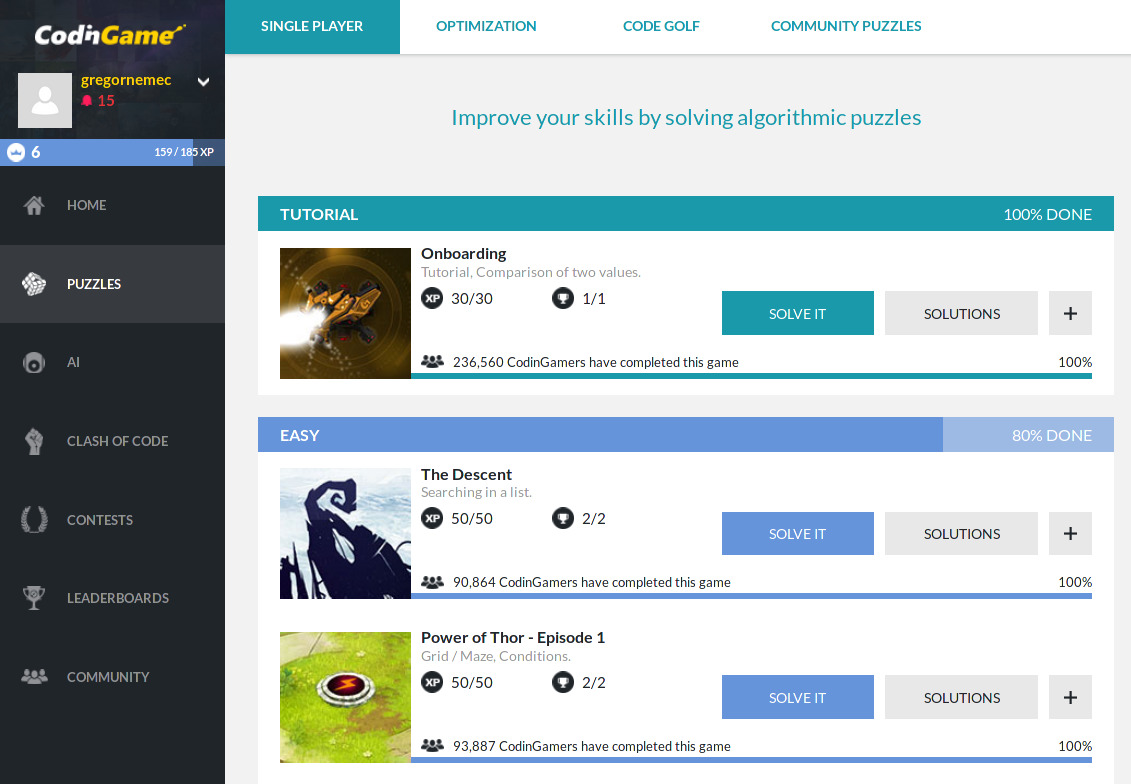
\includegraphics [width=0.75\linewidth, keepaspectratio =
   1] {./images/sc_web/codingame_puzz-v01.jpg}
   \caption{Podstran \emph{\href{https://www.codingame.com}{Codingame}}
\cite{web:codingame} - sestavljanke.}
   \label{fig:web:ca:puzz}
 \end{figure}

 Poglejmo, kako rešujemo problem. V ta namen smo izbrali sestavljanko
 \textbf{Most - Episoda I} (\emph{ang. The bridge - Episode I}) (slika
 \ref{fig:web:ca:solve}). Za reševanje naloge lahko izbiramo med
 številnimi programskimi jeziki, kot so \textbf{C\#, C++, Java,
   JavaScript, Python3, Bash, C, Clojure, Dart, F\#}. V našem primeru
 bomo uporabili programski jezik \textbf{Python3}.
 
 Primer izbrane naloge pravi, da moramo napisati program, ki upravlja
 hitrost motorja, ki se vozi po mostu in mora preskočiti prepad
 ter se na koncu pravočasno ustaviti. Celoten program teče v neskončni
 \texttt{while True} zanki. Na vsakem koraku moramo izpisati, kaj je
 naslednja akcija motorja ali naj \texttt{POSPEŠI, ČAKA, ZAVIRA}
 ali \texttt{SKOČI}. Na vsakem koraku se hitrost poveča oz. zmanjša za
 1. \texttt{Hitrost} se na vsakem koraku odraža za razdaljo, ki je
 enaka hitrosti. Vhodni podatki programa so naslednji, \texttt{cesta},
 ki je razdalja pred \texttt{prepadom}, naslednji podatek je velikost
 \texttt{prepada} in razdalja \texttt{zaviralne poti}.

 Na levi strani zgoraj \textbf{opazujemo potek rešitve}. Levo v
 sredini so napisana \textbf{navodila}, ki natančno opišejo problem,
 \emph{vhodne podatke, omejitve } in pričakovan \emph{izpis programa}
 na vsakem koraku. Levo spodaj je \emph{ukazna vrstica}, na kateri
 spremljamo izpis programa in ki nam je v pomoč pri razhroščevanju.

 Na desni strani je \textbf{urejevalnik besedil}, v katerega pišemo
 rešitev oz. program. Urejevalnik zna barvati programsko kodo,
 samodejno upošteva zamik programske kode in podaja samodejne predloge
 za metode, ki so vgrajene, ko napišemo ``.''. V nastavitvah
 urejevalnika lahko izbiramo način, ki prilagodi vedenje in ga lahko
 nastavimo na \emph{klasičen, emacs} in \emph{vim} način. Izbiramo
 lahko med temno in svetlo barvno shemo. Nastavimo lahko samodejno
 zaključevanje oklepajev.

 Spodaj desno poganjamo program s \textbf{testnimi primeri}, ki
 rešitev testirajo v skrajnih mejah. Testi, ki so podani kot
 vhodni podatki, so narejeni tako, da onemogočajo, da bi napisali
 program, ki bi imel statično vgrajene rešitve. Ko rešitev prestane
 vse teste, jo lahko posredujemo. 

\begin{figure}[h!]
  \centering
    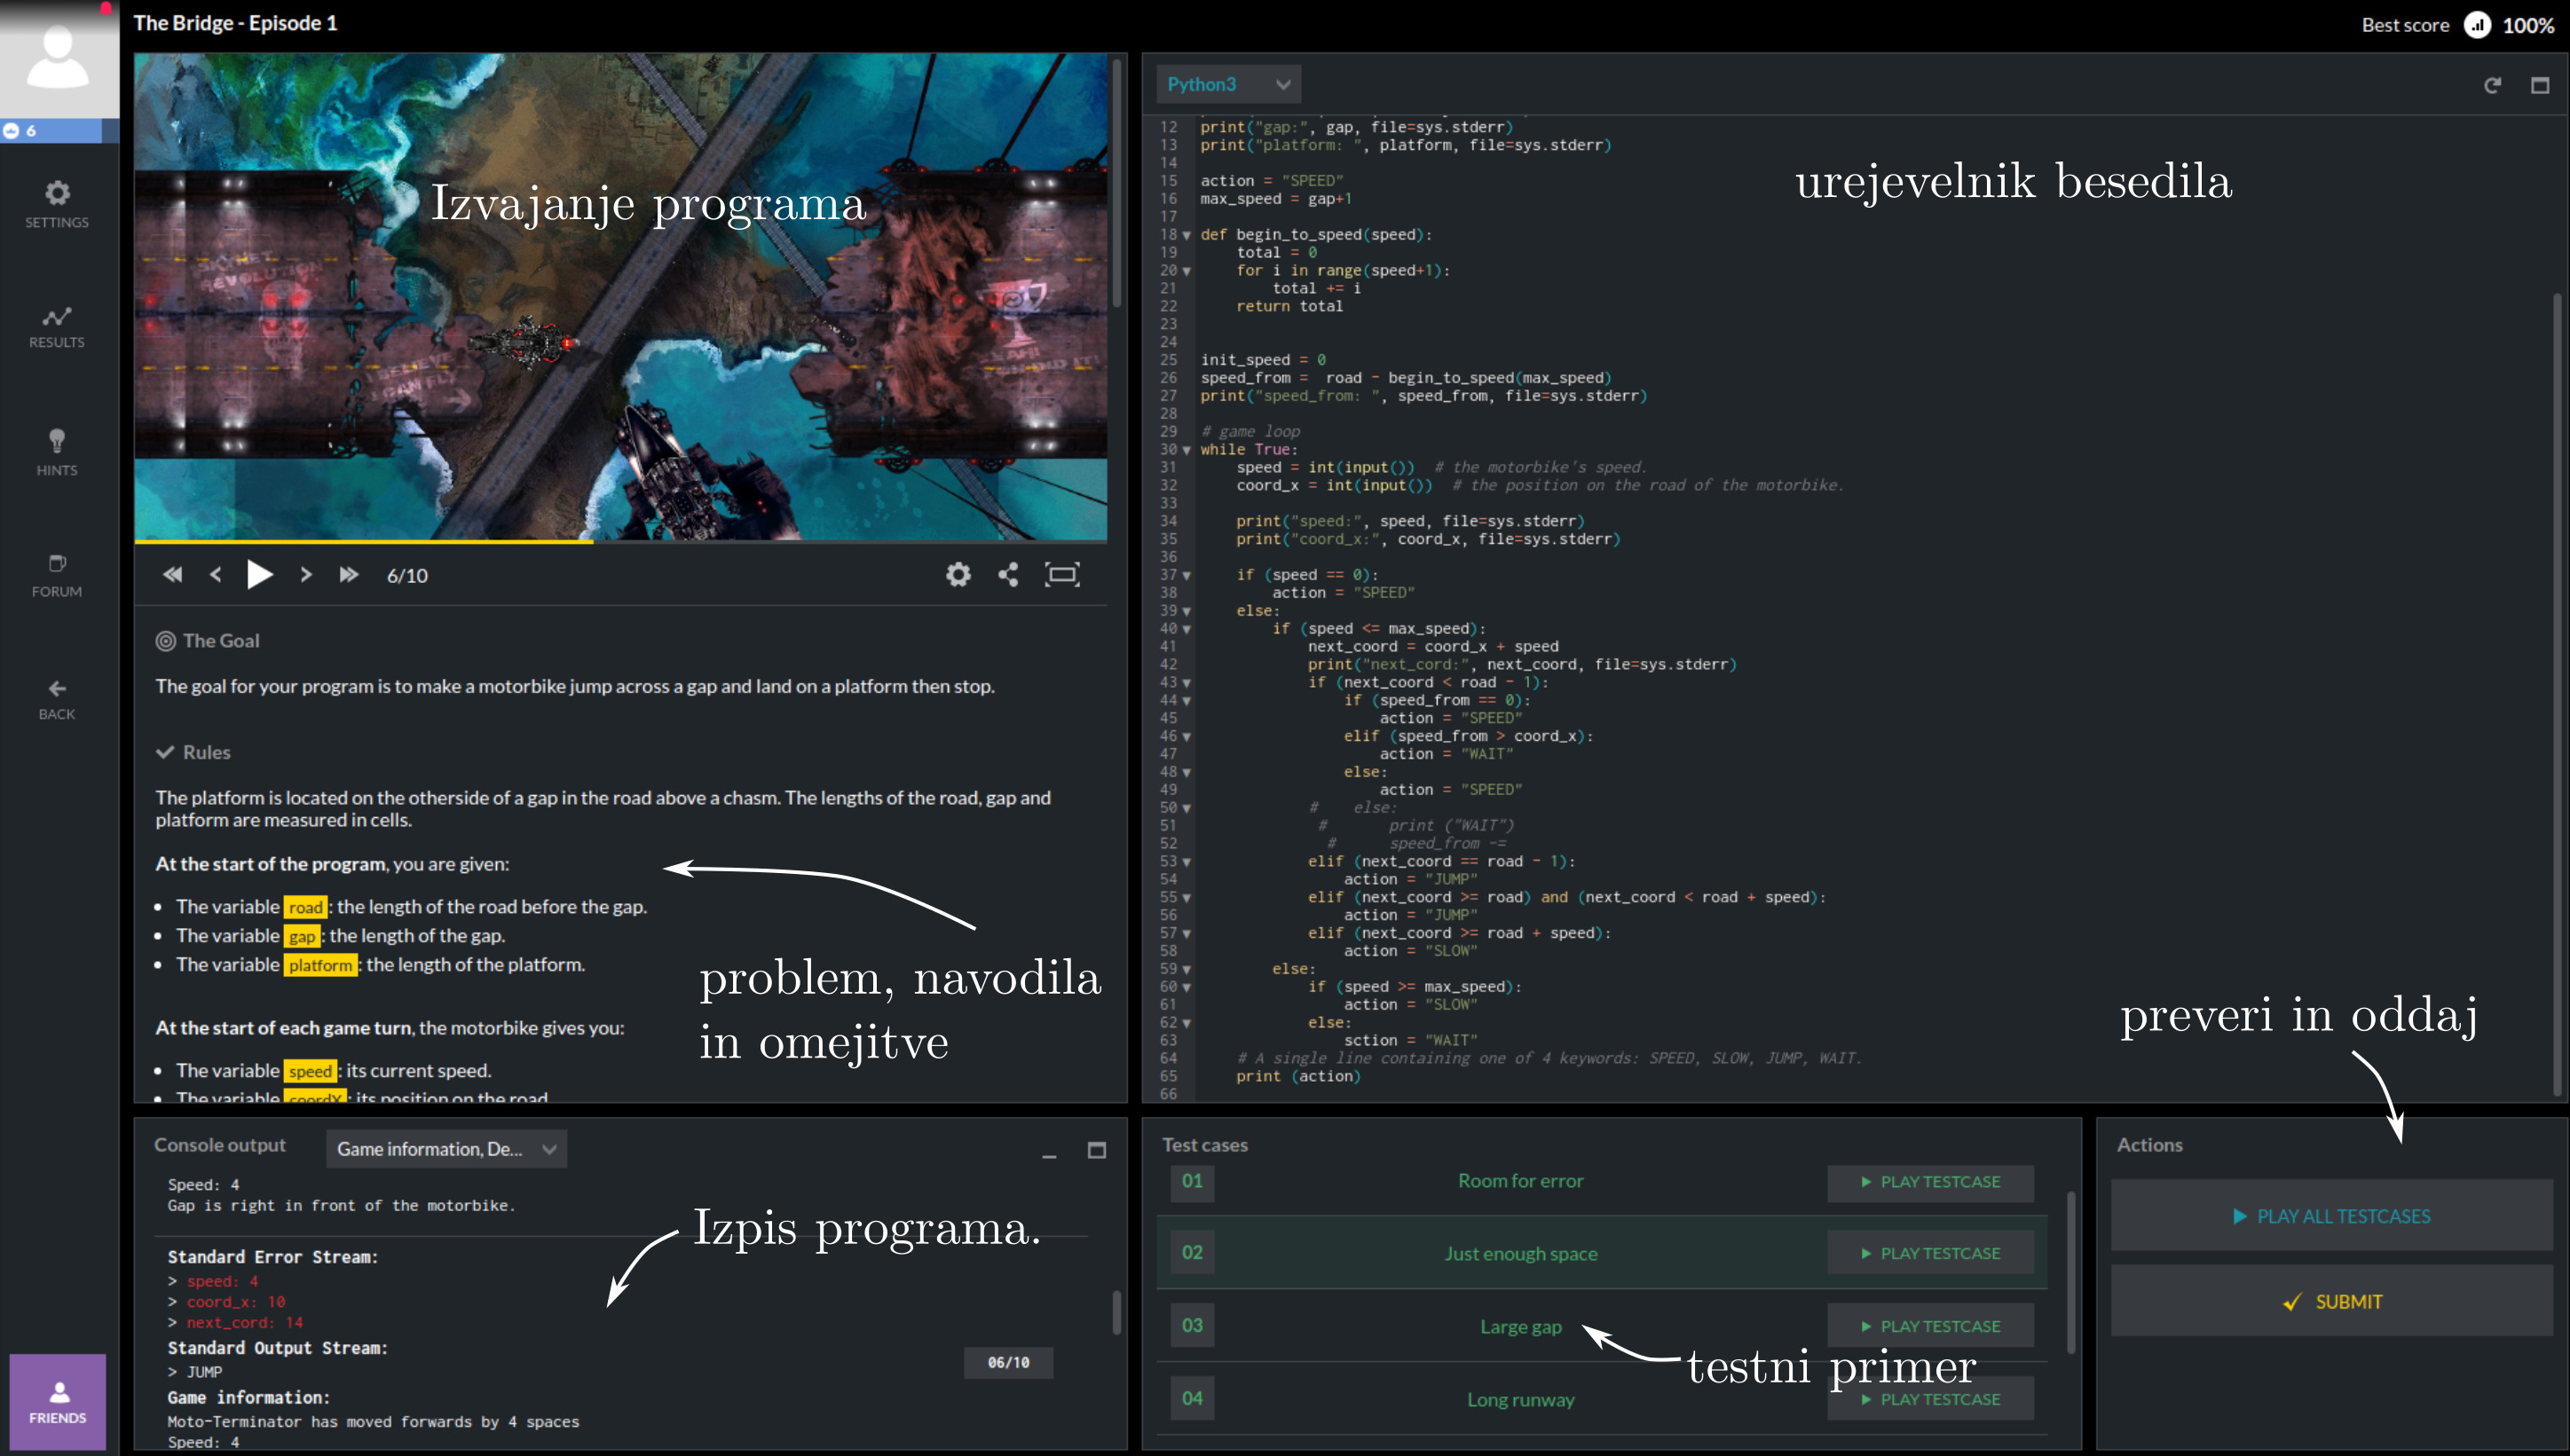
\includegraphics [width=1\linewidth, keepaspectratio =
   1] {./images/sc_web/codingame_solving-v01.jpg}
   \caption{Reševanje sestavljanke \emph{The Bridge}
     \cite{web:codingame}}
   \label{fig:web:ca:solve}
 \end{figure}

 Pri reševanju problemov se uči tudi življenjski krog razvijanja
 programske opreme in strategije reševanja problemov, kot smo jih
 opisali v poglavju \ref{sec:strategije_reševanja_problemov}, saj
 \textbf{problem najprej analiziramo, izberemo pristop, ga
   razgradimo, razvijemo algoritem in testiramo njegovo
   pravilnost}. Ta postopek lahko ponavljamo v krajših korakih, dokler
 ne pridemo do prave rešitve in ponovimo faze razvoja in testiranja
 algoritma večkrat. Ko algoritem reši problem, se lahko ukvarjamo z
 njegovo \textbf{učinkovitostjo}, ki jo pridobimo z upoštevanjem
 lastnosti implementacije algoritmov, torej časovne in prostorske
 zahtevnosti ter značilnosti programskega jezika in njegovih
 zmožnosti. Na tak posreden način nas spletni portal uči programski
 jezik, saj rešitev od nas zahteva optimalno rešitev, ki jo lahko
 dosežemo z dobrim poznavanjem programskega jezika in njegovih
 knjižnic.

 Med reševanjem si lahko pomagamo z \emph{namigi} in \emph{pseudo
   kodo}. Ko rešitev oddamo, sledi izračun točk in nagrad v obliki
 \textbf{točk izkušenj} in \textbf{značk}. Uporabnik lahko brska
 med rešitvami drugih uporabnikov in tako nabira dodatno znanje.

 Na spletni strani obstajajo še drugi načini igranja. Lahko se
 včlanimo v različne igre, kjer programiramo \textbf{bota}, ki
 tekmuje z \textbf{umetno inteligenco} na podstrani
 \emph{ang. AI}. \textbf{Spopad kode} ali \emph{ang. Clash of code} je
 način, v katerem do 8 igralcev tekmuje eden proti drugemu v bojih po
 5 ali 10 minut. Vsak zase rešuje problem, na koncu zmaga najbolj
 točkovana rešitev. Spletni portal prireja tudi uradna
 \textbf{tekmovanja}, na katerih se brezplačno registriramo. Izbiramo
 lahko med dvema sistemoma nagrajevanja, ali so nagrade v fizični
 obliki, kot je npr. 3D-tiskalnik, majice in podobno, ali se odločimo
 za način, kjer se potegujemo za razgovor na določenem delovnem mestu,
 ki je takrat razpisano. To je dober koncept prepoznavanja talentov in
 iskanja službe.
 
\subsubsection{Povzetek}
\label{sec:povzetek_codingame}

Spletni portal je namenjen predvsem treniranju veščin programiranja
in učenju algoritmov. Uporabnik mora poznati več kot le osnove
programiranja, zato je spletni portal namenjen predvsem za srednje
šole, višje in univerzitetne programe študija. Spletna igra ni
primerna za pouk, je pa lahko zelo dobro dopolnilo za dodatno vajo ter
izpopolnjevanje lastnih izkušenj programiranja. Priporočamo ga lahko
vsakemu, ki ga zanima programiranje. Sistem nalog in reševanja je
dobro zasnovan. Problemsko je zasnovano tudi ozadje vsake
naloge. Naloge si po težavnosti sledijo postopoma, sistematično so
naloge razmetane po vseh težavnostih stopnjah, zato ne moremo potrditi
načela sistematičnosti. 

\begin{osebnabox}[label={osebna:codingame}]{Codingame |
    \url{https://www.codingame.com}}
    \begin{tabular}{
  p{0.30\linewidth-2\tabcolsep} |
  p{0.70\linewidth-2\tabcolsep}  }
  \textbf{Vrsta vsebine} & Vadnica: spletna aplikacija za
                           programiranje + reševanje problemov +
                           testiranje). \\
      \hline
  \textbf{Jezik spletne strani} & Angleščina: da, slovenščina: ne,
                                  drugi: da. \\
      \hline
  \textbf{Ponujena znanja} & Znanje algoritmov in veščine programiranja. \\
      \hline
 \textbf{Programski jeziki} & C\#, C++; Java, JavaScript, Python3,
                              Bash, C, Clojure, Dart, F\# .\\  
      \hline
  \textbf{Težavnostna stopnja} & Srednja šola, visoki, višji in
                                 univerzitetni. \\ 
      \hline
   \textbf{Upoštevanje načel} & Problemski pristop: da,
                                sistematičnost: ne, postopnost: da. \\
      \hline
  \textbf{Dosežki/Gamification} & Da, značke, izkušnje, rangiranje. \\
      \hline
  \textbf{Dodajanje lastnih vsebin} & Da. Dodajanje lastnih
                                      nalog/problemov, ki jih rešuje
                                      skupnost. \\
      \hline
  \textbf{Upravljanje razreda} & Ne. \\ 
      \hline
  \textbf{Dostop vsebin} & Brezplačno   \\  

\end{tabular}
\end{osebnabox}


%%% Local Variables:
%%% mode: latex
%%% TeX-master: "../diploma"
%%% End:
